\documentclass[a4paper,reqno]{article}

\usepackage[T1,T2A]{fontenc}
\usepackage[utf8]{inputenc}
\usepackage[english,russian]{babel}
\usepackage{amsmath,amsthm,amssymb}
\usepackage{mathtext}
\usepackage{amsthm}
\usepackage{graphicx}
\usepackage{cmap}
\usepackage{bbm}
\usepackage{tikz}

% Types

\newtheorem{theorem}{Теорема}
\newtheorem{lemma}{Лемма}
\newtheorem{prop}{Утверждение}
\newtheorem{col}{Следствие}

\theoremstyle{definition}
\newtheorem{definition}{Определение}

\theoremstyle{definition}
\newtheorem{example}{Пример}

\theoremstyle{definition}
\newtheorem{nb}{Замечание}

\newcommand{\hm}[1]{#1\nobreak\discretionary{}{\hbox{\ensuremath{#1}}}{}}
\newcommand{\nn}{\nonumber}
\DeclareMathOperator{\sgn}{sign}
\DeclareMathOperator*{\E}{\mathbb{E}}
\DeclareMathOperator*{\var}{var}   
\DeclareMathOperator*{\Var}{Var}     
\DeclareMathOperator*{\cov}{cov}

\newcommand{\1}{\mathbbm{1}} %Indicator: \1 (X<5)
\newcommand{\Co}{\mathbb{C}}
\newcommand{\R}{\mathbb{R}}
\newcommand{\N}{\mathbb{N}}
\renewcommand{\P}{P}
\newcommand{\eps}{\varepsilon}
\renewcommand{\phi}{\varphi}

\numberwithin{equation}{section}
\numberwithin{theorem}{section}
\numberwithin{lemma}{section}
\numberwithin{prop}{section}
\numberwithin{col}{section}
\numberwithin{definition}{section}
\numberwithin{example}{section}
\numberwithin{nb}{section}

\usepackage{hyperref}
\hypersetup{
	colorlinks=true,
	linkcolor=blue,
	filecolor=magenta,      
	urlcolor=cyan,
}

\date{Весенний семестр 2021}
\title{Курс <<Теория вероятностей>>}
\author{Александр Вадимович Булинский}

\begin{document}
	\begin{titlepage}
		\maketitle
		
		\begin{abstract}
			Конспект подготовлен дилетантами, содержит кучу опечаток (2 и 8 лекции лучше не видеть, но главную идею понять несложно) и не является материалом, по которому стоит готовиться на 5. 
			Пишущий эти строки человек рекомендует пользоваться книгой Альберта Николаевича Ширяева <<Вероятность I>>, а еще лучше посещать лекции Александра Вадимовича. Но если вам теория вероятностей нужна только для того, чтобы ее сдать, то можно готовиться по этим конспектам.
			В целях более логичного изложения на бумаге редактор отступает от разбиения по лекциям и некоторые теоремы или утверждения относит туда, где они должны быть.
			Разбиение по подсекциям примерно соответствует программе экзамена 2021 года.

			\

			Литература, рекомендованная А. В. Булинским:
			\begin{itemize}
				\item \href{http://library.lol/main/fc60eb084dd543b1c3c699f545d7b697}{А. Н. Ширяев -- Вероятность-1}
				\item \href{http://library.lol/main/6BBA7CB717CA9C2CA0E6B8C1ECBFCB6C}{В. Феллер -- Введение в теорию вероятностей и ее приложения}
				\item \href{http://library.lol/main/78F07FA47D680D06414A642F6EDAE3F5}{А. А. Боровков -- Теория вероятностей}
				\item \href{http://library.lol/main/F3C74A3B4B64FB4DA8A2C8FD603DC09A}{Б. В. Гнеденко -- Курс теории вероятностей}
				\item \href{http://library.lol/main/174920B0DF85CC28BD6F4EE1DBFA0C0E}{Л. Б. Коралов, Я. Г. Синяй -- Теория вероятностей и случайные процессы}
				\item \href{http://library.lol/main/355BB740EEC2E4D0E359FC6CA5B61B4A}{J. Jacod, P. Protter -- Probability Essentials}
				\item \href{http://library.lol/main/BFBFB1676E70C977FC16BEDAB5E12234}{R. Durett -- Probability: Theory and Examples}
			\end{itemize}
			Все ссылки на июль 2021 года рабочие.
		\end{abstract}
	\end{titlepage}
	
	\tableofcontents
	\newpage
	\section{Основные понятия теории вероятностей}
        \begin{definition}\label{lect01:def1}
            Система $\mathcal{A}$ подмножеств $\Omega$ называется \emph{алгеброй}, если
            \begin{enumerate}
                \item $\varnothing \in \mathcal{A}$
                \item $A \in \mathcal{A} \implies \Omega \setminus A \in \mathcal{A}$
                \item $A, B \in \mathcal{A} \implies A \cup B \in \mathcal{A}$
            \end{enumerate}
        \end{definition}
        \begin{definition}\label{lect01:def2}
            Система $\mathcal{F}$ подмножеств $\Omega$ называется \emph{$\sigma$-алгеброй}, если
            \begin{enumerate}
                \item $\varnothing \in \mathcal{F}$
                \item $A \in \mathcal{F} \implies \Omega \setminus A \in \mathcal{A}$
                \item $A_1, A_2, ... \in \mathcal{F} \implies \bigcup\limits_{k=1}^{\infty}A_k \in \mathcal{F}$
            \end{enumerate}
        \end{definition}
        \begin{prop}\label{lect01:prop1}
            $\sigma$-алгебра является алгеброй подмножеств.
        \end{prop}
        \begin{proof}
            Свойства (1) и (2) совпадают. Проверим (3): 
            \begin{equation*}
            A, B \in \mathcal{F} \implies A \cup B \cup \varnothing \cup \varnothing \cup ... \in \mathcal{F} \implies A \cup B \in \mathcal{F}
            \end{equation*}
        \end{proof}
        \begin{prop}\label{lect01:prop2}
            Пересечение любой совокупности $\sigma$-алгебр является $\sigma$-алгеброй.
        \end{prop}
        \begin{definition}\label{lect01:def3}
            $\sigma(M)$ --- наименьшая (по включению) $\sigma$-алгебра, содержащая $M$.
        \end{definition}
        \begin{prop}\label{lect01:prop3}
            $\sigma(M) = \bigcap\limits_\alpha S_\alpha$, $\{S_\alpha\}$ --- все $\sigma$-алгебры, содержащие $M$. 
        \end{prop}
        \begin{definition}\label{lect01:def4}
            Борелевской $\sigma$-алгеброй $\mathcal{B}(S)$ топологического пространства $S$ называется наименьшая $\sigma$-алгебра, содержащая топологию этого пространства.
        \end{definition}
        \begin{definition}\label{lect01:def5}
            Система $\mathcal{M}$ подмножеств $\Omega$ называется $\pi$-системой, если $A, B \in \mathcal{M} \implies A \cap B \in \mathcal{M}$.
        \end{definition}
        \begin{definition}\label{lect01:def6}
            Система $\mathcal{D}$ подмножеств $\Omega$ называется $\lambda$-системой (системой Дынкина), если
            \begin{enumerate}
                \item $\Omega \in \mathcal{D}$
                \item $A, B \in \mathcal{D}, \ A \subseteq B \implies B \setminus A \in \mathcal{D}$
                \item $A_1, A_2, ... \in \mathcal{D}, \ A_k \uparrow A \implies A \in \mathcal{D}$ (замкнутость), т.е. $A_k \in \mathcal{D}, \ A_n \subseteq A_{n+1} \implies \bigcup\limits_{k=1}^{\infty}A_k \in \mathcal{D}$
            \end{enumerate}
        \end{definition}
        \begin{theorem}\label{lect01:th1}
            Совокупность $\mathcal{F}$ подмножеств $\Omega$ является $\sigma$-алгеброй тогда и только тогда, когда $\mathcal{F}$ является $\pi$- и $\lambda$-системой.
        \end{theorem}
        \begin{proof}
            $\implies$ Заметим, что $B \setminus A = B \cap (\Omega \setminus A)$. В эту сторону очевидно.\\
            $\impliedby$ Пусть $\mathcal{F}$ одновременно $\pi$- и $\lambda$-система. $A \in \mathcal{F} \implies \Omega \setminus A \in \mathcal{F}$ (в силу свойств (1) и (2) $\lambda$-системы).  \\
            $A_n \in \mathcal{F} \implies \bigcup\limits_{k=1}^{N}A_k = {\left({\left(\bigcup\limits_{k=1}^{N}A_k\right)}^C\right)}^C = {\left(\bigcap\limits_{k=1}^{N}{A_k}^C\right)}^C \in \mathcal{F}$\\
            $\bigcup\limits_{k=1}^{N}A_k \uparrow \bigcup\limits_{k=1}^{\infty}A_k$ при $N \implies \infty$, т.е. $\bigcup\limits_{k=1}^{\infty}A_k \in \mathcal{F}$ по свойству (3) $\lambda$-системы.
        \end{proof}
        Обозначим за $\lambda(M)$ наименьшую $\lambda$-систему, содержащую $M$ (заметим, что пересечение любой совокупности $\lambda$-систем --- $\lambda$-система, наименьшая --- пересечение всех, содержащих $M$).
        \begin{theorem}\label{lect01:th2}
            Пусть $\pi$-система $\mathcal{M}$ вложена в $\lambda$-систему $\mathcal{D}$. Тогда $\sigma(\mathcal{M}) = \lambda(\mathcal{M}) \subseteq \mathcal{D}$.
        \end{theorem}
        \begin{proof}
            Без ограничения общности $\lambda(\mathcal{M}) = \mathcal{D}$. Пусть $A \in \mathcal{M}$. Обозначим $\mathcal{D}_A := \{ B \subseteq \Omega : A \cap B \in \mathcal{D} \}$ --- нетрудно показать, что это $\lambda$-система. Тогда $\mathcal{D} = \lambda(\mathcal{M}) \subseteq \mathcal{D}_A \implies \forall A \in \mathcal{M}, \ \forall B \in \mathcal{D} \ A \cap B \in \mathcal{D}$. \\
            $B \in \mathcal{D}, \ \mathcal{D}(B) := \{ A \subseteq \Omega : A \cap B \in \mathcal{D} \}$ --- $\lambda$-система. Т.к. из сказанного выше $\mathcal{M} \subseteq \mathcal{D}(B) \implies \lambda(\mathcal{M}) = \mathcal{D} \subseteq \mathcal{D}(B)$\\
            $\forall A, B \in \mathcal{D} \ A \cap B \in \mathcal{D} \implies \mathcal{D}$ --- $\pi$-система. По теореме \ref{lect01:th1} $\mathcal{D}$ является $\sigma$-алгеброй. Значит, $\sigma(\mathcal{M}) \subseteq \mathcal{D}$. С другой стороны, $\mathcal{D} = \lambda(\mathcal{M}) \subseteq \sigma(\mathcal{M}) \implies \sigma(\mathcal{M}) = \lambda(\mathcal{M})$.
        \end{proof}
        \begin{definition}\label{lect01:def7}
            \emph{Измеримым пространством} $(S, \mathcal{B})$ называется множество $S$ с выделенной $\sigma$-алгеброй подмножеств $\mathcal{B}$. Множества из $\mathcal{B}$ называются \emph{измеримыми}.
        \end{definition}
        \begin{definition}\label{lect01:def8}
            \emph{Мерой} на $(S, \mathcal{B})$ называется функция $\mu : \mathcal{B} \implies \left[0, +\infty\right] : \forall {B_1, B_2, ...} : B_i \cap B_j = \varnothing \implies \mu(\bigcup\limits_i B_i) = \sum\limits_i \mu(B_i)$.
        \end{definition}
        \begin{prop}\label{lect01:prop4}
            $\mu(\varnothing) = 0 \iff \exists B : \mu(B) < \infty$.
        \end{prop}
        \begin{col}\label{lect01:col1}
            Из счетной аддитивности меры следует конечная аддитивность меры.
        \end{col}
        \begin{definition}\label{lect01:def9}
            \emph{Вероятностной мерой} на $(\Omega, \mathcal{F})$ называется такая счетно-аддитивная мера $P$, что $P(\Omega) = 1$.
        \end{definition}
        \begin{definition}\label{lect01:def10}
            \emph{Вероятностным пространством} называется тройка $(\Omega, \mathcal{F}, P)$, $(\Omega, \mathcal{F})$ --- измеримое пространство, $P$ --- вероятностная мера.
        \end{definition}
        \begin{definition}\label{lect01:def11}
            Говорят, что вероятностное пространство $(\Omega, \mathcal{F}, P)$ \emph{дискретно}, если $|\Omega| \leq |\mathbb{N}|$. 
        \end{definition}
        Пусть даны $p_1, p_2, \ldots > 0$, $| \{ p_k \} | = |\Omega|$. Тогда $P(A) = \sum\limits_{k : w_k \in A}p_k$.
        \begin{lemma}\label{lect01:lemma1}
            Пусть $I_1, I_2, \dots$ --- последовательность попарно непересекающихся подмножеств $\mathbb{N}$. Тогда $\sum\limits_{k \in \bigcup\limits_n I_n}p_k = \sum\limits_n \sum\limits_{k \in I_n}p_k$.
        \end{lemma}
        \begin{theorem}\label{lect01:th3}
            Если есть вероятностное пространство $(\Omega, \mathcal{F}, P)$, $\mathcal{F} \neq 2^{\Omega}$, то $\exists \widetilde{P}$ на $(\Omega, 2^{\Omega}) : \widetilde{P}|_{\mathcal{F}} \equiv P$. 
        \end{theorem}
        \begin{definition}\label{lect01:def12}
            \emph{(Классическое определение вероятности)} Пусть $|\Omega| = N$, $A \subseteq \Omega$, $|A| = n$. Тогда $P(A) = \frac{n}{N}$. 
        \end{definition}
	\section{Свойства вероятности. Некоторые распределения.}
    \subsection{Некоторые дискретные распределения}
        $\mathcal{F} = 2^{\Omega}$, \ $p_1, p_2, \dots \geq 0$, \ $\sum\limits_i^{\infty} p_i = 1$, \ $P(A) := \sum\limits_{i: w_i \in A} p_i$.\\
        Если $|\Omega| = n, \ p_1 = p_2 = \dots = p_n = \frac{1}{n}$ --- получаем классическое определение вероятности.
        \begin{enumerate}
            \item \emph{Биномиальное распределение} $B(n, p)$ ---  распределение количества «успехов» в последовательности из $n$ независимых случайных экспериментов, таких, что вероятность «успеха» в каждом из них постоянна и равна $p$.\\
            $\Omega = \{w = (i_1, \dots, i_n)\}$, $0 < p < 1$ --- фиксированное число.\\
            $P(w) = p^k(1 - p)^{n - k}$\\
            $P(\text{ровно k успехов}) := C_n^kp^k(1 - p)^{n - k}$\\
            $P(\Omega) = \sum\limits_{w}P(w) = \sum\limits_{k = 1}^n C_n^kp^k(1 - p)^{n - k} = (p + 1 - p)^n = 1$
            \item \emph{Геометрическое распределение} --- распределение первого «успеха» в серии испытаний Бернулли ($B(p)$).\\ $\Omega = \{(1), (0, 1), (0, 0, 1), \dots\}$, $0 < p < 1$ --- фиксированное число.\\
            \begin{equation*}
                P(\text{успех наступит на $n$ испытании}) = (1 - p)^{n - 1}p
            \end{equation*}
            \item \emph{Гипергеометрическое распределение} --- в ящике лежат $N$ белых и $M$ черных шаров, вытягивают $n$ шаров.
            \begin{equation*}
                P(\text{вынуто $k$ черных шаров}) = \frac{C_M^kC_N^{n - k}}{C_{M + N}^n}
            \end{equation*}
            \begin{figure}[h!]
				\centering
				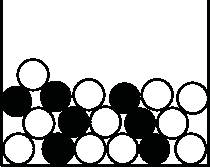
\includegraphics[width=0.3\linewidth]{Lect02/hypergeom.pdf}
				\caption{Гипергеометрическое распределение}
				\label{lect02:pic1}
			\end{figure}
            \item \emph{Пуассоновское распределение} $Pois(\lambda)$ --- число событий, произошедших за фиксированное время, при условии, что данные события происходят с некоторой фиксированной средней интенсивностью ($\lambda$) и независимо друг от друга. $\Omega = \{0, 1, 2, \dots \} \cong \mathbb{N} \cup \{0\}$.\\
            \begin{equation*}
                P\left(\{n\}\right) = \frac{\lambda^ne^{-\lambda}}{n!}
            \end{equation*}
        \end{enumerate}
    \subsection{Геометрические вероятности} 
        $P(A) := \frac{\mu(A)}{\mu(\Omega)}$.
        \begin{enumerate}
            \item \emph{Парадокс Бертрана}. Рассмотрим равносторонний треугольник, вписанный в окружность. Наудачу выбирается хорда окружности. Какова вероятность того, что выбранная хорда длиннее стороны треугольника?
            \begin{enumerate}
                \item \emph{Метод «случайного центра»}. Бросаем точку и проводим через нее хорду, перпендикулярную радиусу. Хорда длиннее стороны равностороннего треугольника, если выбранная точка находится внутри круга, вписанного в треугольник. $P = \frac{\pi{(\frac{R}{2})}^2}{\pi R^2} = \frac{1}{4}$.
                \item \emph{Метод «случайных концов»}. Фиксируем точку на окружности, берем произвольный угол $\alpha$. Чтобы посчитать искомую вероятность, представим, что треугольник повёрнут так, что одна из его вершин совпадает с концом хорды. Заметим, что если другой конец хорды лежит на дуге между двумя другими вершинами треугольника, то длина хорды больше стороны треугольника. Длина рассмотренной дуги равна трети длины окружности, значит, искомая вероятность равна $P = \frac{\frac{1}{3}(2 \pi R)}{2 \pi R} = \frac{1}{3}$.
                \item \emph{Метод «случайного радиуса»}. Случайно выбираем радиус, бросаем на радиус точку и строим через него хорду, перпендикулярную этому радиусу. Хорда длиннее стороны треугольника, если её центр ближе к центру, чем точка пересечения треугольника с зафиксированным радиусом, а сторона треугольника делит радиус пополам. $P = \frac{R}{2R} = \frac{1}{2}$.
            \end{enumerate}
            \begin{figure}[h!]
				\centering
				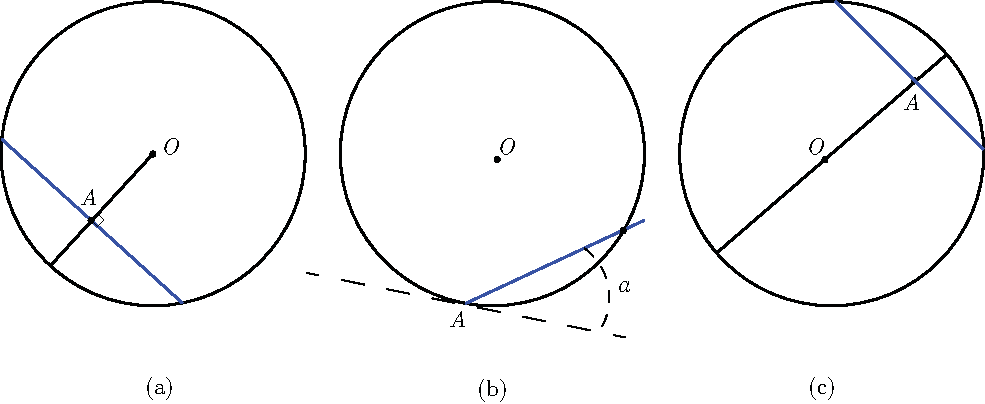
\includegraphics[width=0.6\linewidth]{Lect02/bertrand.pdf}
				\caption{Парадокс Бертрана. Синим отмечена полученная хорда}
				\label{lect02:pic2}
			\end{figure}
            Суть парадокса: проблема точной формализации эксперимента. Тогда и только тогда, когда метод случайного выбора задан, проблема имеет чётко определённое решение.
            \item \emph{Игла Бюффона}. Рассмотрим лист бумаги, расчерченный параллельными прямыми на $n$ полос длины $L$ и ширины $d$ ($|\Omega| = nd \cdot L$). Случайно бросаем на него иглу длиной $l < d$ (случайно выбираем центр $(x, y)$, затем случайно выбираем угол поворота $\alpha$). Какова вероятность того, что игла пересечет одну из линий решетки?\\
            Пусть центр $(x, y)$ оказался в полосе между $(k - 1)$-ой и $k$-ой линией, причем $y > (k - 1)d + \frac{d}{2}$ (случай, где центр находится ближе к $(k - 1)$-ой линии, симметричен). Тогда условие того, что игла, повернутая на угол $0 < \alpha < \pi$ пересекла $k$-ую линию:
            \begin{equation*}
                \begin{cases}
                    kd - \frac{d}{2} < y \leq kd\\
                    kd - y < \frac{l}{2}\sin\alpha
                \end{cases} \implies kd - \frac{l}{2}\sin\alpha < y \leq kd
            \end{equation*}
            Получаем $\int\limits_0^{\pi} (kd - (kd - \frac{l}{2}\sin\alpha))d\alpha = l$ --- для половины полосы.\\
            Искомая вероятность $\P = \frac{2l \cdot nL}{\pi d \cdot nL} = \frac{2l}{\pi d}$.
            \begin{figure}[h!]
				\centering
				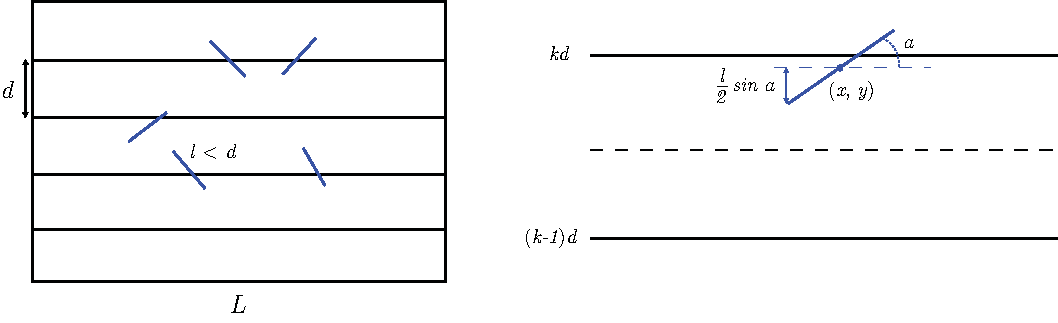
\includegraphics[width=0.9\linewidth]{Lect02/buffon.pdf}
				\caption{Игла Бюффона}
				\label{lect02:pic3}
			\end{figure}
        \end{enumerate}
    \subsection{Свойства вероятностной меры}
        \begin{theorem}\label{lect02:th1}
            Пусть $A, B \in \mathcal{F}$, \ $A_n \in \mathcal{F}$. Справедливы следующие утверждения:
            \begin{enumerate}
                \item $A \subseteq B \implies \P(B \setminus A) = \P(B) - \P(A)$, в частности, $\P(B) \geq \P(A)$
                \item $\P(A \cup B) = \P(A) + \P(B) - \P(AB)$
                \item \emph{(суббадитивность)} $\P(\bigcup\limits_n A_n) \leq \sum\limits_n \P(A_n)$
            \end{enumerate}
        \end{theorem}
        \begin{proof}
            \begin{enumerate}
                \item $B = A \sqcup (B \setminus A) = A \sqcup (B\overline{A})$. Т.к. $A(B \setminus A) = \varnothing$, то $\P(B) = \P(A) + \P(B \setminus A)$.
                \item \begin{equation*}
                    \begin{cases}
                        \P(A \cup B) = \P(A) + \P(B \setminus A)\\
                        \P(B) = \P(AB) + \P(B \setminus A)
                    \end{cases} \implies \P(A \cup B) = \P(A) + \P(B) - \P(AB)
                \end{equation*}
                \item $B_1 = A_1, \ B_2 = A_2 \setminus A_1, \ B_3 = A_3 \setminus (A_1 \cup A_2), \dots$\\
                $\bigsqcup\limits_i B_i = \bigcup\limits_i A_i \implies \P(\bigcup\limits_i A_i) = \P(\bigsqcup\limits_i B_i) = \sum\limits_i \P(B_i) \leq \sum\limits_i \P(A_i)$ (мажорируем ряд).
            \end{enumerate}
        \end{proof}
        \begin{theorem}\label{lect02:th2}
            Пусть $A_1, \dots, A_n \in \mathcal{F}$. Тогда $\P(\bigcup\limits_{i = 1}^n A_i) = \sum\limits_i \P(A_i) - \sum\limits_{i, j} \P(A_iA_j) + \sum\limits_{i, j, k} \P(A_iA_jA_k) - \dots + (-1)^{n - 1}\P(A_1\dots A_n)$.
        \end{theorem}
        \begin{proof}
            По индукции.
        \end{proof}
        \begin{definition}\label{lect02:def1}
             Неотрицательная функция $\mu: \mathcal{A} \implies \mathbb{R}$, $\mathcal{A} \subseteq 2^S$ --- алгебра, называется \emph{счетно-аддитивной}, если $\forall A_1, A_2, \dots \mathcal{A}: A_i \cap A_j = \varnothing \iff i \neq j$ и $\bigcup\limits_i A_i \in \mathcal{A}$ верно равенство $\mu(\bigcup\limits_i A_i) = \sum\limits_i \mu(A_i)$.
        \end{definition}
        \begin{definition}\label{lect02:def2}
             Неотрицательная функция $\mu: \mathcal{A} \implies \mathbb{R}$, $\mathcal{A} \subseteq 2^S$ --- алгебра, называется \emph{непрерывной в нуле}, если $\forall A_n \downarrow \varnothing$ при $n \implies \infty \implies \mu(A_n) \implies 0$ при $n \implies \infty$.
        \end{definition}
        \begin{lemma}\label{lect02:lemma1}
            Пусть $\mu$ --- неотрицательная конечно-аддитивная функция на $\mathcal{A}$ и $\forall A \in \mathcal{A} \ \mu(A) < \infty$. Тогда $\mu \in C(\varnothing) \implies \mu$ непрерывна на монотонных последовательностях: $A_n \downarrow (\uparrow) A$ при $n \implies \infty \implies \mu(A_n) \implies \mu(A)$ при $n \implies \infty$.
        \end{lemma}
        \begin{proof}
            $\forall A \in \mathcal{A} \ \mu(A) < \infty \iff \mu(S) < \infty$. Пусть $A_n \downarrow A \in \mathcal{A}$. Тогда $\mu(A_n \setminus A) \implies 0$ ($\mu$ непрерывна в нуле), а $\mu(A_n \setminus A) = \mu(A_n) - \mu(A) \implies \mu(A_n) \implies \mu(A)$.\\
            Для монотонно возрастающих последовательностей: положим $B_n = \overline{A_n}, B = \overline{A}$. Тогда $B_n \downarrow B \implies \mu(B_n) \implies \mu(B) \implies \mu(S) - \mu(A_n) \implies \mu(S) - \mu(A) \implies \mu(A_n) \implies \mu(A)$ при $n \implies \infty$.
        \end{proof}
        \begin{theorem}\label{lect02:th3}
            Пусть $\mu$ --- конечная неотрицательная функция, заданная на алгебре $\mathcal{A}$ подмножеств $S$. Тогда $\mu$ счетно-аддитивна тогда и только тогда, когда $\mu$ конечно-аддитивна и непрерывна в нуле.
        \end{theorem}
        \begin{proof}
            $\implies$. Пусть $\mu$ счетно-аддитивна, тогда она, очевидно, является конечно-аддитивной. Покажем ее непрерывность в нуле: $A_n \in \mathcal{A} \downarrow \varnothing$. Положим $B_n = A_n \setminus A_{n + 1}$. Очевидно, что $B_iB_j = \varnothing$ при $i \neq j$. Заметим, что $A_n = \bigcup\limits_{k = n}^{\infty}B_k$. $A_1 = \bigcup\limits_{k = 1}^{\infty}B_k \implies \mu(A_1) = \sum\limits_{k = 1}^{\infty} \mu(B_k)$ в силу счетной аддитивности $\mu$. Поскольку ряд сходится, $\mu(A_n) \implies 0$ при $n \implies \infty$.\\
            $\impliedby$. Возьмем $C_k \in \mathcal{A} : C_iC_j = \varnothing$ при $i \neq j$, $\bigcup\limits_k C_k \in \mathcal{A}$. Положим $A_n = \bigcup\limits_{k = n}^{\infty} C_k$. Очевидно, что $A_1 = C_1 \cup C_2 \cup \dots \cup C_{n - 1} \cup A_n$, $n \geq 2 \implies A_n = A_1 \setminus (C_1 \cup \dots \cup C_{n - 1}) \in \mathcal{A}$, причем $C_1, \dots C_{n - 1}, A_n$ попарно не пересекаются.\\
            Очевидно, что $A_n \downarrow \varnothing$ и из конечной аддитивности $\mu(A_1) = \mu(C_1) + \dots + \mu(C_{n - 1} + \mu(A_n))$. Из непрерывности в нуле: $\mu(A_n) \implies 0 \implies \sum\limits_{k = 1}^n \mu(C_k) \implies \mu(A_1) = \mu(\bigcup\limits_{k = 1}^{\infty} C_k) \implies \sum\limits_{k = 1}^n \mu(C_k) = \mu(\bigcup\limits_{k = 1}^{\infty} C_k)$. 
        \end{proof}
        \begin{theorem}\label{lect02:th4}
            Пусть $P, Q$ --- вероятностные меры, заданные на измеримом пространстве $(S, \mathcal{B})$, совпадающие на $\pi$-системе $\mathcal{M}$. Тогда они совпадают на $\sigma (\mathcal{M})$. 
        \end{theorem}
        \begin{proof}
            Положим $\mathcal{D} = \{ A \in \mathcal{B}: P(A) = Q(A)\}$. Тогда по условию теоремы $\mathcal{M} \subseteq \mathcal{D}$. Заметим, что
            \begin{enumerate}
                \item $S \in \mathcal{D}$, т.к. $P(S) = Q(S) = 1$.
                \item $A, B \in \mathcal{D}, \ A \subseteq B \implies B \setminus A \in \mathcal{D}$, т.к. $P(B \setminus A) = P(B) - P(A) = Q(B) - Q(A) = Q(B \setminus A)$.
                \item $A_n \in \mathcal{D}$, $A_n \uparrow A \implies A \in \mathcal{D}$, т.к. $0 = \lim\limits_{n \implies \infty} 0 = \lim\limits_{n \implies \infty} P(A_n) - Q(A_n) = P(A) - Q(A) \implies P(A) = Q(A) \implies A \in \mathcal{D}$ (из непрерывности вероятности).
            \end{enumerate}
            Значит, $\mathcal{D}$ является $\lambda$-системой. По теореме \ref{lect01:th2} $\mathcal{D} = \sigma (\mathcal{M})$.
        \end{proof}
        \begin{theorem}\label{lect02:th5}
            \emph{(Каратеодори)}. Любая вероятностная мера на алгебре $\mathcal{A} \subseteq 2^S$ однозначно продлевается на $\sigma (\mathcal{A})$.
        \end{theorem}
        \begin{proof}
            (схема)
            \begin{enumerate}
                \item Определим внешнюю меру следующим образом: $P^* (A) = \inf \{ \sum\limits_n \P(A_n): A_n \in \mathcal{A}, A \subseteq \bigcup\limits_n A_n \}$. 
                \item Из теоремы \ref{lect02:th1} следует, что можно обойтись покрытиями, состоящими из попарно непересекающихся множеств $A_n \in \mathcal{A}$.
                \item \emph{Оказывается}, что $P^*|_{\mathcal{A}} \equiv P$.
                \item $\forall A, B \in 2^S \ \rho (A, B) = P^*(A \bigtriangleup B)$.
                \item Положим $\mathcal{A}^* = \{ A \in 2^S: \exists A_n \in \mathcal{A} \rho (A_n, A) \implies 0 \text{ при } n \implies \infty \}$. \emph{Очевидно}, что $\mathcal{A} \subseteq \mathcal{A}^*$. 
                \item \emph{Проверяется}, что $\mathcal{A}^*$ --- $\sigma$-алгебра.
                \item \emph{Доказывается}, что $(S, \mathcal{A}^*, P^*)$ --- вероятностное пространство.
            \end{enumerate}
            Единственность продления следует из теоремы \ref{lect02:th4}, т.к. алгебра есть $\pi$-система.
        \end{proof}
	\section{Условные вероятности}
	
	\subsection{Вероятностные меры на $(\mathbb{R},\mathcal{B}(\mathbb{R}))$. Примеры распределений}
	
	\begin{definition}\label{lect03:def1}
	Пусть $P$ -- вероятностная мера на $(\mathbb{R},\mathcal{B}(\mathbb{R}))$. Её функцией распределения назовём функцию $F(x):=P((-\infty,x]), x\in\mathbb{R}$.
	\end{definition}
	
	\begin{theorem}\label{lect03:th1}
	Пусть $F$ -- функция распределения. Тогда $F$ обладает следующими свойствами:
	    \begin{enumerate}
	        \item $F$ не убывает на $\mathbb{R}$
	        \item $F$ непрерывна справа в каждой точке
	        \item $\lim\limits_{x\to -\infty}{F(x)} = 0$
	        \item $\lim\limits_{x\to +\infty}{F(x)} = 1$
	    \end{enumerate}
	\end{theorem}
	\begin{proof}
	    \begin{enumerate}
	        \item Очевидно: если $x\le y$, то $(-\infty,x]\subset (-\infty,y]$. Осталось вспомнить теорему \ref{lect02:th1}.
	        \item Если $x_n\downarrow x$, то $(-\infty,x_n]\downarrow(-\infty,x]$, и по непрерывности вероятностной меры получаем $F(x_n)\to F(x)$.
	        \item Рассмотрим $B_n=(-\infty,x_n]$. Если $x_n\downarrow -\infty$, то $B_n\downarrow\varnothing$, и\\ $\lim_{n\to\infty}F(x_n)=\lim_{n\to\infty}{P(B_n)}=P(\varnothing)=0$.
	        \item Аналогично пункту 3, только теперь берём $x_n\uparrow +\infty$.
	    \end{enumerate}
	\end{proof}
	
	\begin{theorem}\label{lect03:th2}
	    Пусть $F$ обладает свойствами из \ref{lect03:th1}. Тогда на $(\mathbb{R},\mathcal{B}(\mathbb{R}))$ существует единственная вероятностая мера $P$, для которой $F$ является функцией распределения.
	\end{theorem}
	\begin{proof}
	    Допустим, что нашлась такая $P$, для которой $F$ является функцией распределения. Тогда $P((a,b])=P((-\infty,b]\setminus (-\infty,a]) = F(b)-F(a)$.

	    Пусть $A=\bigcup\limits_{k=1}^{m} (a_k,b_k]$, $(a_i,b_i]\cap (a_j,b_j] = \varnothing$ при $i\neq j$ (допускаем бесконечные промежутки). Тогда $P(A)=\sum\limits_{k=1}^{m} P((a_k,b_k]) = \sum\limits_{k=1}^{m}(F(b_k)-F(a_k))$. Легко видеть, что множества, на которых мы только что определили меру $P$, образуют алгебру подмножеств на прямой $\mathcal{A}$, и $P(A)$ не зависит от вида представления $A$ в виде объединения. 
	    
	    Напоминание(\ref{lect02:th3}): $P$ на $\mathcal{A}$ сигма-аддитивна $\iff$ конечно-аддитивна и непрерывна в $\varnothing$. Конечная аддитивность очевидна. Проверим, что она непрерывна в $\varnothing$. Тогда $P$ будет вероятностной на $\mathcal{A}$.
	    
	    Пусть $A_n = \bigcup\limits_{k=1}^{m_n} (a_k^{(n)},b_k^{(n)}], A_n\downarrow\varnothing$. Докажем, что $\lim_{n\to\infty}P(A_n) = 0$.
	    
	    По свойствам 3 и 4 функции распределения (\ref{lect03:th1}) имеем $\forall\eps>0 \\ \exists a=a(\eps), b=b(\eps): F(a)<\frac{\eps}{2}, F(b)>1-\frac{\eps}{2}$. Тогда $P(\mathbb{R}\setminus (a,b]) = F(a)+1-F(b)<\eps$.
	    
	    $P(A_n) = P(A_n \cap (\mathbb{R} \setminus (a,b])) + P(A_n \cap (a,b])$. В предыдущей строчке написано, что первое слагаемое меньше $\eps$.
	    
	    Без ограничения общности считаем, что $A_n\downarrow\varnothing$, а также $\forall n$ $A_n\subset (a,b]$. Будем рассматривать только $A_n\neq\varnothing$.
	    
	    Итак, $A_n = \bigcup\limits_{k=1}^{m_n} (a_k^{(n)},b_k^{(n)}]$. Рассмотрим $B_n = \bigcup\limits_{k=1}^{m_n} (x_k^{(n)},b_k^{(n)}]$, где $x_k^{(n)}$ выбраны так, что $a_k^{(n)}<x_k^{(n)}<b_k^{(n)}$ и $F(x_k^{(n)})-F(a_k^{(n)})<\frac{2^{-n}\eps}{m_n}$ (это возможно в силу того, что $F$ непрерывна справа). Ещё рассмотрим $C_n = \bigcup\limits_{k=1}^{m_n} [x_k^{(n)},b_k^{(n)}]$. Очевидно, $C_n$ замкнуто, $C_n\subset A_n$ и $P(A_n)-P(C_n)\le \sum\limits_{k=1}^{m_n} \frac{2^{-n}\eps}{m_n} = 2^{-n}\eps$. $ \bar C_n := \mathbb{R}\setminus C_n$ открыто. $\bigcap\limits_{n=1}^{\infty} C_n \subset \bigcap\limits_{n=1}^{\infty} A_n = \varnothing$, значит, $\bigcup\limits_{n=1}^{\infty} \bar C_n \supset \bar \varnothing = \mathbb{R}$. $\bigcup\limits_{n=1}^{\infty} \bar C_n \supset [a,b]$, значит, $\exists n_1<\ldots<n_r: [a,b] \subset \bar C_{n_1} \cap \ldots \cap \bar C_{n_r}$, а тогда $ C_{n_1} \cap \ldots \cap C_{n_r} \subset \overline{[a,b]}$. Но $\forall i$ $C_{n_i}\subset [a,b]$, значит, $C_{n_1} \cap \ldots \cap C_{n_r} = \varnothing$. 
	    
	    $P(A_{n_r}) = P\left(A_{n_r} \setminus \bigcup\limits_{j=1}^{r} C_{n_j}\right) = P\left(A_{n_r}\cap \overline{\bigcup\limits_{j=1}^{r} C_{n_j}} \right) = P\left(A_{n_r}\cup\bigcup\limits_{j=1}^{r}{\bar C_{n_j}} \right) \le \sum\limits_{j=1}^{r} P(A_{n_r} \cap \bar C_{n_j}) \le \sum\limits_{j=1}^{r} P(A_{n_j}\cap \bar C_{n_j}) \le \eps (\sum\limits_{j=1}^{r} 2^{-n_j}) \le \eps$. 
	    
	    Итак, всё. Доказали, что $\lim_{n\to\infty}P(A_n) = 0$, и получили, что мера является сигма-аддитивной. Осталось заметить, что по теореме Каратеодори меру можпо однозначно продолжить с $\mathcal{A}$ на $\sigma \{\mathcal{A}\}=\mathcal{B}(\mathbb{R})$.
	\end{proof}
	
	\begin{definition}\label{lect03:def2}
	    Функция $p(x)$ называется плотностью, если $p(x)\ge 0$ $\forall x\in\mathbb{R}$ и $\int\limits_{-\infty}^{+\infty} p(x)dx = 1$.
	\end{definition}
	
	\begin{prop}\label{lect03:prop1}
	Возьмём $F(x) = \int\limits_{(-\infty,x]}p(u)du$. Тогда $F$ обладает свойствами 1-4 из \ref{lect03:th1}, и следовательно является функцией распределения некоторой вероятностной меры. 
	\end{prop}
	
	\begin{example}
	    Равномерное распределение на отрезке $[a,b]$ $$p(x)=\frac{1}{b-a}\cdot\1([a,b])$$
	\end{example}
	
	\begin{example}
	    Экспоненциальное распределение с параметром $\lambda >0$
	    $$p(x)=\lambda e^{-\lambda x}\cdot\1([0,+\infty))$$
	\end{example}
	
	\begin{example}
	    Распределение Коши
	    $$p(x)=\frac{1}{\pi (1+x^2)}$$
	\end{example}
	
	\begin{example}
	    Распределение Парето с параметром $a>0$
	    $$p(x)=\frac{1}{ax^{a+1}}\cdot\1([1,+\infty))$$
	\end{example}
	
	\begin{example}
	    Гауссовское (нормальное) распределение $\mathcal{N}(a,\sigma)$ с параметрами $a\in\mathbb{R}$ и $\sigma >0$
	    
	    $$p(x) = \frac{1}{\sigma\sqrt{2\pi}}e^{-\frac{(x-a)^2}{2\sigma^2}}$$
	\end{example}
	\begin{definition}
		$\mathcal{N}(0,1)$ -- стандартное нормальное распределение.
	\end{definition}
	
	\subsection{Пополнение вероятностного пространства. Мера Лебега}
	
	\begin{definition}\label{lect03:def3}
	Пусть $(\Omega,\mathcal{F},P)$ -- вероятностное пространство. Пусть $\mathcal{N} = \{B\subset\Omega: \exists A: A\supset B, P(A)=0\}$. Тогда пополнением $\mathcal{F}$ назовём $\mathcal{\bar F} = \{ A \cup B: A \in \mathcal{F} , B \in \mathcal{N} \}$. Это то же самое, что и $\sigma\{\mathcal{F},\mathcal{M}\}$. Пополнением вероятностного пространства назовём $(\Omega,\mathcal{\bar F},\bar P)$, где $\bar P$ определена на $\mathcal{\bar F}$ следующим образом: $\bar P(C) = P(A)$, если $C=A\cup B$, где $A\in\mathcal{F},B\in\mathcal{N}$.
	\end{definition}
	
    Упражнение. Проверить корректность определения, т.е. что если \\$A,A'\in\mathcal{F}, B,B'\in\mathcal{N}$ и $A\cup B = A' \cup B'$, то $\bar P(A\cup B) = \bar P(A' \cup B')$.
    
    \begin{definition}\label{lect03:def4}
        Мера $\mu$ на $(S,\mathcal{B})$ называется $\sigma$-конечной, если существует счётный набор множеств $\{ S_n\}$ такой, что $\mu (S_n)\le \infty$ и $S=\bigcup\limits_{n=1}^{\infty} S_n$.
    \end{definition}
    
    \begin{definition}\label{lect03:def5}
    Пусть $B\in\mathcal{B}(\mathbb{R})$. Тогда $B = \bigcup\limits_{n\in\mathbb{Z}} (B\cap (n,n+1])$. Введём $\mu_n$ - равномерное распределение на $(n,n+1]$. Тогда определим $\mu(B) = \sum\limits_{n\in\mathbb{Z}} \mu_n(B\cap (n,n+1])$. Это мера Лебега.
    \end{definition}
    
    \subsection{Условная вероятность}
    
    \begin{definition}\label{lect03:def6}
        Пусть $(\Omega,\mathcal{F},P)$ -- вероятностное пространство, ${P(B)>0}$. Условной вероятностью события $A$ при условии $B$ назовём 
        $$
        P(A|B) := \frac{P(A\cap B)}{P(B)}
        $$
    \end{definition}
    
    \begin{theorem}(Формула полной вероятности)\label{lect03:th3}
        Пусть $\Omega = B_1 \sqcup \ldots \sqcup B_n \sqcup \ldots $. Тогда $P(A) = \sum_{j} P(AB_j) = \sum_{j} P(A|B_j)P(B_j)$.
    \end{theorem}
	\section{Независимость событий}

\begin{example}\label{lect04:ex1}
	Студент из $N$ билетов выучил $n$. Перед ним $k$ человек. Какова вероятность, что студент вытащил "хороший"\, билет (то есть тот, который выучил)?
	
	
	$A = \{$студент вытащил хороший билет$\}$
	
	Ответ: $P(A) = \frac{n}{N}$.
\end{example}

\begin{theorem}\label{lect04:th1} Формула Байеса
	
	
	$ \Omega = \bigsqcup \limits_{i} B_i$, $P(B_i) > 0$ $\forall i$ $\implies \forall k$ $P(B_k \vert A) = \frac{P(A \vert B_k) P(B_k)}{\sum \limits_{i}  P(A\vert B_i) P(B_i)}$
\end{theorem}
\begin{proof}
	следствие формулы полной вероятности: 
	
	$$P(B_k \vert A) = \frac{P(AB_k)}{P(A)} = \frac{P(A \vert B_k) P(B_k)}{\sum \limits_{i}  P(A\vert B_i) P(B_i)}$$
\end{proof}
\begin{example}\label{lect04:ex2}
	При рентгеновском обследовании вероятность обнаружить заболевание N у больного равна 0.95, вероятность принять здорового человека за больного равна 0.05. Доля больных по отношению ко всему населению равна 0.01. Найти вероятность того, что человек здоров, если он был признан больным при обследовании. 
	
	
	\textit{Решение.}  Предположим, что:\\
	$A = $\{человек здоров\}, $B = $\{человек болен\},\\
	$B_1 =$ \{обнаружили заболевание\}, $B_2 =$\{не обнаружили заболевание\}.\\
	Тогда из условия получаем: 
	$$P(B_1 \vert B)=0.95,\, P(B_1 \vert A)=0.05,\, P(B)=0.01,\, P(A)=0.99.$$
	Вычислим полную вероятность признания больным:
	$$P(B_1) = P(B_1 \vert A)P(A)+P(B_2 \vert B)P(B) =  0.99 \cdot 0.05+0.01\cdot0.95=0.059.$$
	Вероятность «здоров» при диагнозе «болен» можно посчитать, применив формулу Байеса:
	$$P(A \vert B_1) =\frac{P(A)P(B_1 \vert A)}{P(A)P(B_1 \vert A) + P(B)P(B_1 \vert B)} = \frac{0.99 \cdot 0.05}{(0.99 \cdot 0.05+0.01\cdot 0.95}=0.839.$$
	
	Таким образом, $83.9\%$ людей, у которых обследование показало результат «болен», на самом деле здоровые люди. Удивительный результат возникает по причине значительной разницы в долях больных и здоровых. Болезнь $N$ — редкое явление, поэтому и возникает такой парадокс Байеса. При возникновении такого результата лучше всего сделать повторное обследование.
\end{example}
\begin{definition}\label{lect04:def1}
	Событие $A$ \textit{не зависит} от $B$, если $P(A \vert B) = P(A)$ (предполагается, что $P(B) \neq 0$).
\end{definition}
\begin{definition}\label{lect04:def2}
	События $A$ и $B$ \textit{независимые} (или $A$ не зависит от $B$ и  $B$ не зависит от $A$), если $P(AB) = P(A)P(B)$.
\end{definition}

\begin{prop}\label{lect04:prop1}
	A не зависит от B тогда и только тогда когда A и B независимы или B невероятно.
	%%как тут сформилировать утверждение???
\end{prop}
\begin{proof}
	$$
	\begin{array}{rcl}
	P(A \vert B) & = &  P(A) \\
	P(A \vert B)  & = & \frac{P(AB)}{P(B)} 
	\end{array} \iff P(A) = \frac{P(AB) }{P(B)} \iff P(AB) = P(A)P(B) $$
\end{proof}


\begin{example}\label{lect04:ex3}
	Из колоды, содержащей 36 карт, наудачу вынимается одна карта. 
	Пусть $A =$ \{достали туз\},  $B =$ \{достали карту трефовой масти $\clubsuit$\}.  Можно ли утверждать, что данные события независимы?
	
	
	\textit{Решение.}
	Из условия имеем: $|\Omega| = 36, \, |A| = 4, \, |B| = 9, \, |AB| = 1$.
	
	$$P(A) = \frac{4}{36} = \frac{1}{9}, \, P(B) = \frac{9}{36} = \frac{1}{4}, \, P(AB) = \frac{1}{36}$$
	Получаем, что $P(AB) = P(A)P(B) \implies$ по определению события независимы.
\end{example}
\begin{definition}\label{lect04:def3}
	События $A_z, \, z \in T$ называются \textit{попарно независимыми}, если $\forall s \neq t \in T$ $P(A_sA_t) = P(A_s)P(A_t).$
\end{definition}
\begin{definition}\label{lect04:def4}
	События $A_z, \, z \in T$ называются \textit{независимыми в совокупности}, если $\forall U \subset T$ $(|U| < |\infty|):$ $P(\bigcap \limits_{t\in U} A_t) = \prod \limits_{t\in U} P(A_t).$     
	
\end{definition}

\begin{example}\label{lect04:ex4}События попарно независимы, но зависимы с совокупности:
	Пусть $\Omega = \{1, 2, 3, 4\}, \, A_1 = \{1, 2\}, \, A_2 = \{1, 3\}, \, A_3 = \{1, 4\}.$\\
	Тогда $P(A_i) = \frac{2}{4} = \frac{1}{2}\,$ $\forall i = 1, \dots , 3$ и $P(A_iA_j) = \frac{1}{4}, \, i \neq j$.
	
	Получаем, что $P(A_iA_j) = \frac{1}{4} = \frac{1}{2} \cdot \frac{1}{2} = P(A_i)P(A_j) \implies$ события попарно независимы.\\
	$P(A_1A_2A_3) = \frac{1}{4} \neq \frac{1}{8} = P(A_1)P(A_2)P(A_3) \implies$ события зависимы в совокупности.
\end{example}

\begin{example}\label{lect04:ex5}  Пример Бернштейна 
	
	
	Рассмотрим правильный тетраэдр, три грани которого окрашены соответственно в красный, синий, зелёный цвета, а четвёртая грань содержит все три цвета. \\
	$A_1 = $  \{выпала грань, содержащая красный цвет\},\\
	$A_2 = $ \{выпала грань, содержащая синий цвет\},\\
	$A_3 = $ \{выпала грань, содержащая зеленый цвет\}.
	
\end{example}

\begin{lemma}\label{lect04:lemma1}
	Пусть $A_1, \dots, A_n$ $(n \geq 2)$ независимы в совокупности и $B_k = A_k$ или $A_k^C$ при $k = 1, \dots, n$. Тогда $B_1, \dots, B_n$ - независимые события.
\end{lemma}     
\begin{proof}
	Достаточно рассмотреть случай, когда $B_i = A_i^C$ и $B_k = A_k \, \forall k\neq i$. Проверим определение:  \\
	$U \subseteq \{1, \dots n \}$\\
	$S := \{1, \dots n\} \setminus U$\\
	$i \notin U \implies P(\bigcap \limits_{j \in U} B_j) = \prod \limits_{j \in U} P(B_j)$, потому что каждое $B_i = A_i$, а  $A_i$ - независимы в совокупности.\\
	$i \in U \implies P(\bigcap \limits_{j \in U} B_j) = P(\bigcap \limits_{j \in S} A_j) - P(A_i \cap (\bigcap \limits_{j \in S} A_j)) = P(\bigcap \limits_{j \in S} A_j) - P(A_i)P(\bigcap \limits_{j \in S} A_j)) = \prod \limits_{j \in S}P(A_j) - P(A_i) \prod \limits_{j \in S} P(A_j) = (1- P(A_i))\prod \limits_{j \in S} P(A_j) = P(A_i^C)\prod \limits_{j \in S} P(A_j) = \prod \limits_{j \in U} P(B_j)$
\end{proof}

\begin{theorem}\label{lect04:th2} Формула Эйлера из теории чисел
	
	Пусть $\phi : \N \to \N, \, n \mapsto \phi(n)$ - количество чисел $k \in \{1, \dots, n\}$, которые  взаимно простых с $n$. Тогда $\phi(n) = n \prod \limits_{p \in J_n} (1 - \frac{1}{p})$, где $J_n$ - множество всех простых делителей n (другими словами, если $n = p_1^{k_1} \dots p_m^{k_m}$, где простые числа $p_1 < \dots < p_m$ и $k_i \geq 1$ $i = 1, \dots, m$, $J_n = \{p_1, \dots, p_m\}$.
\end{theorem}    
\begin{proof}
	Введём $\Omega = \{1, \dots, n\}$, $\mathcal{F} = 2^\Omega$, пусть выполнено классическое определение вероятности $P(\{i\}) = \frac{1}{n}$ при $i = 1, \dots, n$ (можно сказать, что рассматривается случайный эксперимент, в котором наудачу выбирается одно число из множества от 1 до $n$).\\
	Пусть событие $A = \{$выбранное число взаимно просто с $n$\}. Тогда $P(A) = \frac{\phi(n)}{n}$. \\
	Введём событие $A_i =$\{выбранное число делится на $p_i$\} $= \{p_i, 2p_i, \dots, \frac{n}{p_i}p_i\}$, $|A_i| = \frac{n}{p_i}$, поэтому $P(A_i) = \frac{\frac{n}{p_i}}{n} = \frac{1}{p_i}$ для $i = 1, \dots, m$. \\
	Тогда $A_{i_1}\dots A_{i_k} =\{p_{i_1}\dots p_{i_k}, 2p_{i_1}\dots p_{i_k}, \dots, \frac{p_{i_1}\dots p_{i_k}}{n}p_{i_1}\dots p_{i_k}\}$ $(1 \leq i_1 < \dots < i_k \leq m) \implies P(A_{i_1}\dots A_{i_k}) = \frac{1}{p_{i_1}\dots p_{i_k}} = P(A_{i_k})\dots P(A_{i_k})$, то есть события $A_{i_1}, \dots, A_{i_k}$ - независимы.
	
	
	
	
	$$P(A) = P((\bigcup \limits_{i=1}^m A_i)^C) = P(\bigcap \limits_{i=1}^m A_i^C) \overset{\makebox[25pt]{\mbox{\normalfont\tiny по лемме}}}{=} \prod \limits_{i=1}^m P(A_i^C) = \prod \limits_{i=1}^m  (1 - P(A_i)) = \prod \limits_{i=1}^m (1 -\frac{1}{p_i})$$
\end{proof}


\begin{definition}\label{lect04:def5}
	Пусть даны системы событий $\mathcal{A}_t \subset \mathcal{F},\, t \in T$, где $T$ некоторое множество $|T| \geq 2$. Эти \textit{системы независимы в совокупности}, если для любого конечного $U \subset T$ независимы события $A_t \in \mathcal{A}_t, \, t \in U $.
\end{definition}

\begin{theorem}\label{lect04:th3}
	Пусть независимы $\pi-$системы $\mathcal{A}_t \subset \mathcal{F}, \, t \in T$, где $\mathcal{F}$ - это $\sigma-$алгебра. Тогда независимы  $\sigma \{\mathcal{A}_t\}$ $\sigma-$алгебры, порождённые этими системами.
\end{theorem}    
\begin{proof}
	Возьмём $\forall \{t_1, \dots, t_n \} \subset T$ и $A_{t_k} \in \mathcal{A}_{t_k}, \, k = 1, \dots, n$. Введём систему  $\mathcal{K}_{t_1}$, состоящую из событий $B$ таких, что $P(B A_{t_2}\dots A_{t_n}) = P(B)P(A_{t_2})\dots P(A_{t_m})$. 
	
	Легко увидеть, что $\mathcal{K}_{t_1}$ - это $\lambda$-система: 
	\begin{itemize}
		\item $\Omega \in \mathcal{K}_{t_1}$;
		\item $A, B \in \mathcal{K}_{t_1}, A\subseteq B \overset{?}{\implies} B \setminus A \in        \mathcal{K}_{t_1}$\\
		$P(B\dots A_{t_n}) - P(A\dots A_{t_m}) = (P(B) - P(A))P(A_{t_2})\dots P(A_{t_n}) = $\\
		$ = P(B\setminus A)P(A_{t_2})\dots P(A_{t_n}) = P((B\setminus A)A_{t_2} \dots A_{t_n})$;
		\item Следует из непрерывности меры.
	\end{itemize}
	
	По теореме о $\pi$-$\lambda$ - системах получаем, что $\sigma \{\mathcal{A}_{t_1} \} \subset \mathcal{K}_{t_1}$. Следовательно, соотношение $P(B A_{t_2}\dots A_{t_n}) = P(B)P(A_{t_2})\dots P(A_{t_m})$ верно для $\forall B \in \sigma\{\mathcal{A}_{t_1} \}$.
	
	
	Продолжая аналогичным образом, приходим к равенству $P(A_{t_1}\dots A_{t_n}) = P(A_{t_1})\dots P(A_{t_n})$ для $\forall A_{t_k} \in \sigma \{\mathcal{A}_{t_k} \}$.
\end{proof}


\begin{lemma}\label{lect04:lemma2} (о группировке)
	
	Пусть $\mathcal{A}_{t}, t \in T -$ семейство независимых $\sigma$-алгебр (то есть $\forall t \, \mathcal{A}_{t} \subset \mathcal{F}$). Возьмём $\Lambda \subset T$ такое, что $\Lambda = \bigsqcup \limits_{\alpha \in \Gamma} \Lambda_{\alpha}$. Определим $\mathcal{F}_{\alpha} = \sigma \{\mathcal{A}_t, \, t \in  \Lambda_{\alpha}\}$. Тогда $\mathcal{F}_{\alpha}, \, \alpha \in \Gamma$ - семейство независимых $\sigma$-алгебр.
\end{lemma}     
\begin{proof}
	$\forall n \in \N$ $\forall \alpha_1, \dots, \alpha_n \in \Gamma$\\
	$B_{\alpha_1} \in \mathcal{F}_{\alpha_1}, \dots, B_{\alpha_n} \in \mathcal{F}_{\alpha_n}$\\
	$P(B_{\alpha_1} \dots B_{\alpha_n}) \overset{?}{=} P(B_{\alpha_1})\dots P(B_{\alpha_n})$
	
	
	Пусть $\mathcal{F}_{\alpha_1} = \sigma \{\mathcal{A}_t, \, t \in  \Lambda_{\alpha_1}\}$, тогда $\mathcal{F}_{\alpha_1} = \sigma \{\overbrace{\mathcal{A}_{t_1} \cap \dots \cap \mathcal{A}_{t_m}}^{\makebox[32pt]{\mbox{\normalfont\tiny система из таких - $\pi$-система (обозн. $M_{\alpha_1}$)}}} | \forall t_1, \dots, t_m \in \Lambda_{\alpha_1} \}$ 
	
	
	
	$P(\overbrace{A_{t_1} \dots A_{t_n}}^{\in M_{\alpha_1}} \overbrace{B_{s_1} \dots B_{s_q}}^{\in M_{\alpha_2}}  \dots) = P(A_{t_1})\dots P(A_{t_m}) P(B_{s_1})\dots P(B_{s_q}) \dots =$\\
	$= P(A_{t_1}\dots A_{t_m}) P(B_{s_1} \dots B_{s_q}) \dots \implies \{M_{\alpha_i}\} - $ независимые $\pi$-системы $\implies$ незавимое семейство $\sigma$-алгебр, порожденных $\pi$-системами.  
	
\end{proof}


\begin{lemma}\label{lect04:lemma3} (Борель-Кантели)
	
	Пусть $A_n$ - последовательность событий
	\begin{enumerate} 
		\item Если $\sum P(A_k) < \infty$, то $P($произойдёт бесконечное число $A_k$-ых$) = 0$ 
		
		(или $P( \bigcap \limits_{n=1}^{\infty} \bigcup \limits_{k \geq n}^{\infty} A_k) = P(\lim \sup A_k)$).
		\item Если $A_1, A_2, \dots$ - независимы, то $P($произойдёт бесконечное число $A_k$-ых$) = 1$,
	\end{enumerate}
\end{lemma}        
\begin{proof}
	\begin{enumerate} 
		\item $A \subset \bigcup \limits_{k \geq n} A_k \, \forall n$, $A = \lim \sup A_k$\\
		$0 \leq P(A) \leq P(\bigcup \limits_{k \geq n} A_k) \leq \sum \limits_{k=n}^{\infty} P(A_k) \to 0$
		\item Проверим, что $P((\lim \sup A_k)^C) = 0$\\
		$A^C = (\bigcap \limits_{n=1}^{\infty} \bigcup \limits_{k \geq n}^{\infty} A_k)^C = \bigcup \limits_{n=1}^{\infty} \bigcap \limits_{k \geq n}^{\infty} A_k^C = \lim \inf A_k^C$\\
		$P(A^C) \leq \sum \limits_{n=1}^{\infty}P(\bigcap \limits_{k \geq n} A_k^C)$ (субаддитивность)\\
		Фиксируем $n \in \N$. $P(\bigcap \limits_{k=n}^N A_k^C) \xrightarrow{N \to \infty} P(\bigcap \limits_{k=n}^{\infty} A_k^C)$ по непрерывности вероятностной меры.\\
		$P(\bigcap \limits_{k=n}^N A_k^C) = \prod \limits_{k=n}^N P(A_k^C)$ - из леммы $\{A_n, \dots, A_N\}$ - независимы $\implies \{A_n^C, \dots, A_N^C\}$ - независимы.\\
		$P(\bigcap \limits_{k=n}^N A_k^C) = \prod \limits_{k=n}^N P(A_k^C) = \prod \limits_{k=n}^N (1-P(A_k)) \overset{\makebox[30pt]{\mbox{\normalfont\tiny $1-x \leq e^x$}}}{\leq}  \prod \limits_{k=n}^N e^{-P(A_k)}=$\\
		$ = e^{-\sum \limits_{k=n}^N P(A_k)}  \xrightarrow{N \to \infty} 0$ (так как ряд расходится).
	\end{enumerate}
\end{proof}
	\section{Случайные величины и их распределения}

\subsection{Случайные элементы}
\begin{definition}\label{lect05:def1}
	Пусть $(V, \mathcal{A}), \,(S, \mathcal{B})$ - некоторые измеримые пространства. Отображение $f: V \to S$ называется \textit{$\mathcal{A} | \mathcal{B}$-измеримым}, если $\forall B \in \mathcal{B} \, f^{-1}(B) \in \mathcal{A}$, то есть $f^{-1}(\mathcal{B}) \subseteq \mathcal{A}$.
	
	Если  $(V, \mathcal{A}) = (\Omega, \mathcal{F})$ и $X \in \mathcal{F}|\mathcal{B}$, то $X$ называют \textit{случайным элементом}.
	
	Если $S = \R^n, \, \mathcal{B} = \mathcal{B}(\R^n), \, X:(\Omega, \mathcal{F}, P) \to (\R^n, \mathcal{B}(\R^n))$, то $X$ называется 
	\begin{enumerate}
		\item $n = 1$ при \textit{случайной величиной};
		\item $n > 1$ при \textit{случайным вектором}.
	\end{enumerate}
\end{definition}

\begin{example}\label{lect05:ex1}
	Индикатор $\1_A(x) = 
	\begin{cases}
	1, \, x \in A\\
	0, \, x \notin A\\
	\end{cases}\,$ - случайная величина, так как $\1^{-1}(\{1\}) = A \in \mathcal{F}$ и  $\1^{-1}(\{0\}) = A^C \in \mathcal{F}$.        
\end{example}

\begin{lemma}\label{lect05:lemma1}
	Пусть $f: V \to S$. Возьмём в $S$ произвольную систему подмножеств $M$ и рассмотрим в $V$ систему $ f^{-1}(M)$. Введём $\mathcal{B} := \sigma \{M\}$, $\mathcal{A} := \sigma\{f^{-1}(M)\}$. Тогда $f \in \mathcal{A}|\mathcal{B}$. Более того, $\sigma \{ f^{-1}(M)\} = f^{-1}(\sigma\{M\})$.
\end{lemma}
\begin{proof}\,
	
	\fbox{$\supset$}
	Определим $\mathcal{D}:= \{B \subset S : f^{-1}(B) \in \mathcal{A}\}$. Очевидно, что это $\sigma$-алгебра (так как $\mathcal{A} $ - $\sigma$-алгебра). По построению имеем $M \subseteq \mathcal{D}$ (поскольку $f^{-1}(B) \in \mathcal{A}$) $\implies$ $\sigma\{M\} \subset \mathcal{D}$.
	
	Поэтому $f^{-1}(\mathcal{B}) = f^{-1}(\sigma\{M\}) \subset f^{-1}(\mathcal{D}) \subset \mathcal{A} = \sigma \{ f^{-1}(M)\}$.
	
	\fbox{$\subset$} Заметим, что $f^{-1}(M) \subset f^{-1}(\mathcal{B})$, поскольку $M \subset \mathcal{B}$. Таким образом, $\sigma\{f^{-1}(M)\}\subset \sigma\{f^{-1}(\mathcal{B})\} = f^{-1}(\mathcal{B}) = f^{-1}(\sigma\{M\})$
\end{proof}

\begin{col}\label{lect05:col1}
	Пусть $f^{-1}(M) \subset \mathcal{C}$, где $\, \mathcal{C} \,- $ $\sigma$-алгебра. Тогда $f^{-1}(\sigma\{M\}) \subset \mathcal{C}$
\end{col}
\begin{proof}
	Действительно, $f^{-1}(M) \subset \mathcal{C} \implies \sigma\{f^{-1}M\} \subset \mathcal{C}$. Тогда $f^{-1}(\sigma\{M\}) = \sigma\{f^{-1}(M)\} \subset \mathcal{C}$.
\end{proof}
Для проверки $\mathcal{F}|\mathcal{B}$-измеримости $f$ достаточно рассматривать прообразы лишь любой системы, порождающей $\mathcal{B}$.
\begin{col}\label{lect05:col2}
	Функция $X: \Omega \to \R$ является случайной величиной $\iff$ выполнено любое из следующих условий
	\begin{enumerate}
		\item $\{\omega: X(\omega) \leq x\} \in \mathcal{F} \,\, \forall x \in \R$;
		\item $\{\omega: X(\omega) < x\} \in \mathcal{F} \,\, \forall x \in \R$;
		\item $\{\omega: a<X(\omega) <b\} \in \mathcal{F} \,\, \forall a, b  \in \R \,\, (-\infty<a<b<\infty)$.
	\end{enumerate}
\end{col}
\begin{proof}
	Вспомним, что $\mathcal{B}(\R)$ порождается любой из систем вида $\{ (-\infty, x],  x \in \R\}$, $\{ (-\infty, x),  x \in \R\}$, $\{ (a, b),  x \in \R\}$. Достаточно требовать, чтобы прообразы множеств системы входили в $\sigma$-алгебру $\mathcal{F}$, что и означает, что $X$ - случайная величина.
\end{proof}
\begin{definition}\label{lect05:def2}
	Пусть $V, S$ - топологические пространства, снабжённые соответственно системами открытых множества $\nu$ и $\tau$. Отображение $f: V \to S$ называется \textit{непрерывным}, если $f^{-1}(\tau) \subset \nu$.
\end{definition}
\begin{prop}\label{lect05:prop1}
	Пусть $f: V \to S$ непрерывное отображение топологических просторанств, тогда $f \in \mathcal{B}(V)| \mathcal{B}(S)$
\end{prop}
\begin{proof}
	В силу непрерывности $f$ имеем: $f^{-1}(\tau) \subset \nu \subset \sigma\{\nu\} = \mathcal{B}(V)$, а $\mathcal{B}(S) = \sigma \{\tau\}$. По следствию 1 получаем  необходимое.
\end{proof}
\begin{definition}\label{lect05:def3}
	Функция $f: V \to S$ называется \textit{борелевской}, если $f \in \mathcal{B}(V)|\mathcal{B}(S)$.
\end{definition}
Итак, любая непрерывная является борелевской. В частности, если $f: \R^m \to \R^n$ - непрерывна, то $f$ - борелевская.
\begin{definition}\label{lect05:def4}
	Функция $X: \Omega \to \overline{\R}$ называется \textit{расширенной случайной величиной}, если $X \in \mathcal{F}|\mathcal{B}(\overline{\R})$, где $\overline{\R} = [-\infty, +\infty]$ и $\mathcal{B}(\overline{\R}) := \{B, B \cup \{+\infty\}, B \cup \{-\infty\}, B \cup \{+\infty\}\cup \{-\infty\} | B \in \mathcal{B}(\R)\}$
\end{definition}
\begin{nb}\label{lect05:nb1}
	$\mathcal{B}(\overline{\R})$ порождается системой $\{ [-\infty, x], x \in \R\}$ или $\{ [-\infty, x), x \in \R\}$. Поэтому $X: \Omega \to \overline{\R}$ является расширенной случайной величной $\iff$  выполнено любое из следующих условий:
	\begin{enumerate}
		\item $\{\omega: X(\omega) \leq x\} \in \mathcal{F} \,\, \forall x \in \R$;
		\item $\{\omega: X(\omega) < x\} \in \mathcal{F} \,\, \forall x \in \R$.
	\end{enumerate}
	
	Любая случайная величина является расширенной случайной величиной.
\end{nb}
\subsection{Операции со случайными величинами}
\begin{theorem}\label{lect05:th1}
	Пусть $(X_n)_{n \in \N}$ - последовательность (расширенных) случайных величин $X_n : \Omega \to \R$. Тогда (вообще говоря, расширенными) случайными величинами являются:
	
	\begin{enumerate}
		\item $\sup \limits_n X_n,\, \inf \limits_n X_n$;
		\item $\underset{n}{\lim \sup} X_n,\, \underset{n}{\lim \inf}X_n$;
		\item $\lim X_n$, если для $\forall \omega \in \Omega$ предел существует.
	\end{enumerate}
\end{theorem}
\begin{proof}\,
	
	
	\begin{enumerate}
		\item Достаточно убедиться, что $\forall x \in \R \, \{\omega: \sup \limits_n X_n (\omega) \leq x\} \in \mathcal{F}$. Заметим, что $\{\omega: \sup \limits_n X_n (\omega) \leq x\} = \bigcap \limits_n \{\omega: X_n (\omega) \leq x\}$ и каждое $\{\omega: X_n (\omega) \leq x\} \in \mathcal{F}$. Аналогично и для $\inf$: $\{\omega: \inf \limits_n X_n (\omega) < x\} = \bigcup \limits_n \{ \omega : X_n (\omega) < x\}$, где $\{ \omega : X_n (\omega) < x\} \in \mathcal{F}$.
		\item Заметим, что $\underset{n}{\lim \sup} X_n = \inf \limits_n \sup \limits_{k \geq n} X_k$. По доказанному первому пункту $\sup \limits_{k \geq n} X_k$ является случайной величиной, а также $\inf$ от случайный величин - случайная величина.
		\item Если $\exists X = \lim \limits_n X_n$ на $\Omega$, то $\lim \limits_n X_n (\omega) = \underset{n}{\lim \sup} X_n (\omega) = \underset{n}{\lim \inf} X_n (\omega)$, а по доказанному второму пункту $\underset{n}{\lim \sup} X_n (\omega)$ и $ \underset{n}{\lim \inf} X_n (\omega)$ являются случайными величинами.
	\end{enumerate}        
\end{proof}

\begin{lemma}\label{lect05:lemma2}
	Пусть имеются $(\mathcal{S}_k, \mathcal{B}_k)$ - измеримые пространства, отображение $f_k : \mathcal{S}_k \to \mathcal{S}_{k+1}$ при $k = 1 , \dots, n-1$. Тогда $f := f_n \circ \dots \circ f_1$ будет $\mathcal{B}_1 | \mathcal{B}_n$-измеримой.
\end{lemma}
\begin{proof}
	Достаточно рассмотреть случай $n = 3$.
	
	$\forall B \in \mathcal{B}_3$ имеем $f^{-1}(B) = (f_2 \circ f_1)^{-1}(B) = f^{-1}_1(f^{-1}_2(B))$, где $f^{-1}_2(B) \in \mathcal{B}_2$, а значит $f^{-1}_1(f^{-1}_2(B)) \in \mathcal{B}_1$
\end{proof}   
\begin{lemma}\label{lect05:lemma3}
	Пусть $(\Omega, \mathcal{F})$ и $(\mathcal{S}_k, \mathcal{B}_k)$, где $k = 1, \dots, n$, - измеримые пространства. Рассмотрим $X_k: \Omega \to \mathcal{S}_k$. Отображение $X = (X_1, \dots, X_n) : \Omega \to \mathcal{S}= \mathcal{S}_1 \times \dots \times \mathcal{S}_n$ будет $\mathcal{F}|\mathcal{B}$, где $\mathcal{B} = \sigma \{$брусы вида $B_1 \times \dots \times B_n$,  $B_i \in \mathcal{B}_i \} \iff X_k \in \mathcal{F}|\mathcal{B}_k$ для $k = 1, \dots, n$
\end{lemma}
\begin{proof}
	Введём отображения "проектирования" \, $\pi_k : \mathcal{S} \to \mathcal{S}_k$, где $\pi_k(x_1, \dots, x_n) = x_k$. $\pi_k \in \mathcal{B}|\mathcal{B}_k$, так как прямоугольники порождают $\mathcal{B}$ и $\pi_k(B) = B_k \in \mathcal{B}_k$.
	
	
	\fbox{$\implies$} Пусть $X = (X_1, \dots, X_n) \in \mathcal{F}|\mathcal{B}$. Тогда $X_k = \pi_k \circ X \in \mathcal{F}|\mathcal{B}_k$ - как композиция измеримых.
	
	
	\fbox{$\impliedby$} Пусть $X_k \in \mathcal{F}|\mathcal{B}_k$ для $k = 1, \dots, n$. Тогда для $\forall$ прямоугольников $B = B_1 \times \dots B_n$ имеем $X^{-1}(B) = X^{-1}_1(B_1) \cap \dots \cap X^{-1}_n(B_n) \in \mathcal{F}$.
	
\end{proof}   
\begin{theorem}\label{lect05:th2}
	Пусть $X$ и $Y$ - случайные величины, то $X+Y$, $X-Y$, $XY$ - случайные величины. Если $Y(\omega) \neq 0 $ $\, \forall \omega \in \Omega$, то $\frac{X}{Y}$ - случайная величина.
\end{theorem}
\begin{proof}\,
	
	\begin{itemize}
		\item  По лемме~\ref{lect05:lemma3} отображение $(X, Y): \Omega \to \R^2$ - случайная величина.
		\item Функция $h(x, y) := x+y$ непрерывна на $\R^2$, следовательно $h \in \mathcal{B}(\R^2)|\mathcal{B}(\R)$. По лемме~\ref{lect05:lemma2} отображение $X + Y = h(X, Y) \in \mathcal{F}|\mathcal{B}(\R)$.
		\item Остальные случаи рассматриваются аналогично.
	\end{itemize}      
	
\end{proof}


\subsection{Распределение случайного элемента}
\begin{definition}\label{lect05:def5}
	Пусть $X: \Omega \to S$ - случайный элемент, то есть $\mathcal{F}|\mathcal{B}$-измеримое отображение. \textit{Распределением (или законом распределения)} называется мера на пространстве $(S, \mathcal{B})$, задаваемая формулой $P_X(B) := P(X^{-1}(B))$, $B\in \mathcal{B}$. 
	
	Иногда используется следующее обозначение: $law(X)$.
\end{definition}
\begin{definition}\label{lect05:def6}
	\textit{Функция распределения случайного вектора} $X: \Omega \to \R^n$ называется функция $F_X(x) := P(X \in (-\infty, x]) = P(x \in (-\infty, x_1]\times \dots \times (-\infty, x_n]) = P(X_1(\omega) \leq x_1, \dots, X_n(\omega) \leq x_n)$.
\end{definition}
\begin{nb}\label{lect05:nb2}
	Пусть  $(S, \mathcal{B})$-измеримое пространство, снабжённое вероятностной мерой $Q$. Тогда на некотором $(\Omega, \mathcal{F}, P)$ существует случайный элемент $X: \Omega \to S$ такой, что $Law(X) = Q$
\end{nb}
\begin{proof}
	Достаточно взять $(\Omega, \mathcal{F}, P) = (S, \mathcal{B}, Q)$ и $X := I$ - тождественное отображение $(I(\omega) = \omega)$.
\end{proof}

Для случайного элемента $X: \Omega \to S$ $(X \in \mathcal{F}|\mathcal{B})$ введём $\sigma$-алгебру $\sigma \{X \} \subset \mathcal{F}$, где $\sigma \{X \} = \{ X^{-1}(B) | \, B\in \mathcal{B} \} = X^{-1}(\mathcal{B})$.
\begin{definition}\label{lect05:def7}
	Говорят, что случайные элементы $X_t: \Omega \to S_t$, где $(S_t, \mathcal{B}_t) -$ измеримые пространства и $t \in T$, \textit{независимы (в совокупности)}, если независимы порождённые ими $\sigma$-алгебры. Другими словами, если $\forall$ конечного множества $J \subset T$ и всех $B_t \in \mathcal{B}_t, t\in J$ выполняется $P(\bigcap \limits_{t \in J} \{ X_t \in B_t\}) = \prod \limits_{t \in J} P(X_t \in B_t)$.
\end{definition}

\begin{col}\label{lect05:col3}
	$X = (X_1, \dots, X_n) $ $-$ случайная величина, имеющая независимые компоненты $\iff F_X(x_1, \dots, x_n) = \prod \limits_{k=1}^n F_{X_k}(x_k)$.
\end{col}
\begin{proof}
	Следует из утверждения про независимость $\sigma$-алгебр, порождённых $\pi$-системами.
\end{proof}
\begin{theorem}\label{lect05:th3}(Ломницкий - Улам)\\
	Пусть $\{ (S_t, \mathcal{B}_t, Q_t),\, t\in T\}$ - произвольное семейство вероятностных пространств. Тогда на некотором $(\Omega, \mathcal{F}, P)$ существует семейство независимых случайных элементов $\{ X_t, \, t\in T\}$ $(X_t: \Omega \to S_t, X_t \in \mathcal{F}|\mathcal{B}_t)$ таких, что $P_{X_t} = Q_t, \, t\in T$.
	
	
	Всегда можно на вероятностном пространстве построить семейство независимых случайных элементов с заданными распределениями.
\end{theorem}


\begin{proof}
	Запись обсуждения этого с консультации \href{https://youtu.be/3kwPGBBbwM4?list=PLOIJkHeY-5YtXcqKYPMkGBdPIryAOmzad&t=1155}{вот тут}.
	
	
	Вводим $\prod \limits_{t\in T} \mathcal{B}_t$ и это есть наименьшая $\sigma$-алгебра, содержащая все цилиндрические множества (множества вида $B_{t_1} \times \dots B_{t_n}$). Задаём меру на этих прямоугольниках как произведение мер (в силу независимости). 
	
	$\sigma$-алгебра, порождённая прямоугольниками, устроена следующим образом: если множество входит в это произведение, то найдётся счётная последовательность точек $t_1, \dots, t_n, \, t_i \in T$, то множество войдет в счетное произведение $\sigma$-алгебр.
	
	От мер на прямоугольниках нужно будет перейти к счётным произведениям и заодно понять, почему так заданная мера продолжается на $\sigma$-алгебру, описанную выше.
	
	Примерно работа на полтора часа :)))))
\end{proof}

	\section{Теорема Пуассона}

\subsection{Следствия леммы о группировке для семейства независимых случайных элементов}

\begin{col}[лемма о группировке]\label{lect06:col1}
Пусть $\{X_t,\,t\in T\}$ -- семейство независимых случайных элементов, где $X_t\colon\Omega\to S_t,\;X_t\in\mathcal{F}|\mathcal{B}_t$ для любого $t\in T$. Если $I(\alpha),\;\alpha\in\Lambda,$ -- некоторое семейство попарно непересекающихся подмножеств в $T$, то системы $\{X_t,\,t\in I(\alpha)\},\;\alpha\in\Lambda,$ независимы.
\end{col}

\begin{col}\label{lect06:col2}
Пусть выполнены условия предыдущего следствия. Тогда измеримые (должным образом) функции от попарно непересекающихся наборов случайных элементов являются независимыми.
\end{col}

\begin{example}\label{lect06:ex2}
Пусть независимы величины $X_1,\;\ldots,\;X_7$. Тогда будут независимыми $Y_1=(X_1,\,X_3),\;Y_2=X_2+e^{-X_5}+\sin{X_7}$, поскольку $I_1=\{1,\,3\},\; I_2=\{2,\,5,\,7\}$ попарно непересекаются. 
\end{example}

\begin{nb}\label{lect06:nb1}
Если $X_1,\;\ldots,\;X_n$ -- независимые случайные величины, то величины $X_1+\ldots+X_{n-1}$ и $X_n$ независимы.
\end{nb}

\subsection{Классическая теорема Пуассона}

\begin{theorem}\label{lect06:th1}
Пусть $p=p(n)>0,\;n\in\N$, причём $np(n)\to\lambda>0$ при $n\to\infty$. Тогда для всякого $m\in\mathbb{Z}_+:=\{0\}\cup\N$ верно соотношение
\[ C_n^mp(n)^m(1-p(n))^{n-m}\to\dfrac{\lambda^m}{m!}e^{-\lambda},\quad n\to\infty. \]
\end{theorem}
\begin{proof}
Имеем
\begin{multline*}
C_n^mp(n)^m(1-p(n))^{n-m}=\dfrac{1}{m!}\dfrac{(n-m+1)\ldots n}{n^m}\cdot\\\cdot(np(n))^m(1-p(n))^n(1-p(n))^{-m}.
\end{multline*}
По условию $np(n)\to\lambda,\;n\to\infty$. Из этого немедленно следует, что 
\[ (1-p(n))^{-m}\to 1,\quad n\to\infty. \] 
Кроме того, справедливы соотношения
\[ \dfrac{(n-m+1)\ldots n}{n^m}=\left(1-\dfrac{m-1}{n}\right)\ldots\left(1-\dfrac{1}{n}\right)\to 1,\quad n\to\infty, \]
и
\begin{multline*}
(1-p(n))^n=\exp\left\{n\log(1-p(n))\right\}=\\
=\exp\left\{n\left(-p(n)+O\left(p(n)^2\right)\right)\right\}\to e^{-\lambda},\quad n\to\infty.
\end{multline*}
В итоге получаем
\[ C_n^mp(n)^m(1-p(n))^{n-m}\to\dfrac{\lambda^m}{m!}e^{-\lambda},\quad n\to\infty. \] 
\end{proof}

Переформулируем теорему Пуассона в вероятностных терминах. Предположим, что для любого $n\in\N$ на некотором вероятностном пространстве $(\Omega,\,\mathcal{F},\,\P)$ задан набор случайных величин $X_{n,\,1},\;\ldots,\;X_{n,\,n}$ таких, что
\[ \P(X_{n,\,k}=1)=p(n),\quad \P(X_{n,\,k}=0)=1-p(n) \]
для всех $k=1,\;\ldots,\;n$. Положим $S_n:=X_{n,\,1}+\ldots+X_{n,\,n}$. Тогда теорема Пуассона утверждает, что для любого $m\in\mathbb{N}$
\[ \P(S_n=m)\to\P(Y=m),\quad n\to\infty, \]
где $np(n)\to\lambda$ при $n\to\infty$ и $Y\sim\textnormal{Pois}\,(\lambda)$.

\subsection{Пространственный пуассоновский процесс}

В пространстве $\R^d$ возьмём ограниченные борелевские множества $B_1,\;\ldots,\;B_m$ такие, что $B_i\cap B_j=\varnothing$ при $i\neq j$, и положим $C_M:=[-M/2,\,M/2]^d,\;M\in\N$. Ясно, что при достаточно большом $M$ все $B_1,\;\ldots,\;B_m$ будут содержаться в $C_M$. Поэтому далее считаем, что число $M$ подобранно так, что $B_1,\;\ldots,\;B_m\subset C_M$. Пусть случайные величины (точки) $X_1^M,\;\ldots,\;X_N^M,\;N\in\N,$ независимы и равномерно распределённы в кубе $C_M$.
\[
\begin{tikzpicture}[>=stealth, scale=0.75]
    \draw (-4, 3) -- node[right] {$C_M$} (-4, 8) -- (1, 8) -- (1, 3) -- (-4, 3);
    \draw (-3.5, 7.5) -- (-2.5, 7.5) -- (-2.5, 6.5) -- (-3.5, 6.5) -- (-3.5, 7.5);
    \fill[black] (-3, 7) circle (0.001pt) node {$B_1$};
    \draw (-2, 3.5) -- (-2, 4.5) -- (0.5, 4.5) -- (0.5, 3.5) -- (-2, 3.5);
    \fill[black] (-0.25, 6.25) circle (0.001pt) node {$B_2$};
    \draw (0.5, 7) -- (0.5, 5.5)  -- (-1, 5.5) -- (-1, 7) -- (0.5, 7); 
    \fill[black] (-3, 4.5) circle (2pt) node[below] {$X_1^M$};
    \fill[black] (-2, 6) circle (2pt) node[below] {$X_2^M$};
    \fill[black] (-1.5, 4) circle (2pt) node[right] {$X_3^M$};
    \fill[black] (0, 7.5) circle (2pt) node[left] {$X_N^M$};
    \fill[black] (0, 4) circle (0.001pt) node {$B_m$};
\end{tikzpicture}
\]
Число точек, которые попали в некоторое борелевское множество $B\subset C_M$, можно подсчитать следующим образом:
\[ Y_{B}^M:=\sum_{k=1}^N\1(X_k^N\in B). \]
В силу развитой нами теории мы можем сказать, что при каждом борелевском $B\in\mathcal{B}(\R^d)$ индикатор множества $B$ является измеримой функцией, а поскольку сумма и композиция измеримых функций есть измеримая функция, получаем, что  $Y_B^M$ -- случайная величина. 

По определению равномерного распределения
\[ \P(X_k^M\in B):=\dfrac{|B|}{|C_M|}=:p_k(M), \]
где $k=1,\;\ldots,\;m$, а при $k=0$ будем полагать, что
\[ p_0(M):=1-\sum_{k=1}^mp_k(M). \]
Это равенство означает, что мы вводим
\[ B_0:=C_M\setminus\left(\bigcup_{k=1}^m B_k\right). \] 
Нас интересует вероятность того, что $Y_{B_1}^M=r_1,\;\ldots,\;Y_{B_m}^M=r_m$ для чисел $r_1,\;\ldots,\;r_m\in\mathbb{Z}_+$. Найдём эту вероятность:
\begin{multline*}
\P\left(Y_{B_1}^M=r_1\ldots,\,Y_{B_m}^M=r_m\right)=C_N^{r_0}C_{N-r_0}^{r_1}\ldots C_{N-r_0-r_1-\ldots-r_{m-1}}^{r_m}\cdot\\
\cdot\P\left(X_{i_1}^M\in B_0,\,\ldots,\,X_{i_{r_0}}^M\in B_0,\,\ldots,\,X_{j_{1}}^M\in B_m,\,\ldots,\, X_{j_{r_m}}^M\in B_m\right)=\\
= \dfrac{N!}{r_0!r_1!\ldots r_m!}\left(p_0(M)\right)^{r_0}\left(p_1(M)\right)^{r_1}\ldots\left(p_m(M)\right)^{r_m}.
\end{multline*}
где $r_0:=N-(r_1+\ldots+r_m)$ (учли, что величины $X_1^M,\;\ldots,\;X_N^M$ независимы). 

Введём естественные физические условия для нашей модели. Будем считать, что с ростом $M$ и $N$ сохраняется плотность точек, т. е.  при $M\to\infty$ и $N\to\infty$
\[ \dfrac{N}{|C_M|}\to\lambda>0. \]
Тогда
\[ \left(Np_k(M)\right)^{r_k}=\left(\dfrac{N|B_k|}{C_M}\right)^{r_k}\to\left(\lambda|B_k|\right)^{r_k},\quad n\to\infty, \]
для всех $k=1,\;\ldots,\;m$. Кроме того, выполнено
\[ \dfrac{N!}{r_0!}=\dfrac{N!}{\left(N-\displaystyle{\sum_{k=1}^mr_k}\right)!}\sim N^{\displaystyle{\sum_{k=1}^mr_k}},\quad n\to\infty,  \]
и
\[ \left(p_0(M)\right)^{r_0}=\left(1-\sum_{k=1}^mp_k(M)\right)^{N-\displaystyle{\sum_{k=1}^mr_k}}\to e^{-\lambda\left(|B_1|+\ldots+|B_m|\right)},\quad n\to\infty. \]

Таким образом, установлена

\begin{theorem}\label{lect06:th2}
Для описанной модели случайных точек для любых попарно непересекающихся ограниченных борелевских множеств $B_1,\;\ldots,\;B_m$ и любых $r_1,\;\ldots,\;r_m\in\mathbb{Z}_+$ выполнено
\begin{multline*}
\P\left(Y_{B_1}^m=r_1,\,\ldots,\,Y_{B_m}^M=r_m\right)\to\\
\to\dfrac{\left(\lambda|B_1|\right)^{r_1}}{r_1!}e^{-\lambda|B_1|}\ldots\dfrac{\left(\lambda|B_m|\right)^{r_m}}{r_m!}e^{-\lambda|B_m|},\quad n\to\infty.
\end{multline*}
\end{theorem}

\begin{example}\label{lect06:ex3}
Представим себе кондитерское производство, на котором выпекаются булочки с изюмом. Есть большой чан, в котором находится тесто. Этот чан вращается и в него высыпают изюм. Далее всё тесто раскатывают, режут на булочки и выпекают. Возникает вопрос: взяв отдельную булочку, какова вероятность того, что в неё попадёт хотя бы одна изюминка? Чтобы решить поставленную задачу, воспользуемся только что доказанной теоремой. 

Пусть всего было $N$ изюминок и испекли $s$ булочек. В условиях теоремы \ref{lect06:th2} возьмём $B=B_1$. Посмотрим на вероятность того, что булочка $B$ не будет содрежать изюма. В силу теоремы \ref{lect06:th2} имеем
\[ \P(Y_B=0)\approx e^{-\lambda|B|}=e^{-N/s}, \]
где $|B|$ -- объём булочки $B$. Таким образом, для того, чтобы булочка с вероятностью близкой к $1$ содрежала изюм, нужно соотвествующим образом подобрать параметры $N$ и $s$.
\end{example}

\subsection{Оценка погрешности пуассоновской аппроксимации}

Пусть $X_1,\;\ldots,\;X_n$ -- независимые случайные величины такие, что 
\[ \P(X_k=1)=p_k,\quad\P(X_k=0)=1-p_k, \]
где $0<p_k<1$ и $k=1,\;\ldots,\;n$ (не предполагаем, что величины одинаково распределены). Приведём без доказательства важный факт.

\begin{theorem}\label{lect06:th3}
Для введённого набора случайных величин $X_1,\;\ldots,\;X_n$ справедливо неравенство
\begin{equation}\label{lect06:eq1}
\sup_{B\in\mathcal{B}(\R)}\left|\P(X_1+\ldots+X_n\in B)-\P(Y\in B)\right|\leqslant\sum_{k=1}^np_k^2,
\end{equation}
где $Y\sim\textnormal{Pois}(\lambda),\;\lambda=p_1+\ldots+p_n$. 
\end{theorem}

\begin{nb}\label{lect06:nb2}
У этой теоремы есть три достоинства:
\begin{enumerate}
\item[1)] мы не предполагаем одинаковой распределённости слагаемых $X_1,\;\ldots,\;X_n;$
\item[2)] оценивается близость попадания $X_1+\ldots+X_n$ в любое борелевское множество $B$, а не только в отдельную точку;
\item[3)] оценка \ref{lect06:eq1} верна для любого конечного $n$.
\end{enumerate}
\end{nb}

Отметим, что из теоремы \ref{lect06:th3} вытекает теорема \ref{lect06:th1}. Действительно, если $p_1=\ldots=p_n=p(n)$ и $np(n)\to\lambda>0$ при $n\to\infty$, то
\[ \sum_{k=1}^np_k^2=n(p(n))^2=n\left(\dfrac{\lambda}{n}+o\left(\dfrac{1}{n^2}\right)\right)^2\to 0,\quad n\to\infty. \]

\begin{lemma}\label{lect06:lemma1}
Пусть $Z_1,\;\ldots,\;Z_n$ -- независимые случайные величины, причём $Z_k\sim\textnormal{Pois}(\lambda_k),\;\lambda_k>0,\;k=1,\;\ldots,\;n$. Тогда $Z_1+\ldots+Z_n\sim\textnormal{Pois}(\lambda_1+\ldots+\lambda_n)$.
\end{lemma}
\begin{proof}
Пусть $m\in\mathbb{Z}_+$. Тогда
\begin{multline*}
\P(Z_1+Z_2=m)=\sum_{k=0}^m\P(Z_1=k,\,Z_2=m-k)=\sum_{k=0}^m\dfrac{\lambda_1^k}{k!}\dfrac{\lambda_2^{m-k}}{(m-k)!}e^{-(\lambda_1+\lambda_2)}=\\
=\dfrac{1}{m!}e^{-(\lambda_1+\lambda_2)}\sum_{k=0}^mC_m^k\lambda_1^k\lambda_2^{m-k}=\dfrac{(\lambda_1+\lambda_2)^m}{m!}e^{-(\lambda_1+\lambda_2)}. 
\end{multline*}
Тем самым для $Z_1$ и $Z_2$ утверждение верно. Осталось лишь применить индукцию к независимым случайным величинам $Z_1+\ldots+Z_{n-1}$ и $Z_n$.
\end{proof}

\begin{lemma}\label{lect06:lemma2}
Пусть $X$ и $Y$ -- случайные величины. Тогда для каждого борелевского множества $B\in\mathcal{B}(\R)$ имеет место неравенство
\[ \left|\P(X\in B)-\P(Y\in B)\right|\leqslant\P(X\neq Y). \]  
\end{lemma}

\begin{example}\label{lect06:ex4}
Имеется текст, содержащий $n=10000$ знаков. Считаем, что при наборе этого текста вероятность опечатки равна $p=0,0001$. Какова вероятность того, что число опечаток в тексте не превосходит $5$? Количество опечаток может быть найдено по формуле
\[ S_n=X_1+\ldots+X_n, \]
где $X_1,\;\ldots,\;X_n$ -- независимые величины, $\P(X_k=1)=p$ и $P(X_k=0)=1-p$ для всех $k=1,\;\ldots,\;n$. Если воспользоваться схемой Бернулли, то точный ответ будет иметь следующий вид:
\[ \P(S_n\leqslant 5)=\sum_{k=0}^5C_n^kp^k(1-p)^{n-k}=\sum_{k=0}^5C_{10000}^k(0,0001)^k(0,9999)^{1000-k}. \]
Считать полученную сумму маленькое удовольствие, поэтому воспользуемся теоремой \ref{lect06:th3}. Пусть $Y\sim\textnormal{Pois}(\lambda),\;\lambda=np=1$. Тогда
\[ \left|\P(S_n\leqslant 5)-\P(Y\leqslant 5)\right|\leqslant np^2=0,0001. \]
Так как $\P(Y\leqslant 5)=0,9996\ldots$, то мы можем утверждать, что $\P(S_n\leqslant 5)\approx 0,9996$, причём погрешность составляет $0,0001$.
\end{example}

	\section{Интеграл Лебега}

    \subsection{Построение интеграла Лебега по вероятностной мере}
    
    Пусть $(\Omega,\mathcal{F},P)$ -- вероятностное пространство, $X:\Omega\to\mathbb{R}$.
    
    \subsubsection{Интеграл для простых функций}
    
    \begin{definition}\label{lect07:def1}
        Случайная величина $X$ называется простой, если\\ $X(\omega) = \sum\limits_{i=1}^{n}a_i\1_{A_i}(\omega)$, где $a_i \in\mathbb{R}$, а непустые $A_i$ образуют разбиение $\Omega$. 
    \end{definition}

    \begin{definition}\label{lect07:def2}
        Интегралом Лебега от простой случайной величины $X$, задаваемой формулой $X = \sum\limits_{i=1}^{n}a_i\1 (A_i)$, называется число $\int\limits_{\Omega}X dP = \sum\limits_{i}a_iP(A_i)$. В теории вероятностей интеграл Лебега по вероятностой мере принято обозначать $\E X$.
    \end{definition}
    
    \begin{example}
        Есть $N$ лотерейных билетов, причём на $m_1,\ldots,m_n$ из них приходятся соответственно выигрыши $a_1,\ldots,a_n$. Разыгрывается денежная сумма $S=a_1 m_1+\ldots+a_n m_n$. Тогда средний выигрыш, приходящийся на 1 билет, равен $\frac{S}{N}$, т.е. $a_1\frac{m_1}{N}+\ldots+a_n\frac{m_n}{N} = a_1 p_1 +\ldots+ a_n p_n$, где $p_i = \frac{m_i}{N}$.
    \end{example}
    
    \begin{example}
        Пусть на прямой в точках $x_1,\ldots,x_n$ сосредоточены массы $p_1,\ldots,p_n$. Тогда центр тяжести этой системы $\bar x = \frac{x_1 p_1+\ldots+x_n p_n}{p_1+\ldots+p_n}$.
    \end{example}
    
    \begin{example}
        Если $X = c$, то $\E X = c$. Если $X = \1 (A)$, то $\E X = P(A)$. Таким образом, для бернуллиевской сл.в. с параметром $p$ $\E X = p$.
    \end{example}
    
    \begin{prop}\label{lect07:prop1}
        Определение интеграла Лебега для простых случайных величин корректно, т.е. если $X=\sum\limits_{i=1}^{n} a_i \1 (A_i) =\sum\limits_{i=1}^{m} b_i \1 (B_i)$, то\\ $\sum\limits_{i=1}^{n} a_i P(A_i) = \sum\limits_{i=1}^{m} b_i P(B_i)$.
    \end{prop}
    \begin{proof}
        \begin{align*}
            &X=\sum\limits_{i=1}^{n}\left(a_i \sum\limits_{j=1}^{m} \1 (A_i B_j) \right) = \sum\limits_{j=1}^{m}\left(b_j \sum\limits_{i=1}^{n} \1 (A_i B_j) \right) = \sum\limits_{(i,j)\in J} c_{ij} \1 (C_{ij}), \\ &C_{ij}=A_i B_j, c_{ij} = a_i = b_j \quad \forall (i,j): C_{ij}\neq\varnothing.
        \end{align*}
        \begin{multline*}
            \sum\limits_{i=1}^{n} a_i P(A_i) = \sum\limits_{i=1}^{n}\left( a_i \sum\limits_{j=1}^{m} P(A_i B_j) \right) = \sum\limits_{(i,j)\in J} a_i P(C_{ij})=\\=\sum\limits_{(i,j)\in J} b_j P(C_{ij})=\sum\limits_{j=1}^{m}\left( b_j\sum\limits_{i=1}^{n} P(A_i B_j)\right)=\sum\limits_{j=1}^{m} b_j P(B_j)
        \end{multline*}
    \end{proof}
    
    \begin{theorem}\label{lect07:th1}
        Пусть $X,Y$ -- простые сл.в. Тогда:
        \begin{enumerate}
            \item $\E(cX) = c\E X$
            \item $\E (X+Y) = \E X +\E Y$
            \item Если $X\ge 0$, то $\E X \ge 0$
            \item Если $Y\le X$, то $\E Y \le \E X$
        \end{enumerate}
    \end{theorem}
    \begin{proof}
        \begin{enumerate}
            \item Очевидно, т.к. $cX$ принимает на $A_i$ значение $ca_i$.
            \item Если $X,Y$ допускают запись в виде линейной комбинации событий, образующих разбиение $\Omega$, то утверждение тривиально. В общем случае переходим к разбиению $A_i B_j$ как в доказательстве \ref{lect07:prop1}.
            \item Очевидно из определения
            \item $\E (Y-X) = \E (Y+(-X)) = \E Y - \E X$. $Y-X\le 0 \implies \E Y \le \E X$.
        \end{enumerate}
    \end{proof}
    
    \begin{col}\label{lect07:col1}
        Если $\alpha,\beta\in\mathbb{R}$, а $X,Y$ -- пр.сл.в., то $\E (\alpha X+\beta Y) = \alpha\E X+\beta\E Y$.
    \end{col}
    
    \subsubsection{Интеграл для знакопостоянных функций}
    
    \begin{definition}\label{lect07:def3}
        Для сл.в. $X\ge 0$ определим $\E X$ так:\\ $\E X = \sup\{\E Y: 0\le Y\le X, Y$ -- пр.сл.в.$\}$
    \end{definition}
    
    \begin{lemma}\label{lect07:lemma1}
        Пусть сл.в. $X\ge 0$. Тогда найдётся последовательность пр.сл.в. $X_n$ таких, что $0\le X_n \uparrow X$.
    \end{lemma}
    \begin{proof}
        Для $ n\in\N, \omega\in\Omega $ определим 
        $$ 
        X_n (\omega) = \begin{cases}
        k2^{-n},&\text{если $k2^{-n}\le X_n(\omega) < (k+1)2^{-n}, k=0,\ldots,n2^{n}-1$}\\
        n,&\text{если $X(\omega)\ge n$}
        \end{cases}
        $$
        
        Это же можно записать более лаконично:
        $$
            X_n=\min\left(2^{-n}[2^n X],n\right)
        $$
        
        Несложно убедиться, что такая последовательность является искомой.
    \end{proof}
    
    \begin{lemma}\label{lect07:lemma2}
        Пусть сл.в. $X\ge 0$. Тогда для любой последовательности простых функций $(X_n)_{n\in\N}$ таких, что $0\le X_n\uparrow X$ верно соотношение $\E X = \lim\limits_{n\to\infty}{\E X_n}$.
    \end{lemma}
    \begin{proof}
        Обозначим $a=\lim\limits_{n\to\infty}{\E X_n}$. $\E X_n \le \E X_{n+1} \le \E X \implies a\le\E X$. Покажем, что $a\ge\E X$. Иначе говоря, убедимся, что $\E Y\le a$ для любой пр.сл.в $Y$ такой, что $0\le Y\le X$. Пусть $Y$ принимает значения $0=b_0,b_1,\ldots,b_k$ с вероятностями $p_0,\ldots,p_k$ соответственно. Если $Y\equiv 0$, то утверждение очевидно.
        
        Введём $B_i = \{Y=b_i\}, i=0,\ldots,k$. Тогда $\E Y = \sum\limits_{i=1}^{k} b_i P(B_i)$. Возьмём $\eps\in(0,1)$, и определим сл.в. $Y_n = (1-\eps)Y \1 ((1-\eps)Y\le X_n)$. Тогда $Y_n\equiv 0$ на событии $B_0 = \{Y=0\}$, а для $1\le i\le k$ на $C_{i,n}=B_i\cap\{ (1-\eps)Y\le X_n\}$ имеем $Y_n = (1-\eps)Y = (1-\eps)b_i$.
        
        Итак, $Y_n\le X_n$, значит, $\E Y_n\le\E X_n\le a$. $X_n\uparrow X \implies C_{i,n}\uparrow B_i$. Таким образом, $\E Y_n = (1-\eps)\sum\limits_{i=1}^{k}b_i P(C_{i,n})$, а это стремится к $(1-\eps)\sum\limits_{i=1}^{k}b_i P(B_i) = (1-\eps)\E Y\le a$. Так как $\eps$ был произвольный, можем написать $\E Y\le a$.
    \end{proof}
    
    \begin{col}\label{lect07:col2}
        Пусть даны сл.в. $X,Y\ge 0$, $c>0$. Тогда $\E (cX) = c\E X$, а $\E (X+Y) = \E X + \E Y$.
    \end{col}
    \begin{proof}
        Возьмём $X_n, Y_n$ из леммы, их сумма будет приближать $X+Y$.
    \end{proof}
    
    \subsubsection{Интеграл для измеримых функций}
    \begin{definition}\label{lect07:def4}
        $X:\Omega\to\mathbb{R}$. Тогда $X=X^{+}-X^{-}$, где $X^{+}=X\1 (x\ge 0)$, $X^{-}=-X\1 (x<0)$. Положим $\E X = \E X^{+} - \E X^{-}$. Если $\E X\in\mathbb{R}$, то говорят, что $X$ интегрируема, или что $X\in L^1$.
    \end{definition}
    
    \begin{nb}
        $\E X$ не определено, если $\E X^{+}=\E X^{-}=+\infty$.
    \end{nb}
    
    \begin{nb}
        Будем считать, что $\forall c\in\mathbb{R}$ $\infty -c=\infty, c-\infty =-\infty$.
    \end{nb}
    
    \begin{definition}\label{lect07:def5}
        Если $A\in\mathcal{F}$, то
        $$
            \int\limits_{A}X dP := E(X\1 (A)) = \int\limits_{\Omega}X\1 (A) dP
        $$
        Обозначается $\E (X;A)$
    \end{definition}
    
    \begin{nb}
        Если $P(X=\infty)\neq 0$, то $\E X=\infty$. Действительно, достаточно взять $X_n = n\1 (X=\infty)\le X$.
    \end{nb}
    
    \begin{nb}
        Если $\E |X|<\infty$, то $|X|<\infty$ на $\Omega '$ и $P(\Omega ') = 1$. В таком случае говорят, что $|X|<\infty$ почти наверно (п.н.).
    \end{nb}
    
    \subsection{Свойства математического ожидания}
    
    \begin{theorem}\label{lect07:th2}
        Справедливы следующие утверждения:
        \begin{enumerate}
            \item Если $0\le Y\le X$ и $X\in L^1$, то $Y\in L^1$
            \item $X\in L^1\iff |X|\in L^1$, причём $|\E X|\le \E |X|$
            \item $L^1$ -- линейное пространство
            \item $\E$ -- линейный функционал на $L^1$
            \item Если $X,Y\in L^1$ и $X\le Y$, то $\E X\le\E Y$.
        \end{enumerate}
    \end{theorem}
    \begin{proof}
        \begin{enumerate}
            \item Если $0\le Z\le Y$, то $Z\le X$, и когда возьмём супремум оценка сохранится.
            \item Пусть $|X|\in L^1$. Понятно, что $X^{+}\le |X|$ и $X^{-}\le |X|$, значит,\\ $X^{+},X^{-}\in L^1$, и $X\in L^1$.
            
            Обратно, пусть $X\in L^1$, т.е. $X^{+},X^{-}\in L^1$. Тогда $|X|=X^{+}+X^{-}\in L^1$ (по \ref{lect07:col2}).
            
            Если $X\in L^1$, то $|\E X|=|\E X^{+}+\E X^{-}|\le |\E X^{+}|+|\E X^{-}| = \E X^{+} + \E X^{-} = \E |X|$.
            \item Пусть $X,Y\in L^1$,$\alpha,\beta\in\mathbb{R}$. Тогда $|\alpha X+\beta Y|\le |\alpha||X|+|\beta||Y|$.
            В силу \ref{lect07:col2} и первых двух пунктов получаем, что $\alpha X+\beta Y \in L^1$, значит, $L^1$ -- линейное пространство.
            \item Пусть $X,Y\in L^1$. Покажем, что $\E (X+Y)=\E X+\E Y$. Надо проверить, что $\E (X+Y)^{+}-\E (X+Y)^{-}=\E X^{+}-\E X^{-}+\E Y^{+}-\E Y^{-}$. Все эти мат. ожидания конечны. Нужное нам равенство получается из равенства просто для чисел: $(x+y)^{+}+x^{-}+y^{-}=(x+y)^{-}+x^{+}+y^{+}$. 
            
            То, что $\E (cX) = c\E X$, доказывается просто (рассмотреть случаи, когда $c\ge 0$ и $c<0$.
            \item $0\le Y-X\implies 0\le\E (Y-X)=\E Y -\E X$
        \end{enumerate}
    \end{proof}
	\section{Свойства интеграла Лебега}
	\begin{theorem}\label{lect8:th1}
		(Неравенство Маркова) 
		Пусть неубывающая функция $f :\R_{+} \to \R_{+}$.
		 
		Тогда для любой случайной величины X и $\forall t \geq 0 $ верно неравенство: $Ef(|x|) \geq f(t)P(|x| \geq 0)$ 
		 
		Если $f(t) > 0$, то	$P(|x|\geq t) \leq \frac{Ef(|x|)}{f(t)}$.
		 
		В частности, если $f(t) = t^u, t \geq 0, u \geq 0$ : $P(|x| \geq t) \leq \frac{E|x|^u}{t^u}$
		 
		Для $f(t) = exp{(\lambda t)}, t \geq 0, \lambda \geq 0$ : $P(|x| \geq t) \leq e^{-\lambda t}E exp{\lambda|x|}$ 
		 
		Если $Ef(|x|) = \infty$, то неравенство тривиально.
	\end{theorem}
	\begin{proof}
		При $t \geq 0$ имеем $x \geq t \implies f(x) \geq f(t)$. 
 		Следовательно $f(|x|) \geq f(|x|) I(|x| \geq t)$ так как индикатор принимает только два значения 0 и 1. В свою очередь, $f(|x)| I(|x| \geq t) \geq f(t) I(|x| \geq t)$. 
 		Теперь берем математическое ожидание : $E f(|x|) \geq E f(t) I(|x| \geq t) = $(выносим константу из-под знака математического ожидания) $= f(t)P(|x| \geq t)$ так как мат. ожидание от индикатора - вероятность того события, которое характеризует индикатор. 
	\end{proof}
	\begin{lemma}\label{lect8:lemma1}
		Если $x \in L^1 $(то есть величина имеет конечное математическое ожидание), то :
		\begin{enumerate}
			\item $E|x|= 0 \iff x = 0 $почти наверное
			\item Если случайная величина $Y : Y = X$ почти наверное, то $Y \in L^1 $ и $EY = EX$
		\end{enumerate}
	\end{lemma}	
	\begin{proof}
		\begin{enumerate}
		\item $X = 0$ почти наверное $\iff |X| = 0$ почти наверное, поэтому далее достаточно рассмотреть только $x \geq 0$. 
		  
		 Берем последовательность $0 \leq X_n \nearrow x$ (такая последовательность уже была построена: $[2^n]$)
		 Тогда : 
		 $C = ( w : x(w) = 0) \subset (X_n = 0)  =  (x \in [0, 2^{-n}])$  
		 
		По условию $P(C) = 1$, получается, что $EX_n = 0$ для каждой такой аппроксимирующей последовательности (потому что все значения, кроме нулевого эта величина $X_n$ принимает с вероятностью нуль, а нулевое с вероятностью 1)
		 
		Значит $EX = \lim EX_n = 0$.
		Если $E|x| = 0$, то $P(|x| > 0)$ событие $(x > 0) = \cup (|x| \geq \frac{1}{n})$
		Значит по субаддитивности вероятностей $P(|x| > 0) \leq \sum\limits_{i=1}^n (P|x| \geq \frac{1}{n}) $ (применяем нер-во Маркова) $\leq \sum\limits_{i=1}^n \frac{E(x)}{\frac{1}{n}}$ (суммируем) $=0$
		 
		Отсюда получаем, что $|x| = 0$ почти наверное.
		\item Заметим, что если $Y = X \rightarrow Y - X = 0$ почти наверное.
		Теперь $Y = (Y - X) + X$, но $Y - X = 0$ п.н., а $X \in L^1$. 
		 
		Если величина равна нулю почти наверное, то она интегрируема и ее математическое ожидание равно нулю.
		Значит $EY = E(Y - X) + EX = EX$.
		\end{enumerate}	
	\end{proof}	
	 
	\subsection{Предельный переход под знаком интеграла Лебега.}
	 
	\begin{theorem}\label{lect8:th2}
	(Леви, о монотонной сходимости)
	Пусть даны случайные величины $X_n$ (необязательно простые такие, что $0 \leq X_n \nearrow x$ при $n \rightarrow \infty$). Тогда $EX_n \nearrow EX, n \rightarrow \infty$ 
	\end{theorem}
	\begin{proof}
		Очевидно, $EX_n \leq EX \forall n$ (так как $X_n$ не убывая сходятся к X, а для мат. ожиданий тот же знак нер-ва).
		 
		Неубывающая последовательность всегда имеет предел, значит $\exists \lim_{n} EX_n \leq EX$ 
		$\forall n \in \N$ построим простые неотрицательные случайные величины $Y_{n,k} \nearrow X_n, k \rightarrow \infty$.
		 
		Определим $Z_k :=\max(Y_{n,j}) $ (максимум по $1 \le n,j \le k$), получаем неубывающую последовательность простых случайных величин.
		 
		Следовательно, $Z_k \nearrow z$. 
		Итак на $\Omega$ $\forall k \in \N$, $n = 1,...,k$ справедливо нер-во:
		 
		$0 \le Y_{n,k} \le Z_k \le X_k \le x$. 
		 
		Берем предел при $k \rightarrow \infty$. Тогда :
		 
		$0 \le X_n \le z \le x$.
		 
		Берем предел при $n \rightarrow \infty$. Тогда $z = k$.
		Тогда $Z_k \nearrow z = x$ и $Z_k \le X_k$. Получаем $EZ_k \le EX_k, \forall k \in \N$, значит $Ex =\lim\limits_{n} EZ_k \le \lim\limits_{n} EX_n $ 
	\end{proof}
	\begin{col}\label{lect8:col1} Выполняются следующие два утверждения: 
		\begin{enumerate}
		\item Пусть сл. в. $X_n \ge 0, \forall n \in \N$. Тогда $E(\sum\limits_{n = 1}^{\infty} X_n) = \sum\limits_{n =1}^{\infty} EX_n$.      (*)
		\item Если сл. в. $X_n$ таковы, что $\sum\limits_{n = 1}^{\infty} E|X_n| \le \infty$. Тогда ряд $\sum\limits_{n = 1}^{\infty} |X_n|$ сходится п.н. и выполнено соотношение (*).
		\end{enumerate}
	\end{col}
	\begin{proof}
		\item Введем $S_n := \sum\limits_{n = 1}^{\infty} X_n $. Тогда $S_n \nearrow S = (\sum\limits_{k = 1}^{\infty} X_k, n \rightarrow \infty$. Поэтому утверждение (1) вытекает из т. о монотонной сходимости.
		\item  (Упражнение. Надо рассмотреть $T_n := (\sum\limits_{k = 1}^{n} |X_k|$  $\nearrow T := (\sum\limits_{k = 1}^{\infty} |X_k|, n \rightarrow \infty $, а дальше введем $S_n(+) := (\sum\limits_{k = 1}^{n} X_k^+)$ и $S_n(-) = (\sum\limits_{k = 1}^{\infty} X_k^-$. Используя эти вспомогательными величинами и пользуясь $0 \le |X_k^+| \le |X_k|$ и $0 \le |X_k^-| \le |X_k|$, можно доказать)
	\end{proof}	
	
	\begin{lemma}\label{lect8:lemma2}
	 Утверждение теоремы о монотонной сходимости сохранится, если рассмотреть последовательность $X_n$ : $Y \le X_n \nearrow x, EY > -\infty$. (Если Y = 0, то получаем теорему о монотонной сходимости)	
	\end{lemma}
	
	\begin{lemma}\label{lect8:lemma3}
		(Фату) Пусть $X_n$ и Y сл.в., такие что $X_n \ge Y \forall n \in \N$, причем $EY > -\infty$. Тогда:
		\begin{enumerate}
	\item $E(\liminf\limits_{n \rightarrow \infty}X_n \le \liminf\limits_{n \rightarrow \infty} EX_n)$.
	\item Если $X_n \le Y \forall n$, причем $EY < \infty$, то $limsup EX_n \le E(limsup X_n)$
		\end{enumerate}	
		
	\end{lemma}
	\begin{proof}
		
		\begin{enumerate}
		\item Положим $x:= \liminf\limits_{n \rightarrow \infty}X_n = \lim\limits_{k \rightarrow \infty} \inf\limits_{k \ge n} X_k$.
		Тогда $Y \le Y_n := \inf\limits_{k \ge n} X_k \nearrow x, k \rightarrow \infty$. Пользуясь упражнением, получаем $EX = \lim\limits{n} EY_n$. Для $k \ge n$ имеем $Y_n \ge X_k$. Отсюда вытекает, что $EY_n \le EX_k$. Следовательно $EY_n \le \inf\limits{k \ge n}EX_k$, что влечет утверждение 1). 
		\item  $-X_n \ge -Y$,и тогда $E(-Y) > -\infty$. (к величинам $-X_n$ применяем пункт 1)
		\end{enumerate}
	\end{proof}	
	
	\begin{theorem}\label{lect8:th3}
	(Лебег, о мажорируемой сходимости)	Пусть $x, X_n, Y$ - сл.в. такие, что $X_n \rightarrow x$ при $n \rightarrow \infty$ (на всем $\Omega$) и $|X_n| \le Y$, где $Y \in L^1$. Тогда $x \in L^1$ и $EX_n = \lim\limits{n} EX_n$. 	
	\end{theorem}
	\begin{proof}
	Имеем $|X_n| \le Y$, где $Y \le L^1$. Поэтому $-Y \le X_n \le Y$.
	 
	 Значит $Y, -Y \in L^1$. По лемме Фату $E(\lim\limits_{n}\inf X_n) \le \lim\limits_{n}\inf EX_n \le \lim\limits_{n}\sup EX_n \le E(\lim\limits_{n}\sup X_n)$. По условию $x = \lim X_n = lim sup X_n$. Отсюда получаем искомое утверждение.	
	\end{proof}
	
	\subsection{Переход к интегрированию по новому пространству}
	
	\begin{theorem}\label{lect8:th4}
	Пусть $(S,\mathcal{B})$ измеримое пространство. $X : \Omega \to S$, $X \in F|\mathcal{B}$. Если $h : S \to \R$, $h \in \mathcal{B}|\mathcal{B}(\R)$, то 
	тогда :
	 
	$Eh(x) = \int\limits_{\Omega} h(xX(w))P(dw) = \int\limits_{S}h(X)P_X(dx)$, где $P_X$ -распределение случайного элемента X. Точнее говоря, если существует хотя бы один интеграл  по $\Omega$ или по S, то существует и другой, при этом выполняется равенство.
	\end{theorem}	
	\begin{proof}
		Пусть в начале $h(x) = \1_{\mathcal{B}} (x)$, $B \in \mathcal{B}, x \in S$. Тогда $h(X(w)) = 1$ для $w \in X^{-1}(\mathcal{B})$ и h(X(w)) = 0 в остальных случаях. 
		 
		Поэтому $Eh(x) = P(X^{-1}(B)) = P_X(B)= \int\limits_{S} \1_{\mathcal{B}}(x)P(dx)$. Пользуясь свойством линейности интеграла видим, что утверждение теоремы справедливо для $\forall$ простой функции $h : S \to \R (h \in \mathcal{B}|\mathcal{B}(\R))$.
		Пусть $h \ge 0$. Возьмем последовательность простых функций $h_n : S \to \R$ таких, что $h_n \nearrow h$. По теореме о монотонной сходимости Eh(x) = $\lim\limits_{n \to \infty} Eh_n(x) = \lim\limits{n} \int\limits_{S} h_n(x)P_X(dx) = \int\limits_{S}  (x)P_X(dx)$ (тоже по т. о монотонной сходимости). Этот результат можем применить к $h^+$ и $h^-$. Получаем $Eh^+(x) = \int\limits_{S} h^+(x)P_X(dx)$,  $Eh^-(x) = \int\limits_{S} h^-(x)P_X(dx)$.   
	\end{proof}	
	
	\subsection{$L^P(\Omega, F, P), p > 0$}
	Рассмотрим сл. в. X : $E|x|^p < \infty$. Обозначим $\tilde{x}$ класс случайных величин, таких что они равны почти наверное. X и Y входят в один класс, если X = Y пости наверное. Возникает отношение эквивалентности.
	 
	Если X $\sim$ Y и $X \in L^1$ , то $Y \in L^1 $ и $EY = EX$.
	$L^1(\Omega, F, P)$ состоит из классов эквивалентных сл. величин, которые входят в $L^1 = L^1(\Omega, F, P)$.
	 
	Аналогично $L^P(\Omega, F, P)$ состоит из классов эквивалентных функций таких, что $|x|^p \in L^1$
	 
	Замечание. Пусть $Y \le X_n \nearrow x$ почти наверное при $n \to \infty$ и $X_n \le X_{n+1}$ почти наверное. Если  $EY > -\infty$, тогда $ EX_n \nearrow Ex$.
	
		\begin{lemma}\label{lect8:lemma4}
			(КБШ) Пусть $H$ - гильбертово пространство со скалярным произведением $(\cdot,\cdot)$ и нормой $\left\|x\right\|:=\sqrt{(x,x)}$.
			Тогда $\forall x,y \in H$ верно нер-во:
			$|(x, y)| \le ||x||||y||$.	
		\end{lemma}
	
		\begin{proof}
			$\forall t \in \R$ ,пользуясь симметрией и билинейностью скалярного произведения, имеем 
			(tx + y,tx + y) = $t^2(x,x) + 2t(x, y) + (y, y) \ge 0$
			$(x,y)^2 - (x,x)(y,y) \le 0$ 	
		\end{proof}	
		
		Пространство  $L^2(\Omega, F, P)$ является гильбертовым со скалярным произведением $(X, Y) = \int\limits_{\Omega}XY dp = E(XY)$.
		Таким образом $|E(XY)| \le \sqrt{Ex^2Ey^2}$.
		
		\subsection{Математатическое ожидание произведения независимых случайных величин}
		
		\begin{theorem}\label{lect8:th5}
			Пусть X и Y интегрируемые независимые сл. в.. Тогда $(XY) \in L^1$ и $EX \cdot EY$.
		\end{theorem}
		\begin{proof}
			Пусть в начале X и Y неотр. сл. в. 
			 
			Возьмем	$X_n \nearrow X$ и $Y_n \nearrow Y$, причем $X = \sum\limits_{k = 1}^{N_n} a_{n,k} \1_{X \in B_{n,k}}$ и $Y = \sum\limits_{k = 1}^{M_n} b_{n,k} \1_{Y \in C_{n,m}}$.
			$B_{n,k} , C_{n,k}$ попарно непересекающиеся борелевские подмножества.
			 
			Тогда $E X_n\cdot Y_n = \sum\limits_{k = 1}^{N_n}\sum\limits_{m = 1}^{M_n}a_{n,k}b_{n,m}E(\1_{X \in B_{n,k}}\cdot \1_{Y \in C_{n,m}}) = \sum\limits_{k = 1}^{N_n}\sum\limits_{m = 1}^{M_n}a_{n,k}b_{n,m} P(X \in B_{n,k},Y \in C_{n,m}) $ = (в силу независимости) = $\sum\limits_{k = 1}^{N_n}\sum\limits_{m = 1}^{M_n}a_{n,k}b_{n,m}P(X \in B_{n,k})P(Y \in C_{n,m}) =\sum\limits_{k = 1}^{N_n}a_{n,k}P(X \in B_{n,k})  \sum\limits_{m = 1}^{M_n}b_{n,m}P(Y \in C_{n,m}) = EX_n \cdot EY_n$	
			 
			Очевидно  $0 \le X_nY_n \nearrow XY$. Поэтому по теореме о монотонной сходимости $EX_n \cdot EY_n \nearrow EX\cdot EY$, а кроме того $E(X_nY_n) \nearrow EX\cdot EY$. Теперь для неотрицательных величин все доказано.
			 
			Если $X = X^{+}- X^{-}$, $Y = Y^{+}- Y^{-}$, тогда $E(XY) =( X^{+}- X^{-})(Y^{+}- Y^{-}) = E(X^{+}Y^{+}) - E(X^{+}Y^{-}) - E(X^{-}Y^{+} + E(X^{-}Y^{-}) $ = [Если $X, Y \in L^1 \to X^{+}, X^{-}, Y^{+},Y^{-} \in L^1$.] = $(EX^{+} - EX^{-})(EY^{+} - EY^{-})$ (достаточно заметить, что $E(X^{+}Y^{+}) = E(X^{+})E(Y^{+})$ и пользуемся, что из независимости X и Y следует независимость $X^{+} и Y^{+}$ и т.д. (Борелевские функции от независимых случайных величин - независимы))
		\end{proof}	
			
			
			\subsection{Моменты, Дисперсия, Ковариация}
			\begin{definition}\label{lect8:def1}
			Моменты вводятся формулой:
			 
			$EX_n$ - обычный момент, $E|X_n|$ - абсолютный момент, $E(X-EX)^n$ - центральный момент, $E|X-EX|^n$ - центральный абсолютный момент.
			\end{definition}
			
			
			\begin{definition}\label{lect8:def2}
			Дисперсия $\var X := E(X-EX)^2$.
			 
			Если $X, Y \in L^1 \to E|XY|< \infty$, значит $varX < \infty$, если $X \in L^1$.
			\end{definition}
			
			\begin{definition}\label{lect8:def3}
			Ковариация задается формулой $\cov(X,Y) := E(X-EX)(Y-EY) = E(XY) - EXEY$. Значит ковариация конечна, если $X,Y \in L^1$.
			 
			Если X и Y независимы и EX и EY конечны, то ковариация равна нулю.
			\end{definition}  
			
	
	\section{Сходимость случайных величин}

\subsection{Свойства дисперсии и ковариации} 

Вначале напомним, что по определению \emph{дисперсией} случайной величины $X$ называется следующее математическое ожидание:
\begin{equation}\label{lect09:eq1}
\var X:=\E(X-\E X)^2
\end{equation}
(по-английски пишут \emph{variance}, не путать с вариацией, т. е. с \emph{variation}!). Тем самым подразумевается, что $\E X$ конечно в формуле \ref{lect09:eq1}. Говорят, что дисперсия существует, если $\E(X-\E X)^2<\infty$, т. е. $X-\E X\in L^2$. Случайная величина, равная константе, входит в пространство $L^2$. Поскольку $L^2$ -- линейное пространство (достаточно учесть, что $|X+Y|\leqslant 2X^2+2Y^2$ и $|cX|^2=c^2X^2$), то видим, что дисперсия конечна тогда и только тогда, когда $X\in L^2$. Поэтому для $X\in L^2$ выполнено
\[ \var X=\E(X^2-2X\E X+(\E X)^2)=\E X^2-2\E X\E X+(\E X)^2=\E X^2-(\E X^2). \]
Учли, что интегрируемы $X^2,\;(-2X\E X)$ и $(\E X)^2$.

\begin{example}\label{lect09:ex1}
Пусть $X=\1(A)$, где $A\in\mathcal{F}$. Принимая во внимание, что $\1_A^2=\mathbbm{1}_A$, получаем $\E(\1(A))^2=\E\1(A)=\P(A)$. Следовательно,
\[ \var\1(A)=\P(A)-(\P(A))^2=\P(A)(1-\P(A)). \]
Итак, если случайная величина $X$ принимает значения $1$ и $0$ соответственно с вероятностями $p$ и $1-p$, то $\var X=p(1-p)$.
\end{example}

Для случайной величины $X$, принимающей значения $x_1,\;\ldots,\;x_n$ соответственно с вероятностями $p_1,\;\ldots,\;p_n$ имеем
\begin{equation}\label{lect09:eq2}
\var X=\sum_{k=1}^n(x_k-\overline{x})^2p_k,
\end{equation}
где $\overline{x}:=\E X=\sum\limits_{i=1}^np_ix_i$. Если на прямой дана система материальных точек $x_1,\;\ldots,\;x_n$ таких, что в точке $x_k$ сосредоточена масса $p_k\;(k=1,\;\ldots,\;n)$, то, как известно из механики, формула \ref{lect09:eq2} представляет собой \emph{момент инерции} этой системы точек. Таким образом, можно сказать, что \emph{дисперсия является мерой разброса масс относительно центра тяжести системы}.

Из определения \ref{lect09:eq1} немедленно следует, что $\var X\geqslant 0$. Кроме того, для любой величины $X\in L^2$ и константы $c$ верны равенства
\[ \var(X+c)=\var X,\quad \var(cX)=c^2\var X. \]

\begin{definition}\label{lect09:def1}
\emph{Ковариацией} случайных величин $X$ и $Y$ называется следующее математическое ожидание
\begin{equation}\label{lect09:eq3}
\cov(X,\,Y):=\E(X-\E X)(Y-\E Y),
\end{equation}
если оно конечно. Таким образом, заведомо предполагается, что в формуле \ref{lect09:eq3} конечны $\E X$ и $\E Y$. 
\end{definition}

Неравенство Коши -- Буняковского -- Шварца показывает, что если $X,\;Y\hm\in L^2$, то $\cov(X,\,Y)$ существует и конечна. В то же время, если величины $X,\;Y$ интегрируемы (входят в $L^1$, но необязательно в $L^2$) и независимы, то независимыми и интегрируемыми будут $X-\E X$ и $Y-\E Y$. Поэтому согласно теореме о математическом ожидании произведения независимых интегрируемых величин \ref{lect08:th5} имеем
\[ \cov(X,\,Y)=\E(X-\E X)(Y-\E Y)=\E(X-\E X)\E(Y-\E Y)=0. \]
Постройте пример зависимых случайных величин $X$ и $Y$, для которых $\cov(X,\,Y)=0$.

Если $X,\;Y\in L^2$, то легко видеть, что 
\[ \cov(X,\,Y)=\E(XY)-\E X\E Y. \]
Из определения \ref{lect09:def1} немедленно вытекает, что $\cov(X,\,Y)=\cov(Y,\,X)$ и $\cov(X,\,X)=\var X$. Если существует $\cov(X,\,Y)$, то для любой константы $c$ имеем $\cov(X+c,\,Y)=\cov(X,\,Y)$ и $\cov(cX,\,Y)=c\cov(X,\,Y)$. Легко видеть, что если существуют $\cov(X,\,Y)$ и $\cov(X,\,Z)$, то существует $\cov(X,\,Y+Z)$ и при этом $\cov(X,\,Y+Z)=\cov(X,\,Y)+\cov(X,\,Z)$. Иначе говоря, если для случайных величин $X,\;Y,\;Z$ определены $\cov(X,\,Y)$ и $\cov(X,\,Z)$, то для любых констант $\alpha,\;\beta\in\mathbb{R}$ справедливо равенство
\[ \cov(X,\,\alpha Y+\beta Z)=\alpha\cov(X,\,Y)+\beta\cov(X,\,Z). \]

\begin{lemma}\label{lect09:lemma1}
Пусть $X_1,\;\ldots,\;X_n\in L^2$. Тогда
\begin{equation}\label{lect09:eq4}
\var\left(\sum_{k=1}^nX_k\right)=\sum_{i,\,j=1}^n\cov(X_i,\,X_j)=\sum_{i=1}^n\var X_i+2\sum_{1\leqslant i<j\leqslant n}\cov(X_i,\,X_j).
\end{equation}
\end{lemma}
\begin{proof}
Пользуясь свойством билинейности ковариации, имеем
\[ \var\left(\sum_{k=1}^nX_k\right)=\cov\left(\sum_{i=1}^nX_i,\,\sum_{j=1}^nX_j\right)=\sum_{i,\,j=1}^n\cov(X_i,\,X_j). \]
Осталось в последней двойной сумме выделить слагаемые, для которых $i=j$, и учесть, что $\cov(X_i,\,X_i)=\var X_i$.
\end{proof}

\begin{col}\label{lect09:col1}
Пусть $X_1,\;\ldots,\;X_n\in L^2$ и независимы. Тогда
\begin{equation}\label{leqt09:eq5}
\var\left(\sum_{k=1}^nX_k\right)=\sum_{k=1}^n\var X_k.
\end{equation}
\end{col}

\begin{example}\label{lect09:ex2}
Пусть $X_1,\;\ldots,\;X_n$ -- независимые бернулевские величины (т. е. принимающие значения $1$ и $0$ соответственно с вероятностями $p$ и $1-p$). Тогда, пользуясь следствием \ref{lect09:col1} и примером \ref{lect09:ex1}, для $S_n:=X_1+\ldots+X_n$ получаем
\begin{equation}\label{lect09:eq6}
\var S_n=\sum_{k=1}^n\var X_k=np(1-p),\quad n\in\mathbb{N}.
\end{equation}
Заметим, что развитая теория позволила фактически устно найти дисперсию величины $S_n$. Если бы мы считали $\var S_n$ непосредственно, то (вспоминая, что $\E S_n=\sum\limits_{k=1}^n\E X_k=np$) должны были бы преобразовать к виду \ref{lect09:eq6} следующую сумму:
\[ \var S_n=\sum_{k=0}^n(k-np)^2C_n^kp^k(1-p)^{n-k}. \]
\end{example}

\subsection{Интеграл Лебега по конечной и сигма-конечной мере}

Для конечной меры $\mu$ на $(S,\,\mathcal{B})$ построение интеграла Лебега в точности повторяет три этапа построения интеграла Лебега по вероятностной мере $\P$. При этом для (измеримой функции) $f\colon S\to\mathbb{R}$ 
\begin{equation}\label{lect09:eq7}
\int_Sf\,d\mu=\mu(S)\int_Sf\,d\P,
\end{equation}
где вероятностная мера $P:=\mu/\mu(S)$. Тривиальный случай, когда $\mu$ тождественно равна нулю, исключается из рассмотрения. Точнее говоря, оба интеграла в \ref{lect09:eq7} существуют или не существуют одновременно, а если существуют, то равны.

Заметим, что если $\mu$ -- конечная мера на $(S,\,\mathcal{B})$ и $B\in\mathcal{B}$, то для любой измеримой функции $f\colon S\to\mathbb{R}$ 
\begin{equation}\label{lect09:eq8}
\int_Bf\,d\mu:=\int_Sf\1_B\,d\mu=\int_B f|_B\,d\mu|_B,
\end{equation}
где $f|_B$ -- сужение функции $f$ на множество $B$, а $\mu|_B$ -- сужение меры $\mu$ на $\sigma$-алгебру $\mathcal{B}|_B:=\mathcal{B}\cap B$. Другими словами, $f$ рассматривается теперь только на $B$, и $f(x)=f|_B(x)$ для $x\in B$, а $\mu|_B(A)=\mu(A\cap B)$ для $A\in\mathcal{B}$. Равенство \ref{lect09:eq8} очевидно, если $f$ -- простая функция. Затем берём неотрицательную функцию $f$ и строим последовательность простых функций $0\leqslant f_n\nearrow f$ при $n\to\infty$. Тогда для сужения $f_n$ на $B$ получаем, что (для простых на $B$ функций) $0\leqslant (f_n)|_B\nearrow f|_B,\;n\to\infty$. И в этом случае \ref{lect09:eq8} имеет место. Далее стандартным образом рассматриваются знакопеременные $f$.

\begin{definition}\label{lect09:def2}
Мера $\mu$, заданная на $(S,\,\mathcal{B})$ называется \emph{$\sigma$-конечной}, если существует разбиение $S$ последовательностью множеств $S_1,\;S_2,\;\ldots\in\mathcal{B}$ таких, что $\mu(S_n)<\infty$ при каждом $n\in\mathbb{N}$.
\end{definition}

Чтобы при этом исключить из рассмотрения конечную меру $\mu$, обычно предполагают, что $\mu(S)=\infty$. Если $\mu$ является $\sigma$-конечной мерой на $(S,\,\mathcal{B})$, а последовательность множеств $(S_n)_{n\in\mathbb{N}}$ задаёт разбиение $S\;(S_n\in\mathcal{B},\;n\in\mathbb{N})$, то для любого $B\in\mathcal{B}$
\begin{equation}\label{lect09:eq9}
\mu(B)=\sum_{n=1}^\infty\mu(B\cap S_n)=\sum_{n=1}^\infty\mu_n(B_n),
\end{equation} 
где $\mu_n$ -- сужение меры $\mu$ на $(S_n,\,\mathcal{B}_n)$, а $\sigma$-алгебра $\mathcal{B}_n:=\mathcal{B}\cap S_n$. Формула \ref{lect09:eq9} подсказывает, как можно задать $\sigma$-конечную меру, например, на $(\mathbb{R},\,\mathcal{B}(\mathbb{\mathbb{R}}))$. Мы видели, что по функции $F=F(x),\;x\in\mathbb{R}$, обладающей определёнными четырьмя свойствами, можно ввести меру $Q$ на
$(\mathbb{R},\,\mathcal{B}(\mathbb{R}))$, для которой $F$ будет функцией распредления. Для $n\in\mathbb{Z}$ введём (непрерывную) функцию
\[ 
F_n(x):=
\begin{cases}
0,&x\in(-\infty,\,n],\\
x-n,&x\in(n,\,n+1],\\
1,&x\in(n+1,\,\infty).
\end{cases}
\]
Очевидно, функция $F_n$ отвечает вероятностная мера $\mu_n$ на $(\mathbb{R},\,\mathcal{B}(\mathbb{R}))$ такая, что $\mu_n(S_n)=1$, где $S_n:=(n,\,n+1],\;n\in\mathbb{N}$. Назовём \emph{мерой Лебега} на $(\mathbb{R},\,\mathcal{B}(\mathbb{R}))$ меру $\mu:=\sum\limits_{n=1}^\infty\mu_n$, т. е.
\[ \mu(B):=\sum_{n=1}^\infty\mu_n(B),\quad B\in\mathcal{B}. \]
Мера $\mu$ является $\sigma$-конечной. Заметим, что $\mu((a,\,b])=b-a$ для $-\infty<a\leqslant b<\infty$.

\begin{definition}\label{lect09:def3}
Пусть $\mu$ есть $\sigma$-конечная мера на $(S,\,\mathcal{B})$. Для измеримой функции $f\colon S\to\mathbb{R}_+$ \emph{интеграл по мере} $\mu$ вводится формулой
\begin{equation}\label{lect09:eq10}
\int_Sf\,d\mu:=\sum_{n=1}^\infty\int_{S_n}f_n\,d\mu,
\end{equation}
где $f_n$ -- сужение $f$ на $S_n$, а $\mu_n$ -- сужение $\mu$ на $(S_n,\,\mathcal{B}_n),\;\mathcal{B}_n:=\mathcal{B}\cap S_n$. Если измеримая функция $f\colon S\to\mathbb{R}$, то, как обычно, полагаем
\[ \int_Sf\,d\mu:=\int_Sf^+\,d\mu-\int_Sf^-\,d\mu, \]
причём в случае неопределённости $\infty-\infty$ говорим, что интеграл не существует. 
\end{definition}

В качестве несложного упражнения предлагается доказать, что правая часть формулы \ref{lect09:eq10} не изменится при выборе иного разбиения множества $S$.

Как и для вероятностной меры, при $p>0$ вводятся пространства $L^p(S,\,\mathcal{B},\,\mu)$, состоящие из функций $f$ (точнее говоря, классов эквивалентных функций), для которых 
\[ \int_S|f|^p\,d\mu<\infty. \]
Взятие интеграла обладает свойством линейности на пространстве $L^1(S,\,\mathcal{B},\,\mu)$ не только для конечной, но и для $\sigma$-конечной меры $\mu$.

\subsection{Замена меры в интеграле Лебега}

\begin{definition}\label{lect09:def4}
Пусть $\nu$ и $\mu$ -- две $\sigma$-конечные меры на $(S,\,\mathcal{B})$. Говорят, что $\nu$ \emph{абсолютно непрерывна} относительно $\mu$ (пишут $\nu\ll\mu$), если $\mu(B)=0$ для $B\in\mathcal{B}$ влечёт, что $\nu(B)=0$.
\end{definition}

Сформулируем без доказательства следующий очень важный результат.

\begin{theorem}\label{lect09:th1}
    (Радон-Никодим)
Пусть $\mu$ и $\nu$ -- две $\sigma$-конечные меры на $(S,\,\mathcal{B})$. Соотношение $\nu\ll\mu$ равносильно тому, что найдётся измеримая функция $p\colon S\to\mathbb{R}_+$, называемая плотностью меры $\nu$ по мере $\mu$ $($или производной Радона -- Никодима меры $\nu$ по мере $\mu)$, такая, что 
\begin{equation}\label{lect09:eq11}
\nu(B)=\int_Bp(x)\mu(dx)\quad\text{для каждого}\;B\in\mathcal{B}.
\end{equation}
При этом если для любого $B\in\mathcal{B}$ и некотрой измеримой функции $q\colon S\to\mathbb{R}_+$ справедливо равенство
\[ \nu(B)=\int_Bq(x)\mu(dx), \]
то $q(x)=p(x)$ для $\mu$-почти всех $x\in S$ $($иначе говоря, $\mu\{x\in S:q(x)\neq p(x)\}=0)$.
\end{theorem}

Очевидно, интеграл в \ref{lect09:eq11} не изменится, если вместо $p$ взять любую функцию $f$ такую, что $\mu$-почти всюду $f=p$. Таким образом, когда мы говорим о плотности меры $\nu$ по мере $\mu$, то имеем в виду целый класс эквивалентных функций (и можем оперировать с любым представителем этого класса). Производную Радона -- Никодима меры $\nu$ по мере $\mu$ обозначают $d\nu/d\mu$.

\begin{theorem}\label{lect09:th2}
Пусть $\mu$ и $\nu$ -- две $\sigma$-конечные меры на $(S,\,\mathcal{B})$, причём $\nu\ll\mu$ и $p=d\nu/d\mu$. Если $h\colon S\to\mathbb{R}$, то
\begin{equation}\label{lect09:eq12}
\int_Sh(x)\nu(dx)=\int_Sh(x)p(x)\mu(dx).
\end{equation}
Точнее говоря, оба интеграла существуют или не существуют одновременно, а если существуют, то равны.
\end{theorem}
\begin{proof}
Пусть $h=\1_B$ для некоторого $B\in\mathcal{B}$. Тогда
\[ \int_Sh(x)\nu(dx)=\nu(B),\quad\int_Sh(x)p(x)\mu(dx)=\int_Bp(x)\mu(dx)=\nu(B). \]
Линейность интеграла обеспечивает равенство \ref{lect09:eq12} для простых функций. Для неотрицательных функций $h$ требуемый результат получается по теореме о монотонной сходимости, которая легко переносится на случай интеграла по $\sigma$-конечной мере. Для знакопеременной $h$ достаточно отдельно рассмотреть интегралы от $h^+$ и $h^-$.
\end{proof}

\begin{nb}\label{lect09:nb1}
Нетрудно показать, что для непрерывных и кусочно- непрерывных функций, заданных на отрезке, интеграл Римана совпадает с интегралом Лебега (по мере Лебега). В то же время (несобственный) интеграл Римана по всей прямой от функции $f$ может быть конечным, а интеграл от $|f|$ бесконечным. Достаточно рассмотреть непрерывную функцию
\[ 
f(x)=
\begin{cases}
\dfrac{\sin{x}}{x},&x\in\mathbb{R}\setminus\{0\},\\
1,&x=0.
\end{cases}
\]
В этом проявляется существенное отличие интеграла Римана от интеграла Лебега (функция $f$ имеет конечный интеграл Лебега по $\sigma$-конечной мере тогда и только тогда, когда конечен интеграл функции $|f|$ по этой мере).
\end{nb}

\begin{example}\label{lect09:ex3}
Пусть $X\sim N(a,\,\sigma^2)$, где $a\in\mathbb{R},\;\sigma>0$. Другими словами, у случайно величины имеется плотность
\[ p(x)=\dfrac{1}{\sigma\sqrt{2\pi}}\exp\left\{-\dfrac{(x-a)^2}{2\sigma^2}\right\},\quad x\in\mathbb{R}. \]
Точнее говоря, $p(x)=\dfrac{d\P_X}{d\mu}(x)$, где $P_X$ -- распределение $X$, $\mu$ -- мера Лебега на $(\mathbb{R},\,\mathcal{B}(\mathbb{R}))$. Найдём $\E X$ и $\var X$.

Применяя теорему прошлой лекции о переходе от интеграла по мере $\mathsf{P}$ к интегралу по распределению случайного элемента, а также пользуясь формулой \ref{lect09:eq12}, имеем (далее пишем $dx$ вместо $\mu(dx)$, где $\mu$ -- мера Лебега)
\begin{multline*}
\E X=\int_\mathbb{R}xp(x)\,dx=\int_\mathbb{R}(x-a)p(x)+a\int_\mathbb{R}p(x)\,dx=\\=\sigma\int_\mathbb{R}u\dfrac{1}{\sqrt{2\pi}}\exp\left\{-\dfrac{u^2}{2}\right\}\,du+a=a,
\end{multline*}   
где учтено, что интеграл от плотности вероятностной меры, взятый по $\mathbb{R}$, равен единице, а интеграл по всей прямой (который конечен) от нечётной функции равен нулю. Легко видеть, что функция $|x|p(x),\;x\in\mathbb{R},$ интегрируема и по Риману, и по Лебегу, причём значения этих интегралов совпадают. Применяя интегрирование по частям для интеграла Римана, получаем
\begin{equation*}
\var X=\int_\mathbb{R}(x-a)^2p(x)\,dx=\sigma^2\int_\mathbb{R}u^2\dfrac{1}{\sqrt{2\pi}}\exp\left\{-\dfrac{u^2}{2}\right\}\,du=\sigma^2.
\end{equation*}
Таким образом, в записи $X\sim N(a,\,\sigma^2)$ указывается математическое ожидание и дисперсия величины $X$.
\end{example}

\subsection{Сходимость случайных величин}

Ниже даются определения четырёх основных видов сходимости случайных величин $X_n\;(n\in\mathbb{N})$ к случайной величине $X$ при $n\to\infty$.

\begin{definition}\label{lect09:def5}
Говорят, что $X_n\to X$ \emph{почти наверное} (\emph{п. н.}) или \emph{с вероятностью единица}, если 
\[ \P(\omega:X_n(\omega)\not\to X(\omega)\;\text{при}\;n\to\infty)=0 \]
\end{definition}

\begin{definition}\label{lect09:def6}
Запись $X_n\overset{\P}{\to}X$ при $n\to\infty$ обозначает \emph{сходимость по вероятности}. Она имеет место, если для любого $\varepsilon>0$ выполнено
\[ \P(\omega:|X_n(\omega)-X(\omega)|\geqslant\varepsilon)\to 0,\quad n\to\infty. \]
\end{definition}

\begin{definition}\label{lect09:def7}
Если $X,\;X_n\in L^p,\;n\in\mathbb{N},$ то пишут $X_n\overset{L^p}{\to}X$, когда $\E|X_n-X|^p\to 0$ при $n\to\infty$.
\end{definition}

\begin{definition}\label{lect09:def8}
Пусть на некотором прострастве $(S,\,\mathcal{B})$ заданы вероятностные меры $Q$ и $Q_n$, \mbox{$n\in\mathbb{N}$}. \emph{Слабая сходимость} $Q_n$ к $Q$ (пишут $Q\Rightarrow Q)$ означет, что для каждой непрерывной и ограниченной функции $h\colon S\to\mathbb{R}$ 
\begin{equation}\label{lect09:eq13}
\int_Sh(x)Q_n(dx)\to\int_Sh(x)Q(dx),\quad n\to\infty.
\end{equation}
Пусть случайные элементы $X\colon\Omega\to S$ и $X_n\colon\Omega\to S$ (важно, чтобы все элементы действовали в одно и то же пространство $S$, снабжённое $\sigma$-алгеброй $\mathcal{B}$). Говорят, что $X_n$ \emph{сходятся по распределению} к $X$ при $n\to\infty$, если
\begin{equation}\label{lect09:eq14}
\P_{X_n}\Rightarrow \P_X,\quad n\to\infty,
\end{equation}
где $\P$ и $\P_{X_n}$ -- соответственно распределения $X$ и $X_n$. Наряду с \ref{lect09:eq14} пишут $X_n\overset{law}{\to} X$ или $X_n\overset{\mathcal{D}}{\to}X$ (от слова \emph{distribution}), $n\to\infty$.
\end{definition}

Обратите внимание на то, что, в отличие от теорем о предельном переходе под знаком интеграла Лебега, в формуле \ref{lect09:eq13} меняются не подынтегральные функции, а меры. Сопоставляя \ref{lect09:eq13} и \ref{lect09:eq14} и вспоминая формулу перехода от интеграла по мере $\P$ к интегралу по распределению случайного элемента, видим, что $X_n\overset{\mathcal{D}}{\to}X$ тогда и только тогда, когда для любой непрерывной и ограниченной функции $h\colon S\to\mathbb{R}$
\begin{equation}\label{lect09:eq15}
\E h(X_n)\to\E h(X),\quad n\to\infty.
\end{equation} 

\begin{theorem}\label{lect09:th3}
Между видами сходимости случайных величин существуют следующие взаимосвязи.
\begin{enumerate}
\item Сходимость п. н. влечёт сходимость по вероятности.
\item Сходимость в $L^p\;(p>0)$ влечёт сходимость по вероятности.
\item Сходимость по вероятности влечёт сходимость по распределению.
\end{enumerate}
\end{theorem}

Предлагается построить примеры, показывающие, что других нетривиальных соотношений, вообще говоря, нет (тривиальными считается последовательное использование двух импликаций, например, сходимость п. н. влечёт сходимость по вероятности, а сходимость по вероятности обеспечивает сходимость по распределению).

Нам понадобится вспомогательный результат.

\begin{lemma}\label{lect09:lemma2}
Справедливо следующее утверждение: $X_n\to X$ п. н. тогда и только тогда, когда для каждого $\varepsilon>0$
\begin{equation}\label{lect09:eq16}
\P\left(\sup_{k\geqslant n}|X_k-X|\geqslant\varepsilon\right)\to 0,\quad n\to\infty.
\end{equation}
\end{lemma}
\begin{proof}
Для $\varepsilon>0$ и $n\in\mathbb{N}$ введём событие $A_n^\varepsilon:=\{|X_n-X|\geqslant\varepsilon\}$. Положим
\[ A^\varepsilon:=\bigcap_{n=1}^\infty\bigcup_{k\geqslant n}A_k^\varepsilon. \]
Тогда, очевидно, 
\[ \{\omega:X_n(\omega)\not\to X(\omega)\;\text{при}\;n\to\infty\}=\bigcup\limits_{\varepsilon>0}A^\varepsilon.\] 
Действительно, если найдётся $\varepsilon>0$ такое, что для любого $n$ существует $k\geqslant n$ такое, что $|X_n(\omega)-X(\omega)|\geqslant\varepsilon$, то все такие точки $\omega$ и будут составлять множество, на котором $X_n(\omega)$ не сходится к $X(\omega)$. Несчётное объединение событий, вообще говоря, не обязано быть событием. Однако очевидно, 
\[ \bigcup_{\varepsilon>0} A^\varepsilon=\bigcup_{m=1}^\infty A^{1/m}. \]
(учитываем, что $A^\varepsilon\subset A^\delta$ при $\varepsilon>\delta$). Итак, $\P\left(\bigcup\limits_{m=1}^\infty A^{1/m}\right)=0$ тогда и только тогда, когда $\P\left(A^{1/m}\right)=0$ для каждого $m\in\mathbb{N}$. Последнее утверждение равносильно тому, что $\P(A^\varepsilon)=0$ для любого $\varepsilon>0$. По свойству непрерывности вероятностной меры
\[ \P(A^\varepsilon)=\lim_{n\to\infty}\P\left(\bigcup_{k\geqslant n}|X_k-X|\geqslant\varepsilon\right). \] 
Остаётся заметить, что 
\[ \left\{\bigcup_{k\geqslant n}|X_k-X|\geqslant\varepsilon\right\}=\left\{\sup_{k\geqslant n}|X_k-X|\geqslant\varepsilon\right\}. \]
\end{proof}

\begin{proof}[Доказательство теоремы 2.3.]
В силу леммы \ref{lect09:lemma2} утверждение $1$ теоремы вытекает из того, что для каждого $\varepsilon>0$ и любого $n\in\mathbb{N}$
\[ \{|X_n-X|\geqslant\varepsilon\}\subset\left\{\sup_{k\geqslant n}|X_k-X|\geqslant\varepsilon\right\}. \]
Утверждение $2$ следует из неравенства Маркова: для любого $\varepsilon>0$ и $p>0$ имеем
\[ 
\P(|X_n-X|\geqslant\varepsilon)\leqslant\dfrac{\E|X_n-X|^p}{\varepsilon^p}. \]
Установим утверждение $3$, т. е. проверим выполнение \ref{lect09:eq15}. Функция $h(X)\in L^1$, так как по условию $|h(x)|\leqslant C=\textnormal{const}$. Если $A\in\mathcal{F}$, то измеримая функция $h(X)\1_A\in L^1$, поскольку $|h(X)\1_A|\leqslant|h(X)|$ (также учли, что произведение измеримых функций измеримо). Это же относится и к функции $h(X_n)$. Поэтому для любого $\varepsilon>0$ имеем
\begin{multline*}
 \E h(X)=\E h(X)\1(|X-X_n|<\varepsilon)+\E h(X)\1(|X-X_n|\geqslant\varepsilon),\\
 \E h(X_n)=\E h(X_n)\1(|X-X_n|<\varepsilon)+\E h(X_n)\1(|X-X_n|\geqslant\varepsilon).
\end{multline*}
Очевидно,
\begin{multline}\label{lect09:eq17}
\left|\E h(X)\1(|X-X_n|\geqslant\varepsilon)\right|\geqslant C\P(|X-X_n|\geqslant\varepsilon),\\ \left|\E h(X_n)\1(|X-X_n|\geqslant\varepsilon)\right|\geqslant C\P(|X-X_n|\geqslant\varepsilon).
\end{multline}
В силу свойств функции распределения для любого $\gamma>0$ найдётся $a=a(\gamma)$ такое, что $\P(|X|>a)=\P(X<-a)+\P(X>a)\leqslant\gamma$. Поэтому аналогично \ref{lect09:eq17} получаем
\begin{multline*}
\left|\E h(X)\1(|X-X_n|<\varepsilon)\1(|X|>a)\right|\geqslant CP(|X|>a),\\\left|\E h(X_n)\1(|X-X_n|<\varepsilon)\1(|X|>a)\right|\geqslant CP(|X|>a). 
\end{multline*}
Осталось оценить близость $\E h(X)\1(|X-X_n|<\varepsilon)\1(|X|\geqslant a)$ к $\E h(X)\1(|X-X_n|<\varepsilon)\1(|X|\geqslant a)$. Возьмём $\varepsilon\in(0,\,1)$. Тогда одновременное выполнение событий $\{|X-X_n|<\varepsilon\}$ и $\{|X|\geqslant a\}$ влечёт, что значения $X$ и $X_n$ принадлежат отрезку $[-a-1,\,a+1]$. Функция $h$ непрерывна на $\mathbb{R}$. Следовательно, она равномерно непрерывна на $[-a-1,\,a+1]$. Поэтому для каждого $\gamma>0$ мы можем найти такое $\varepsilon\in(0,\,1),\;\varepsilon=\varepsilon(\gamma),$ что если $|x-u|<\varepsilon$ и $x,\;u\in[-a-1,\,a+1]$, то $|h(x)-h(u)|<\gamma$. Таким образом,
\begin{multline*}
\left|\E h(X)\1(|X-X_n|<\varepsilon)\1(|X|\leqslant a)-\E h(X_n)\1(|X-X_n|<\varepsilon)\1(|X|\leqslant a)\right|\leqslant\\\leqslant\E|h(X)-h(X_n)|\1(|X-X_n|<\varepsilon)\1(|X|\leqslant a)\leqslant\\\leqslant\gamma P(|X-X_n|<\varepsilon,\;|X|\leqslant a)\leqslant\gamma.
\end{multline*}
Итак, для любого $\gamma>0$ существует $\varepsilon=\varepsilon(\gamma)\in(0,\,1)$ такое, что выполнено неравенство
\[ |\E h(X)-\E h(X_n)|\leqslant 2CP(|X-X_n|\geqslant\varepsilon)+2C\gamma+\gamma. \]
Осталось найти $N_0=N_0(\gamma)$ такое, что $P(|X-X_n|\geqslant\varepsilon)<\gamma$ при $n\geqslant N_0$. Тогда
\[ |\E h(X)-\E h(X_n)|\leqslant\gamma(4C+1) \]
при $n\geqslant N_0$. Поскольку $\gamma$ -- произвольное положительное число, приходим к \ref{lect09:eq15}.
\end{proof}

В качестве сложного упражнения предлагается самостоятельно доказать следующий результат.

\begin{theorem}\label{lect09:th4}
Соотношение $X_n\overset{\mathcal{D}}{\to}X$ справедливо в том и только в том случае, когда $F_n(x)\to F(x)$ при $n\to\infty$ во всех точках $x$, являющихся точками непрерывности предельной функции $F$ $(F$ и $F_n$ -- соответсвенно функции распределения случайных величин $X$ и $X_n,\;n\in\mathbb{N})$.
\end{theorem}
	\section{Закон больших чисел}
	\subsection{Простейший вариант закона больших чисел}
		\begin{lemma}\label{lect10:lemma1}
			(Неравенство Бьенеме - Чебышева)
			Если $\var X < +\infty$, то \begin{equation*}
				\forall \varepsilon > 0 \quad \P(\left|X-\E X\right|\geq \varepsilon) \leq \frac{\var X}{\varepsilon^2}
			\end{equation*}
		\end{lemma}
		\begin{proof}
			Это неравенство является тривиальным следствием из неравенства Маркова (теорема \ref{lect8:th1})
		\end{proof}
		\begin{theorem}\label{lect10:th1}
			(Бернулли)\footnote{На семинарах у некоторых групп это называется ЗБЧ в форме Чебышева, а случай н.о.р. бернуллиевских сл.в. -- теоремой Бернулли}
			Пусть $X_1, X_2, \dots$ --- последовательность независимых случайных величин таких, что $\exists \ C>0\colon \forall n \ \var X_n \leq C$.
			Тогда 
			\begin{equation*}
				\frac{1}{n}\sum_{k=1}^{n} \left(X_k - \E X_k\right) \xrightarrow{\P} 0
			\end{equation*}
			Если же $X_1, X_2, \dots$ --- независимые одинаково распределенные случайные величины, $\var X_1 < +\infty$, то
			\begin{equation*}
				\frac{1}{n}\sum_{k=1}^{n} X_k \xrightarrow{\P} \E X_1
			\end{equation*}
			В частности, если $\forall k \ X_k \sim Be(p)$, то 
			\begin{equation*}
				\frac{1}{n}\sum_{k=1}^{n} X_k \xrightarrow{\P} p
			\end{equation*}
		\end{theorem}
		\begin{proof}
			Пусть $S_n:=\sum_{k=1}^{n} X_k$.	Из неравенства Чебышева (лемма \ref{lect10:lemma1})  получаем
			\begin{multline*}
				\P\left(\left|\frac{S_n}{n} -\frac{\E S_n}{n}\right|\geq \varepsilon\right) = \P\left(\left|\frac{S_n}{n} -\E\frac{ S_n}{n}\right|\geq \varepsilon\right)\leq\frac{\var \frac{S_n}{n}}{\varepsilon^2} =\frac{1}{\varepsilon^2 n^2}\var S_n =\\= \frac{1}{\varepsilon^2 n^2} \sum_{k=1}^{n} \var X_k
				\leq\frac{1}{\varepsilon^2 n^2} C n = \frac{C}{\varepsilon^2 n} \xrightarrow[n\to \infty]{}0
			\end{multline*}
		\end{proof}
		\begin{nb}
			Из хода доказательства теоремы \ref{lect10:th1} видно, что достаточно требовать попарной независимости $\left(X_k\right)$. Более того, можно требовать, чтобы $\forall \ i\neq j \quad \cov(X_i, X_j) = 0$
		\end{nb}
	\subsection{Вероятностное доказательство теоремы Вейерштрасса о равномерном приближении непрерывных на отрезке функций}
		\begin{theorem}\label{lect10:th2}
			(Вейерштрасс)
			Пусть $f$ непрерывна на $[a, b]$. Тогда $\forall \varepsilon > 0$\begin{equation*}
				\exists P_n(x)\in \mathbb{R}[x], \operatorname{deg} P_n = n: \quad \sup_{[a, b]}\left|f - P_n\right|<\varepsilon
			\end{equation*}
		\end{theorem}
		\begin{proof}
			Понятно, что достаточно доказать теорему только для непрерывных на $[0, 1]$ функций.
			Введем многочлены Бернштейна следующим образом:
			\begin{equation*}
				B_n(f; p):=\sum_{k=0}^{n} f(\tfrac{k}{n})C_n^k p^k (1 - p)^{n-k}, \quad B_n(f; 0) := f(0), B_n(f; 1) = f(1)
			\end{equation*}
			Покажем, что $B_n(f; p)$ сходится равномерно к $f$ на $[0, 1]$ при $n\to +\infty$:

			Для этого рассмотрим последовательность независимых одинаково распределённых случайных величин $X_1, X_2, \dots$: $\forall k\in\mathbb{N} \ X_k \sim Be(p)$, $S_n :=\sum_{k=1}^{n} X_k$
			Знаем, что $\P(S_n = k) = C_n^k p^k (1-p)^{n-k},\quad k = 0, 1, \dots, n$. Рассмотрим $p\in\left(0, 1\right)$:
			\begin{align*}
				&\left|f(p)-B(f;p)\right|=\left|\sum_{k=0}^{n} \left(f\left(p\right)-f\left(\frac{k}{n}\right)\right) C_n^k p^k (1 - p)^{n-k}\right|\\
				& f\in C[0, 1] \implies f\in UC[0, 1] \implies \exists \ M > 0\colon |f|\leq M \text{ на } [0, 1]
			\end{align*}
			Фиксируем $p\in[0,1]$:
			\begin{multline*}
				\left|f(p)-B(f;p)\right| \leq \left|\sum_{k\colon |p-\frac{k}{n}|<\delta} \left(f\left(p\right)-f\left(\frac{k}{n}\right)\right) C_n^k p^k (1 - p)^{n-k}\right|+\\+
				\left|\sum_{k\colon |p-\frac{k}{n}|\geq\delta} \left(f\left(p\right)-f\left(\frac{k}{n}\right)\right) C_n^k p^k (1 - p)^{n-k}\right|\leq  \sum_{k\colon |p-\frac{k}{n}|<\delta} \frac{\varepsilon}{2} C_n^k p^k (1 - p)^{n-k} +\\+
				2M \sum_{k\colon |p-\frac{k}{n}|\geq\delta} C_n^k p^k (1 - p)^{n-k}\leq \frac{\varepsilon}{2} + 2M\sum_{k\colon |p-\frac{k}{n}|\geq\delta} P(S_n = k) =\\=\frac{\varepsilon}{2}+P\left(\left|\frac{S_n}{n} - p\right|\geq \delta\right)
			\end{multline*}
			Из неравенства Чебышева (лемма \ref{lect10:lemma1}) получаем
			\begin{equation*}
				\frac{\varepsilon}{2}+\P\left(\left|\frac{S_n}{n} - p\right|\geq \delta\right)\leq \frac{\varepsilon}{2} + \frac{M}{2n\delta^2}
			\end{equation*}
			Выбираем $n>\frac{M}{\varepsilon \delta^2}$, получаем оценку $\left|f(p)-B(f;p)\right|<\varepsilon$.
		\end{proof}
	\subsection{Усиленный закон больших чисел}
		\begin{theorem}
			(Райхман)
			Пусть $X_1, X_2, \dots$ --- последовательность таких случайных величин, что $\exists C > 0\colon\quad \forall k\in\mathbb{N} \ \var X_k \leq C$. Предположим, что $\forall i\neq j \ \cov (X_i, X_j)=0$. Тогда для $S_n:=X_1+\dots + X_n$ выполнено
			\begin{equation*}
				\frac{S_n - \E S_n}{n} \xrightarrow[n\to +\infty]{\text{п.н.}} 0
			\end{equation*}
		\end{theorem}
		\begin{proof}
			Без ограничения общности рассуждений рассматриваем центрированные случайные величины, т.е. $\forall k \quad \E X_k = 0$. 
			Рассмотрим натуральную последовательность $m_n:$
			\begin{equation*}
				m_n^2\leq n < (m_n+1)^2
			\end{equation*}
			Тогда
			\begin{equation*}
				\frac{|S_n|}{n}\leq \frac{|S_{m_n^2}|+|Z_{m_n^2}|}{m_n^2},\qquad Z_{m_n^2}:=\max_{k=0, \dots, 2m-1} \left|X_{m_n^2+1}+\dots + X_{m_n^2+1+k}\right|
			\end{equation*}
			Понятно, что достаточно проверить
			\begin{align*}
				& \frac{S_{m_n^2}}{m_n^2} \xrightarrow{\text{п.н.}} 0, \qquad n\to +\infty \\
				& \frac{Z_{m_n^2}}{m_n^2} \xrightarrow{\text{п.н.}} 0, \qquad n\to +\infty
			\end{align*}
			Берем произвольный $\varepsilon > 0$.
			\begin{multline*}
				\sum_{m=1}^{+\infty} \P\left(\frac{|S_{m^2}|}{m^2}\geq \varepsilon\right) \leq \sum_{m=1}^{+\infty}\frac{\var S_m}{\varepsilon^2 m^4}\leq\\\leq \sum_{m=1}^{+\infty} \frac{C m^2}{\varepsilon^2 m^4}=\sum_{m=1}^{+\infty} \frac{C}{\varepsilon^2 m^2} = \frac{C}{\varepsilon^2 m^2}\sum_{m=1}^{+\infty} \frac{1}{m^2}<\infty
			\end{multline*}
			По лемме \ref{lect04:lemma3} Бореля-Кантелли с вероятностью $0$ произойдет бесконечное число событий $\left\{\frac{|S_{m^2}|}{m^2}\geq \varepsilon\right\}$. Следовательно, c вероятностью $1$ произойдет кроме быть может конечного числа  $\left\{\frac{|S_{m^2}|}{m^2}< \varepsilon\right\}$.
			Получаем, что \begin{equation*}
				\frac{S_{m_n^2}}{m_n^2} \xrightarrow{\text{п.н.}} 0, \qquad n\to +\infty
			\end{equation*}
			Аналогичным путём получается оценка и для $Z_{m^2}$
		\end{proof}
		\begin{lemma}\label{lect10:lemma2}
			Для любой случайной величины $X$ справедливо двойное неравенство:
			\begin{equation*}
				\sum_{n=1}^{+\infty} \P\left(|X|\geq n\right) \leq \E |X| \leq 1 +\sum_{n=1}^{+\infty} \P\left(|X|\geq n\right) 
			\end{equation*}
		\end{lemma}
		\begin{proof}
			\begin{multline*}
				\sum_{n=1}^{+\infty} \P\left(|X|\geq n\right) = \sum_{n=1}^{+\infty} \sum_{k\geq n} \P\left(k \leq |X|<k+1\right) =\\= \sum_{k=1}^{+\infty} k \P\left(k \leq |X|<k+1\right) = \sum_{k=1}^{+\infty} \E \left(k \1 \left(k\leq |X| < k+1\right) \right)\leq\\\leq
				\sum_{k=1}^{+\infty} \E \left(|X| \1 \left(k\leq |X| < k+1\right) \right) = \E |X| = \dots
			\end{multline*}
		\end{proof}
		Из курса математического анализа знаем, что справедлива
		\begin{lemma}\label{lect10:lemma3}
			(Тёплиц)
			Пусть $a_1, a_2, \dots$ такова, что $a_r\to a < \infty$. Тогда $\frac{1}{n} \sum_{r=1}^{n} a_r \xrightarrow[n\to\infty]{} a$.
		\end{lemma}
		\begin{theorem}\label{lect10:th4}
			(Колмогоров)
			Пусть $X_1, X_2, \dots$ --- независимые одинаково распределенные случайные величины, $S_n = X_1 + \dots + X_n$. Тогда 
			\begin{equation*}
				\frac{S_n}{n}\xrightarrow[n\to +\infty]{\text{п.н.}} c\in\mathbb{R} \iff \exists \E X_1 = c.
			\end{equation*}
		\end{theorem}
		\begin{proof}
			Покажем достаточность. Без ограничения общности рассуждений рассмотрим неотрицательные случайные величины $X_k\in L^1$.
			Введём $Y_r := X_r \1 (0\leq X_r \leq r), \quad r\in\mathbb{N}$.
			Положим $T_n:= \sum_{r=1}^{n}Y_r$.
			Пусть для $\alpha > 1 \quad k_n:=\left[\alpha^n\right], n\in\N$.
			Покажем, что 
			\begin{equation}\label{lect10:th4:eq1}
				\frac{T_{k_n} - \E T_{k_n}}{k_n} \xrightarrow[n\to\infty]{\text{п.н.}}0.
			\end{equation} 
			Фиксируем некоторый $\varepsilon > 0$:
			\begin{multline}\label{lect10:th4:eq2}
				\sum_{n\in\N} \P\left(\left|\frac{T_{k_n} - \E T_{k_n}}{k_n}\right|\geq \varepsilon\right) \overset{\text{\tiny{н-во \ref{lect10:lemma1}}}}{\leq} \sum_{n=1}^{+\infty} \frac{\var T_{k_n}}{k_n^2 \varepsilon^2}=\frac{1}{\varepsilon^2}\sum_{n=1}^{\infty}\frac{\sum_{r=1}^{k_n}\var Y_r}{k_n^2}\leq\\\leq
				\frac{1}{\varepsilon^2}\sum_{n=1}^{\infty} \frac{\sum_{r=1}^{n}\E Y_r^2}{k_n^2} \leq \frac{1}{\varepsilon^2} \sum_{r=1}^{\infty}\E Y_r^2 \sum_{n\colon k_n \geq r}\frac{1}{k_n^2}
			\end{multline}
			Поскольку $\forall n \quad \alpha^n-1 < \underbrace{\left[\alpha^n\right]}_{= k_n} \leq \alpha^n$, получаем
			\begin{multline*}
				\sum_{n\colon k_n \geq r}\frac{1}{k_n^2} = \sum_{n\colon \left[\alpha^n\right]\geq r} \frac{1}{\left[\alpha^n\right]}\leq \sum_{n\colon \alpha^n \geq r}\frac{1}{(\alpha^n-1)^2} \leq\\\leq C\sum_{n\geq \log_{\alpha} r}\frac{1}{\alpha^{2n}}\leq
				C \left(\frac{1}{\alpha^2}\right)^{\log_{\alpha} r} \frac{1}{1-\frac{1}{\alpha^2}}\leq \frac{D}{(1+r)^2},
			\end{multline*}
			где $C$, $D$ -- какие-то положительные константы, зависящие только от $\alpha$.
			\begin{equation*}
				\E Y_r^2 = \E X_r^2\1 (0\leq X_r \leq r) = \int_{\left[0, r\right]} x^2 \P_{X_1}(dx)=\sum_{j=0}^{r-1}\int_{\Delta_j}x^2 \P_{X_1}(dx),
			\end{equation*}
			где $\Delta_j := (j, j+1]$, $\Delta_0:=[0, 1]$. Вернемся к \eqref{lect10:th4:eq2} и получим:
			\begin{multline*}
				\frac{1}{\varepsilon^2} \sum_{r=1}^{\infty}\E Y_r^2 \sum_{n\colon k_n \geq r}\frac{1}{k_n^2} \leq D\sum_{r=1}^{\infty}\E Y_r^2 \frac{1}{(1+r)^2} =\\= D \sum_{r=1}^{\infty}\frac{1}{(r+1)^2}\sum_{j=0}^{r-1}\int_{\Delta_j}x^2 \P_{X_1}(dx) = D\sum_{j=0}^{\infty}\int_{\Delta_j}x^2 \P_{X_1}(dx)  \sum_{r=j+1}^{\infty}\frac{1}{(r+1)^2} \leq \\\leq
				D\sum_{j=0}^{\infty}\frac{1}{j+1}\int_{\Delta_j}x \P_{X_1}(dx) = D\int_{\R^+}x \P_{X_1}(dx) = D\ \E X_1<\infty
			\end{multline*}
			Итак, по лемме \ref{lect04:lemma3} 
			\begin{equation*}
				\frac{T_{k_n} - \E T_{k_n}}{k_n} \xrightarrow[n\to\infty]{\text{п.н.}}0.
			\end{equation*} 

			По лемме \ref{lect10:lemma3} для $a_r := \E X_r \1 (0\leq X_r \leq r)$ имеем
			\begin{equation*}
				\frac{\E T_{k_n}}{k_n}\xrightarrow[n\to\infty]{} \E X_1
			\end{equation*}
			и из этого и \eqref{lect10:th4:eq1}
			\begin{equation*}
				\frac{T_{k_n}}{k_n}\xrightarrow[n\to\infty]{\text{п.н.}} \E X_1.
			\end{equation*}
			Заметим, что 
			\begin{equation*}
				\sum_{r=1}^{\infty} \P (Y_r \neq X_r) = \sum_{r=1}^{\infty} \P (X_r > r) \leq \sum_{r=1}^{\infty} \P (X_1 \geq r) \leq 1+ \E X_1 < \infty
			\end{equation*}
			По лемме \ref{lect04:lemma3} почти наверное выполняется $Y_r = X_r \quad \forall r > r_0 (\omega)$.
			Следовательно, $\frac{S_{k_n}}{k_n}\xrightarrow[n\to\infty]{\text{п.н.}} \E X_1$
			
			$\forall n\in\N $ найдем $j_n\colon j_n \in \left\{\left[\alpha^m\right], m\in\N\right\}$ и $j_n \leq n < j_{n+1}$.
			Имеем
			\begin{align*}
				& \frac{S_n}{n}\geq \frac{S_{j_n}}{n} = \frac{S_{j_n}}{j_n} \frac{j_n}{j_{n+1}} \\
				& \frac{S_n}{n}\leq \frac{S_{j_{n+1}}}{n} = \frac{S_{j_{n+1}}}{j_{n+1}} \frac{j_{n+1}}{j_{n}}
			\end{align*}
			и, как следствие,
			\begin{align*}
				& \liminf_{n\to\infty}\frac{S_n}{n} \geq \E X_1 \cdot \frac{1}{\alpha}\\
				& \limsup_{n\to\infty}\frac{S_n}{n} \leq \E X_1 \cdot \alpha
			\end{align*}
			Устремляя $\alpha\to 1$ получаем равенство
			\begin{equation*}
				\lim_{n\to\infty}\frac{S_n}{n} \overset{\text{п.н.}}{=} \E X_1
			\end{equation*}
		\end{proof}
	
    \section{Характеристические функции}
        \begin{definition}\label{lect11:def1}
            Пусть $X$ --- случайная величина. \emph{Характеристической функцией случайной величины $X$} назовем функцию $\varphi_X(t):=\E e^{itX}, \quad t\in\mathbb{R}$
        \end{definition}
        \begin{prop}\label{lect11:prop1}
            $\varphi_X(t) = \E\cos tX +i\E\sin tX$
        \end{prop}
        \begin{proof}
            Следует из формулы Эйлера \begin{equation*}
                e^{i \phi}=\cos\phi + i\sin\phi
            \end{equation*}и линейности интеграла Лебега.
        \end{proof}
        \begin{definition}\label{lect11:def2}
            Функция $\psi:\mathbb{R} \rightarrow \mathbb{C}$ называется \emph{неотрицательно определенной}, если
            \begin{equation*}
                \forall n\in\mathbb{N}, \ \forall t_1, \dots, t_n\in\mathbb{R},\ \forall z_1, \dots, z_n \in \mathbb{C} \ \ \sum_{k, l = 1}^{n} z_k \overline{z_l} \ \psi(t_k-t_l) \geq 0
            \end{equation*}
        \end{definition}
        \begin{theorem} \label{lect11:th1}
            Справедливы следующие утверждения:

            \begin{enumerate}
                \item $\varphi_X(0)=1$
                \item $\left|\varphi_X(t)\right| \leq 1 \quad \forall t\in\mathbb{R}$
                \item $\varphi_X(.)$ равномерно непрерывна на $\mathbb{R}$
                \item $\varphi_X$ является неотрицательно определенной функцией 
            \end{enumerate}
        \end{theorem}
        \begin{proof}
            \
            \begin{enumerate}
                \item $\varphi_X(0)=\E e^{i 0 X} = \E 1 = 1$
                \item $\left|\E Z\right|\leq \E\left|Z\right|$
                \item Без ограничения общности рассуждений $h > 0$\begin{multline*}|\varphi_X(t+h)-\varphi_X(t)|=\left|\E e^{i(t+h)X} - \E e^{itX}\right|  =\\= \left|\E e^{itX} \left(e^{ihX}-1\right)\right|\leq 2h \ \displaystyle{\sup_{\mathbb{R}}}\left|X\right|\end{multline*}
                \item $n\in\mathbb{N}, \ t_1, \dots, t_n \in \mathbb{R}, \ z_1, \dots, z_n \in \mathbb{C}$
                    \begin{multline*}
                        \sum_{k, l = 1}^{n} z_k \overline{z_l} \ \varphi_X(t_k-t_l) = \sum_{k, l = 1}^{n} z_k \overline{z_l} \ \E(e^{i(t_k-t_l)X}) =\\=  \sum_{k, l = 1}^{n} z_k \overline{z_l} \ \E(e^{it_kX}e^{-it_lX})
                        = \sum_{k, l = 1}^{n} z_k \overline{z_l} \ \E(e^{it_kX}\overline{e^{it_lX}}) =\\= \E\left(\sum_{k=1}^{n}z_ke^{it_kX}\cdot \overline{\sum_{l=1}^{n}z_le^{it_lX}}\right)= \E \left|\sum_{k=1}^{n}z_ke^{it_kX}\right|^2\geq 0
                    \end{multline*}
            \end{enumerate}
        \end{proof}
        Приведем без доказательства следующий факт:
        \begin{theorem}\label{lect11:th2}
            (Bohner - Хинчин)
            $\varphi$ является характеристической функцией тогда и только тогда, когда выполнены следующие условия:
            \begin{enumerate}
                \item $\varphi(0)=1$;
                \item $\varphi\in C(\mathbb{R})$;\footnote{Можно доказать, что достаточно непрерывности в нуле}
                \item $\varphi$ неотрицательно определенная функция.
            \end{enumerate}
        \end{theorem}
        \begin{theorem}\label{lect11:th3}
            (Формула обращения)
            Пусть $\varphi_X$ --- характеристическая функция некоторой случайной величины $X$, $F_X$ --- функция распределения X.
            Тогда $\forall a, b \in C(F_X)$\footnote{Множество точек непрерывности функции $F_X$} выполнено
            \begin{equation*}
                F_X(b) - F_X(a) = \operatorname{v.p. }\frac{1}{2\pi}\int_{-\infty}^{+\infty} \frac{e^{-iat} - e^{-ibt}}{it}\varphi_X(t)dt
            \end{equation*}
        \end{theorem}
        \begin{proof}
            \begin{equation*}
                \int_{-C}^{C}\left| \frac{e^{-ita} - e^{-itb}}{it} e^{itx}\right|dx \leq 2C (b-a) \implies
            \end{equation*}
            применима теорема Фубини о перестановке повторных интегралов.
            По теореме Фубини и определению \ref{lect11:def1} характеристической функции,
            \begin{multline*}
                \frac{1}{2\pi}\int_{-C}^{C} \frac{e^{-iat} - e^{-ibt}}{it} \varphi_X(t)dt =\\= \frac{1}{2\pi}\int_{-C}^{C} \frac{e^{-iat} - e^{-ibt}}{it} \left(\int_{-\infty}^{+\infty}e^{itx}dF_X(x)\right)dt =\\= \frac{1}{2\pi}\int_{-C}^{C} \left(\int_{-\infty}^{+\infty}\frac{e^{-iat} - e^{-ibt}}{it}e^{itx} dF_X(x)\right)dt=\\
                =\frac{1}{2\pi}\int_{-\infty}^{+\infty}  \left(\int_{-C}^{C}\frac{e^{-iat} - e^{-ibt}}{it}e^{itx}dt\right)dF_X(x)=\\=
                \frac{1}{2\pi}\int_{-\infty}^{+\infty}  \left(\int_{-C}^{C}\frac{e^{i(x-a)t} - e^{i(x-b)t}}{it}dt\right)dF_X(x)=\\=
                \int_{-\infty}^{+\infty} \frac{1}{\pi}\left(\int_{0}^{C(x-a)} \frac{\sin u}{u}du -\int_{0}^{C(x-b)} \frac{\sin u}{u}du\right) dF_X(x)
            \end{multline*}
            Обозначим $\psi_C(x) := \frac{1}{\pi}\left(\int_{0}^{C(x-a)} \frac{\sin u}{u}du -\int_{0}^{C(x-b)} \frac{\sin u}{u}du\right)$. Понятно, что
            \begin{equation*}
                \lim_{C\to +\infty}\psi_C(x) =: \psi(x) = \left\{
                    \begin{aligned}
                    &\tfrac{1}{2}, \qquad x = a \text{ или } x = b \\
                    & 1, \qquad x\in \left(a, b\right)\\
                    & 0, \qquad x\notin \left[a, b\right] 
                \end{aligned}\right.
            \end{equation*}
            Тогда из теоремы \ref{lect8:th3} Лебега о мажорируемой сходимости получаем
            \begin{multline*}
                \lim_{C\to +\infty}\int_{-\infty}^{+\infty} \psi_C(x)dF_X(x) = \int_{-\infty}^{+\infty} \psi(x)dF_X(x) = \\ = 1 \cdot Q(\left(a, b\right)) + \tfrac{1}{2} \cdot Q(\{a\})+\tfrac{1}{2} \cdot Q(\{b\}) = Q(\left(a, b\right)) = F_X(b)-F_X(a),
            \end{multline*}
            где $Q$ --- вероятностная мера, порожденная распределением $F_X$
        \end{proof}
	\section{Слабая сходимость вероятностных мер и характеристические функции.}
\subsection{Оценка модуля интеграла комплекснозначной функции}
Кратко обсудим оценку модуля интеграла комплекснозначной функции, которую мы уже использовали (\emph{лекция 8}). Мы используем частный случай, рассматривая:
$$\int_a^b h(t) \: dt\mbox{, где } h(t) = u(t) + iv(t),\; t \in [a, b],\; i^2 = -1$$
Пусть $a < b$. Тогда этот интеграл мы понимаем, как:
$$\int_a^b h(t) \:dt = \int_a^b u(t) \:dt + i\int_a^b v(t) \:dt$$
\begin{definition} \label{lect12:def1}
    Функция $h(t)$ \emph{измерима по мере Лебега}, если измеримы функции $u$ и $v$, т.е. 
    $$h \in L^1 \mbox{(по мере Лебега), если } u, v \in L^1$$
\end{definition}
\begin{nb}
    Если $a > b$, то, по определению
$$\int_a^b h(t) \:dt = -\int_a^b h(t)\: dt$$
\end{nb}
\begin{lemma} \label{lect12:lem1}
    Пусть $h\in L^1, \:a < b$. Тогда
    $$\left| \int_a^b h(t) \:dt\right| \leqslant \int_a^b |h(t)| \:dt$$
    Т.е. перепишем, использую действительную и мнимую часть:
    $$\left(\left(\int_a^b u(t)\: dt\right)^2 + \left(\int_a^b v(t) \:dt\right) ^2\right)^{\frac{1}{2}} \leqslant \int_a^b \sqrt{u^2(t) + v^2(t)} \: dt$$
\end{lemma}
\begin{proof}
    Рассмотрим 2 случая:
    \begin{enumerate}
        \item $z = \int_a^b h(t) \: dt = 0$. Тогда очевидно верно
        \item $z \ne 0$. Тогда $z = re^{-i\theta},\; r >0 \quad(\theta = arctg(z))$. Тогда
         \begin{multline*}
            r = ze^{-i\theta} \implies r = e^{-i\theta}\int_a^b h(t) \:dt = \int_a^b e^{-i\theta} h(t) \: dt = \\=\int_a^b Re(e^{-i\theta} h(t)) \: dt + i \int_a^b Im(e^{-i\theta} h(t)) \: dt 
        \end{multline*}
    Поскольку $r>0$, то
    $$\int_a^b Im(e^{-i\theta} h(t)) \: dt =0 \implies r = \int_a^b Re(e^{-i\theta} h(t)) \: dt $$
    Очевидно, что $\left| Re(w)\right| \leqslant |w|$. Тогда, т.к. $w = v + is$
    $$|z| = r \leqslant \int_a^b \left|Re(e^{-i\theta} h(t) \right| \:dt \leqslant \int_a^b |e^{-i\theta} h(t)| \:dt = \int_a^b |h(t)| \:dt$$
    Это так, потому что $|e^{-i\theta}| = 1$, точка на окружности.
    \end{enumerate}
\end{proof}
    \begin{col}
        $|e^{i\alpha} - 1 | \leqslant |\alpha|, \quad \alpha \in \R$.
        \begin{proof}
            $$\int_a^\alpha e^{it} \:dt = \int_0^\alpha \cos{t} \:dt + i\int_0^\alpha \sin{t} \:dt = \sin{t}\biggm|_0^\alpha - i \cos{t} \biggm|_0^\alpha = -i(e^{i\alpha} - 1)$$
            Тогда
            $$\left| \int_0^\alpha e^{it} \:dt \right| = \left| -i(e^{i\alpha} - 1)\right| = \left| e^{i\alpha} - 1\right|$$
            По лемме \ref{lect12:lem1} выше
            $$\left| \int_0^\alpha e^{it} \:dt \right| = \left|\int_0^{|\alpha|} e^{it} \:dt \right| \leq \int_0^{|\alpha|} \left| e^{it} \right| \:dt = |\alpha|$$
Итак, мы можем написать, что (по формуле Эйлера)

\begin{gather*}
    \left|\int_0^w e^{it} \:dt\right| = \left|\int_a^w \cos{t} \:dt + i\int_0^w \sin{t} \:dt\right| = \left|-i (e^{iw} - 1)\right| \implies\\
    \implies \left|\int_0^w e^{it} \:dt\right| = |e^{iw} - 1| \implies \mbox{\emph{(по лемме \ref{lect12:lem1})}}\\
    \implies\left|\int_0^w e^{iw} \:dt\right| = \left|\int_0^{|w|} e^{it} \:dt\right| \leqslant \int_0^{|w|} \left|e^{iw} \right|\:dt = |w| \implies\\
    \implies\left|e^{iw} - 1\right| \leqslant |\alpha|, \quad \alpha \in \mathbb{R}
\end{gather*}
    И это то неравенство, которое мы использовали раньше.
            \end{proof}
    \end{col}
\subsection{Следствие формулы обращения.}
У нас была формула, которая позволяла по характеристической функции восстанавливать меру. Напомним, в более общей постановке, что было сделано.

Если дано пространство $(\mathbb{R}^d, \mathcal{B}(\mathbb{R}^d))$ и мера $Q$ на $\mathcal{B}(\mathbb{R}^d)$, то характеристической функцией $\phi_Q(t)$ называется (по определению \ref{lect11:def1})
$$\phi_Q(t) \overset{def}{=} \int\limits_{\R^d} e^{i(t,x)} \:Q(dx), \qquad t\in \mathbb{R}^d$$
Здесь и далее (в этой лекции), запись $(t,x)$ означает \emph{скалярное произведение}:
$$(t,x) \overset{def}{=} \sum_{k=1}^n t_kx_k$$
\begin{nb}
    Если $x = (x_1, \ldots, x_d)$ "--- случайный вектор, то
    $$\phi_X(t) \overset{def}{=} \phi_{P_X}(t) = \int\limits_{\mathbb{R}^d} e^{i(t,x)}\:P_X(dx) = \mathbb{E} e^{i(t,x)}$$
\end{nb}
\begin{theorem}[Единственность] \label{lect12:th1}
    Пусть $\phi_X(t) = \phi_Y(t)$ при всех $t \in \mathbb{R},\: d = 1$. Тогда функция $$F_X(x) = F_Y(x)\quad \forall x\in \mathbb{R}$$ Иначе говоря, между характеристическими функциями и функциями распределения (а значит, и распределениями) существует взаимно-однозначное соответствие.
\begin{proof}
    Пусть $D = C(F_X) \cap C(F_Y), \;C(F_X)$ "--- точки непрерывности. Множество точек разрыва любой монотонной функции "--- \emph{не более чем счётно}.

    Тогда $D$ получается из $\mathbb{R}$ удалением не более чем счетного числа точек. Тогда, для $a, \: b \in D,\; a\leqslant b$, получаем
    $$F_X(b) - F_x(a) = F_Y(b) - F_Y(a)$$
    Это так по формуле обращения:
    $$\lim_{c\to \infty} \frac{1}{2\pi} \int_{-c}^c \frac{e^{-iat} - e^{-ibt}}{it} \phi_X(t)\: dt, \quad \phi_X(t) = \phi_Y(t)$$
    Устремляем $a \to -\infty,\; a\in D$. Тогда функция распределения сходится к нулю.
    Тогда $$F_X(b) = F_Y(b) \quad \forall b \in D$$

\parbox[b][1.1cm][t]{0.8\textwidth}{
Так как $D$ получается выкидыванием не более чем счетного множества точек, то для любой точки $x$ найдем последовательность точек $b_n \in D$, которая справа сходится к $x$.
}
\hfill
\parbox[b][1.1cm][t]{0.2\textwidth}{
    \begin{tikzpicture}[domain=-1:1.2]
	\draw[->](-0.7,0) -- (1.3, 0);
	\draw[->](0.7, 0.2) -- (0, 0.2)node[above right]{$b_n$};
 \draw[fill=black] (0,0) circle [radius=2pt] node[below left]{$x$};
	\foreach\i in {0.2, 0.45, 0.3, 0.7}
		\draw[ color=gray](\i,-0.1) -- (\i, 0.1);
    \end{tikzpicture}
}
    
    Но функция распределения \emph{непрерывна справа}.
    Значит, $$F_X(x) = F_Y(x) \qquad \forall x \in \mathbb{R}$$
\end{proof}
\end{theorem}
\begin{theorem} \label{lect12:th2}
    Если $\phi_X(\cdot) \in L^1(\mathbb{R})$, т.е. $\int_{\mathbb{R}} |\phi_X(t)| dt < \infty$, то случайная величина $X$ имеет непрерывную плотность, которая задается с помощью обратного преобразования Фурье:
    $$p(x) = \frac{1}{2\pi}\int_\mathbb{R} e^{-itx} \phi_x(t) dt,\quad x\in \mathbb{R} $$
\end{theorem}
\begin{proof}
    Заметим, что $p$ "--- непрерывная функция (это доказывается аналогично тому, как мы доказывали аналогичное утверждение для характеристической функции, когда вместо $\phi$ было $P$. Возьмем $a, b, \in C(F_X)$. 

    По теореме Фубини
    \begin{multline*}
        \int_a^b p(x)\: dx = \int_a^b \frac{1}{2\pi}\int_\mathbb{R} e^{-itx}\phi_X(t)\:dt\: dx =\\= \frac{1}{2\pi}\int_\mathbb{R}\left(\phi_X(t) \int_a^b e^{-itx} dx\right)dt =
        \frac{1}{2\pi} \int_\mathbb{R} \phi_X(t) \frac{e^{-iat} - e^{-ibt}}{it}\:dt =\\= \frac{1}{2\pi}\lim_{c\to \infty} \int_{-c}^c \phi_X(t) \frac{e^{-iat} - e^{-ibt}}{it}\:dt = F_X(b) - F_X(a)
    \end{multline*}
    \emph{Пояснение.} 
\begin{gather*}
    \left|\phi_X(t) \frac{e^{-ita} - e^{-itb}}{it} \right| \leqslant \underbrace{|\phi_X(t)|}_{\leqslant 1} \left|\frac{e^{-ita} - e^{-itb}}{it}\right|\\
    \left|\frac{e^{ita} = e^{-itb}}{it}\right| = \left|\frac{e^{iat} (1 - e^{-ibt + iat})}{t}\right| = \frac{\left|e^{-it(b-a)} - 1\right|}{|t|}  \leqslant \frac{|t(b-a)|}{|t|} = |b-a|
\end{gather*}
Выше мы применили  лемму \ref{lect12:lem1}. Значит, функция интегрируема и применение теоремы Фубини законно.
Итак, мы доказали, что
\begin{multline*}
    \forall a, b \in C(F_X)\colon \quad \int_a^b p(x) dx = F_X(b) - F_X(a) \implies\\\implies \forall x, y \in \R\quad \int_x^y p(s) ds = F_X(y) - F_X(x)
\end{multline*}
\begin{nb}
     $p(s) > 0$
     \begin{proof}
         Предположим, в некоторой точке $x_0$ $p(x_0) < 0$. Тогда в окрестности этой точки функция тоже будет строго меньше 0.

         Возьмем $x, y, \; x < y$ из этой окрестности
         $$\int_x^y p(s) ds) = F_X(y) -F_X(x) < 0$$
         Это невозможно, так как $x < y$, функция $F_X(t)$ не убывает.
     \end{proof}
 \end{nb}
Итак, по теореме о монотонной сходимости:
$$\int_\mathbb{R} p(s) ds = 1$$
Введем меру $Q(B)=\int_Bp(s) \:dx,$ где $B$ "--- борелевское. Тем самым $Q$ "--- вероятность. Значит
$$Q = P_X \mbox{ на } \{(a, b], -\infty < a \leqslant b < \infty\} $$
Но множество полуинтервалов"--- $\pi$-система $\implies Q = P_X$ на $\mathcal{B}(\mathbb{R})$
\end{proof}
\begin{nb}
    Это формула, в отличие от общей, действует \textbf{\emph{не всегда}}, так как функция может быть и не интегрируема.
\end{nb}
Если $d > 1$, $(a, b] = (a_1, b_1]\times\ldots\times(a_d, b_d]$. Исключим из $\R^d$ вдоль каждой оси не более чем счетное множество точек таких, что $P_X$ от каждой гиперплоскости равно 0. Пусть $D$ полученное множество точек для которых мера положительна. Тогда также получим
$$P_X((a, b] ) = \lim_{c\to \infty} \frac{1}{(2\pi)^d}\int\limits_{[-c, c]} \prod_{k=1}^{d} \frac{e^{it_ka_k} - e^{-it_kb_k}}{it_k} \phi_X(t) \:dt$$
Аналогично теореме \ref{lect12:th2}:

Если $\phi_X(t) \in L^1(\mathbb{R}^d)$, то $\exists$ непрерывная плотность
$$p(x) = \frac{1}{(2\pi)^d}\int_{\mathbb{R}^d} e^{-i(tx)}\phi_X(t)dt, \quad x\in \mathbb{R}^d $$
\begin{theorem} \label{lect12:th3}
    Для случайного вектора $X = (X_1, \ldots, X_d)$ формула
    $$\phi_X(t) = \prod_{x=1}^d \phi_{X_k} (t_k)$$
    справедлива $\forall t = (t_1, \ldots, t_d) \in \R^d$ в том и только том случае, 

    когда $X_1, \ldots, X_d$ "--- независимые величины.
\begin{proof}
    \textbf{($\implies$)} Пусть $z_1, \ldots, z_d$ "--- независимые комплекснозначные величины, т.е. $z_k = u_k + iv_k,\quad k = 1,\ldots,d\:$, и независимы $(u_1, v_1),\ldots,(u_d, v_d)$

    Если $z_1, \ldots, z_d$ независимы и $z_k \in L^1(\Omega), \:k = 1,\ldots, d$, то
    $$\mathbb{E}(z_1, \ldots z_d) = \mathbb{E}((u_1 + iv_1)\cdot \ldots \cdot (u_d + iv_d)) = \mathbb{E}z_1 \cdot \ldots \cdot \mathbb{E}z_d$$
    Если раскрыть скобки в произведении, то получатся слагаемые вида $w_1 \cdot \ldots \cdot w_d$, где $w_k = (u_k$ либо $iv_k)$. По лемме о группировке
    \begin{gather*}
        \mathbb{E} (w_1\cdot \ldots \cdot w_d) = \mathbb{E} w_1 \cdot \ldots \cdot \mathbb{E}w_d \qquad \mathbb{E} (v_1\cdot \ldots \cdot v_d) = \mathbb{E} v_1 \cdot \ldots \cdot \mathbb{E}v_d \implies\\
        \implies(\mathbb{E}u_1 + i\mathbb{E}v_1) \ldots (\mathbb{E}u_d + i\mathbb{E}v_d)
    \end{gather*}
    Независимость $x_1, \ldots, x_d$ влечет независимость величин $$\cos{t_1x_1} + i\sin{t_1x_1}, \:\ldots,\:\cos{t_dx_d} + i\sin{t_dx_d}$$
    Тогда $\phi_x(t) = \mathbb{E} e^{i(t,x)} = \mathbb{E}\left( \prod\limits_{k=1}^d e^{it_kx_k}\right) = \prod\limits_{k=1}^d \mathbb{E} e^{it_kx_k} = \prod\limits_{k=1}^d \phi_{x_k}(t_k)$

    \textbf{($\Leftarrow$)} Возьмем независимые $Y_1, \ldots, Y_d$ такие, что распределения совпадают: $$P_{Y_k} = P_{x_k}, \; k = 1, \ldots, d$$
    Это возможно по теореме Ламницкого-Улема. Тогда, так как распрделения совпадают:
    $$\phi_{Y}(t) = \prod\limits_{k=1}^d \phi_{Y_k}(t) = \prod\limits_{k=1}^d \phi_{x_k}(t) = \phi_x(t)$$
    По теореме единственности $$P_X = P_Y = P_{Y_1} \times \ldots\times P_{Y_d} = P_{X_1} \times \ldots \times P_{X_d} \implies x_1, \ldots x_d \mbox{ "--- независимы}$$
\end{proof}
\end{theorem}
\begin{lemma} \label{lect12:lem2}
    Пусть $x_1, \ldots, x_n$ "--- независимые случайные векторы со значениями в $\mathbb{R}^{m}$. Тогда
    $$\phi_{x_1 + \ldots + x_n} (t) = \prod_1^n \phi_{x_k}(t) , \quad t \in R^m$$
\end{lemma}
\begin{proof}
    Сами. Доказательство аналогично доказательству предыдущей теоремы \ref{lect12:th3}, экспонента распадается в произведение экспонент.
\end{proof}
\begin{nb}
    Обратное не верно.
\end{nb}
\subsection{Фундаментальная теорема Прохорова}
\begin{definition} \label{lect12:def2}
    Семейство вероятностных мер $\{Q_n, n \in T\}$ заданных на метрическом пространстве $(S, \mathcal{B}(S))$ называется \emph{слабо относительно компактным}, если из любой последовательности $(Q_n)_{n\in\N}$ можно извлечь слабо сходящуюся подпоследовательность $(Q_n')_{n'\in\N}$ к некоторой мере $Q$.
\end{definition}
\begin{nb}
    Эта мера $Q$ автоматически вероятностная, но не обязана входить в рассматриваемое семейство.
\end{nb}
\begin{definition} \label{lect12:def3}
    Вероятностные меры $Q_n$ \emph{сходятся слабо} к $Q$ ($Q_n \Rightarrow Q$) на метрическом пространстве $(S, \mathcal{B}(S))$, если
    $\forall f\colon S\to\R, \; f\in \mathcal{B}(S) | \mathcal{B}(\R)$, непрерывной и ограниченной:
    $$\int_A f\: dQ_n \to \int_S f\:dQ$$
\end{definition}
\begin{definition} \label{lect12:def4}
    Семейство вероятностных мер $\{Q_n, n \in T\}$ называется \emph{плотными}, если 
    $$\forall \epsilon > 0 \; \exists \mbox{ компакт }K_\epsilon \subset S\colon Q_k(K_\epsilon) > 1- \epsilon \quad \forall u \in T$$
\end{definition}
\begin{theorem}[Прохоров] \label{lect12:th4}
    Плотное семейство вероятностных мер является слабо отностительно компактным. Если пространство $S$ польское (полное, сепарабельное), то любое слабо отностительно компактное семейство вероятностных мер является плотным.

    Таким образом, на польском пространстве семейство вероятностных мер плотно тогда и только тогда, когда оно слабо относительно компактно.
\end{theorem}
\subsection{Критерий слабой сходимости вероятностных мер}
    \begin{lemma} \label{lect12:lem3}
        Пусть $(Q_n)_{n \in \mathbb{N}}$ "--- плотное семейство вероятностных мер. Если каждая слабо сходящаяся подпоследовательность $(Q_{n'})$ сходится к одному и тому же пределу $Q$, то и $Q_n \Rightarrow Q, \; n \to \infty$.
    \end{lemma}
    \begin{proof}
        Предположим, что $Q_n \not \Rightarrow Q$. Тогда $\exists$ непрерывная и ограниченная $f\colon S\to \mathbb{R}$ такая, что
        $$\int_S f \:dQ_n \not \to \int_S f \: dQ$$
        Тогда существует $\epsilon > $ и подпоследовательность $(n')$ такие, что
        $$\left| \int_S f\:dQ_n - \int_S f\: dQ\right| > \epsilon$$
        По теореме Прохорова \ref{lect12:th4} находим подпоследовательность $(n'') \subset (n')$, что
        $$Q_{n''} \Rightarrow \widetilde{Q}$$
        По условию, $\widetilde{Q} = Q$. Следовательно,
        $$\left|\int_S f(x) \:Q_{n''}(dx) - \int_S f(x)\:Q(dx) \right|\to 0$$
        Приходим к противоречию.
    \end{proof}
    \begin{lemma} \label{lect12:lem4}
        Пусть $(Q_n)$ "--- плотное семейство мер на $\{\mathbb{R}^d, \mathcal{B}(\mathbb{R}^d)\}$ Тогда последовательность $(Q_n)$ имеет слабый предел в том и только том случае, когда
        $$\forall t \in \mathbb{R}^d \quad\exists \lim_{n \to \infty} \phi_n(t)$$
    \end{lemma}
    \begin{proof}
        Если $Q_n \Rightarrow Q$, то мы уже видели, что $\phi_n(t) \to \phi(t)\; \forall t \in \mathbb{R}^d$

        Обратно. Пусть $\phi_n(t) \to \phi(t) \quad \forall t \in \mathbb{R}^d, \; n \to \infty$.

        Поскольку семейство $Q_n$ плотно по условию, найдется подпоследовательность $(n')$ такая, что $Q_{n'} \Rightarrow Q$, где $Q$ некоторая вероятностная мера.

        Предположим, что $Q_n$ не имеет слабого предела. Тогда по лемме \ref{lect12:lem3} найдется подпоследовательность $(n'')\subset (n')$ такая, что $Q_{n''} \Rightarrow\widetilde Q,\quad \widetilde Q \ne Q$.

        Тогда по условию $\forall t\in \R^d\quad \exists \lim \phi_n(t)$, поэтому:
        \begin{gather*}
            \lim_{n' \to \infty} \int\limits_{\mathbb{R}^d} e^{i(t,x)} \:Q_{n'}(dx) = \lim_{n'' \to \infty} \int\limits_\mathbb{R} e^{i(t,x)} \:Q_{n''}(dx) \implies\\
            \implies \int_{\mathbb{R}^d} e^{i(t, x)}\: Q(dx) = \int_{\R^d} e^{i(t,x)}\: \widetilde Q(dx)
        \end{gather*}
        По теореме единственности \ref{lect12:th1}, получаем, что $Q = \widetilde Q$. Противоречие.
    \end{proof}

    \begin{lemma} \label{lect12:lem5}
        Пусть $\phi$ "--- характеристическая функция меры $Q$ на $\{\mathbb{R}^d, \mathcal{B}(\mathbb{R}^d)\}$. Тогда $\forall a > 0$
        $$Q\left(\R^d \setminus \left[-\frac{2}{a}, \frac{2}{a}\right]^d\right) \leqslant \frac{2}{(2a)^d} \int\limits_{[-a, a]^d} (1 - Re(\phi(t)) \:dt$$
    \end{lemma}
    \begin{proof}
        Будем доказывать для $d = 1$.
        $$Re(\phi(t)) = \int\limits_\R \cos{tx}\:Q(dx)$$
        По теореме Фубини
        \begin{gather*}
            \frac{1}{2a} \int_{-a}^a (1 - Re\: \phi(t))\:dt = \frac{1}{2a} \int\limits_{[-a, a]} \int\limits_\R (1 - \cos{tx}) \:Q(dx) \:dt
            =\\= \int\limits_\R \frac{1}{2a} \int_{-a}^a (1 - \cos{tx})\: dt \:Q(dx)\\
            \int_{-a}^a \cos{tx} \:dt = \frac{\sin{tx}}{x} \biggm|_{-a}^a = \frac{2\sin{ax}}{x} \qquad (x \ne 0)
        \end{gather*}
        Теорему Фубини применять корректно, так как подынтегральная функция ограничена, а значит "--- интегрируема.

        Итак,
        \begin{multline*}
            \frac{1}{2a} \int_{-a}^a (1 - Re\:\phi(t))\: dt = \int\limits_\R \left(1 - \frac{\sin{ax}}{ax}\right) \:Q(dx) \geqslant\\\geqslant \!\!\!\!\int\limits_{\R \setminus \left[-\frac{2}{a}, \frac{2}{a}  \right]}\!\! \left(1 - \frac{\sin{ax}}{ax} \right)\:Q(dx) \geqslant \frac{1}{2} Q\left(\R\setminus\left[ -\frac{2}{a}, \frac{2}{a}\right]\right) 
        \end{multline*}
        Пояснение
        $$\left| \frac{\sin{u}}{u}\right| \leqslant \frac{1}{|u|} \leqslant \frac{1}{2}, \qquad |u| \geqslant2 $$
    \end{proof}
\begin{theorem}[непрерывность, Леви] \label{lect12:th5}
    Пусть $(Q_n)_{n \in \mathbb{N}}$ последовательность вероятностных мер на $(\mathbb{R}^d, \mathcal{B}(\mathbb{R}^d)), (\phi_n)_{n\in \mathbb{N}}$ последовательность характеристических функций этих мер. Тогда справедливы следующие утверждения:
    \begin{enumerate}
        \item Если $Q_n \Rightarrow Q$, то $\phi_n(t) \to \phi(t), \;  n \to \infty \quad \forall t \in \R^d$, где $\phi$ "--- характеристическая функция $Q$
        \item Если $\phi_n(t) \to \phi(t) \quad \forall t \in \R^d, \; n \to \infty$  и $\phi$ непрерывна в точке $0\in\R^d$,\\то $\phi$ является характеристической функцией некоторой вероятностной меры $Q$ и $Q_n \Rightarrow Q, \; n \to \infty$.
    \end{enumerate}
\end{theorem}
\begin{proof}
    Утверждение 1 очевидно, так как
    $$\phi_n(t) = \int_{\mathbb{R}^d} e^{i(t, x)} \:Q_n(dx) \to \int_{\mathbb{R}^d} e^{(t, x)}\: Q(dx) = \phi(t)\qquad \forall t \in \R^d$$
    Для доказательства второго утверждения понадобятся леммы \ref{lect12:lem3}, \ref{lect12:lem4} и \ref{lect12:lem5}. 

    Все будем доказывать для случая $d=1$.
$$\phi_n(t)| \leqslant 1 \implies |\phi| \leqslant 1 $$
Заметим, что $\phi$ измеримо как предел измеримых функций. Значит, $\phi$ "--- интегрируема.
    $\phi$ непрерывно в точке $0$. Значит,
    $$\forall \varepsilon > 0 \; \exists a = a(\varepsilon)\colon 0 \leqslant 1 - Re\: \phi(t) \leqslant \frac{\varepsilon}{4}$$
    \begin{nb}
        Комплекснозначная функция непрерывна тогда и только тогда, когда непрерывны её комплексная и вещественная часть.
    \end{nb}
    Заметим, что $\phi(0) = 1$, так как $\phi_n(0) = 1$.

    Тогда
    $$\frac{1}{a} \int_{-a}^a \underbrace{(1 - Re\:\phi(t))}_{\leqslant \frac{\epsilon}{4} }\:dt \leqslant \frac{\epsilon}{2} $$
    По теореме Лебега о мажорируемой сходимости
    $$\frac{1}{a} \int_{-a}^a (1 - Re\:\phi_n(t))\:dt \to \frac{1}{a} \int_{-a}^a (1 - Re\:\phi(t))\:dt$$
    Значит, $\forall n \geqslant N_0(\epsilon)$
    $$\frac{1}{a} \int_{-a}^a (1 - Re\:\phi_n(t))\:dt \leqslant \epsilon$$
    Тогда по лемме \ref{lect12:lem5}
    $$Q\left(\R\setminus \left[-\frac{2}{a}, \frac{2}{a}\right]\right) < \epsilon, \qquad n > N_0$$
Для любой вероятностной меры на $\{\mathbb{R}^d, \mathcal{B}(\mathbb{R}^d)\}$ верно
$$\forall \epsilon > 0 \; \exists b = b(\epsilon)\colon P(\R\setminus[-b, b] < \epsilon$$
Здесь мы воспользовались тем, что $[-b, b] \to \R$ и непрерывностью вероятностной меры.

У нас есть конечное число мер $Q_{n_1}, \ldots, Q_{N_0}$. Найдем $b_n = b_n(\epsilon)$ такое, что
$$Q_n(\R\setminus[-b_n, b_n]) < \epsilon, \qquad n = 1,\ldots,N_0$$
Возьмем
$$b_0 = \max{\left\{\frac{2}{a(\epsilon)}, b_1(\epsilon), \ldots, b_{N_0}(\epsilon) \right\}}$$
Тогда $\forall n \in \N\quad Q_n(\R\setminus [-b_0, b_0]) < \epsilon$. Плотность семейства мер $Q_n$ установлена.

По лемме \ref{lect12:lem4} получаем, что существует слабый предел $Q_n$ "--- $Q$. Тогда
$$\psi(t) = \phi(t), \qquad t \in \R$$
где $\psi$ "--- характеристическая функция меры $Q$.
Следовательно, $\phi$ "--- характеристическая функция меры $Q$ и $Q_n \Rightarrow Q$
\end{proof}

\begin{col}
    Если $Q, \;Q_n$  "--- вероятностные меры, то
    $Q_n \Rightarrow Q$ тогда и только тогда, когда $\phi_n(t) \to \phi(t) \quad \forall t \in \R$
\end{col}
\begin{example}
    \emph{Условие непрерывности в теореме Леви существенно.}

Возьмем характеристические функции такого вида (см. рис.). Это будут\\характеристические функции, так как:

    \parbox[b][5cm][t]{0.65\textwidth}{
\begin{proof}
    Если бы $\phi_n$ \emph{была} характеристической функций, то она была бы интегрируема. А значит, существует плотность (и она задается преобразованием Фурье). Эта плотность неотрицательна и интеграл равен 1. Значит, это плотность и мы нашли распределение, которому отвечает $\phi_n$.
\end{proof}
Заметим, что $$\phi_n(t) \to \begin{cases}
    1, &\text{ if }t = 0\\
    0, &\text{ if }t \ne 0
\end{cases}$$
}
\hfill
\parbox[b][5cm][t]{0.3\textwidth}{
    \begin{tikzpicture}
        \draw[->] (-2,0) -- (2,0) node[above]{$t$};
        \draw[->] (0, -1) -- (0, 2) node[right]{$y$};
        \draw[fill=black] (0,0) circle [radius=2pt] node[above right]{$0$};
		\draw[thick,color=red](-1.7,0)--(-0.7,0)node[below]{$-\frac{1}{n}$}--(0,1.5)node[right]{$1$}--(0.7,0)node[below]{$\frac{1}{n}$}--(1.7,0)node[above left]{$\varphi_n$};
    \end{tikzpicture}
}
Но предельная функция "--- не характеристическая, так как не непрерывна.
\end{example}
	
\section{Центральная предельная теорема}
\subsection{Вспомогательные результаты}

В дальнейшем будем пользоваться доказанными ранее неравенствами из леммы \ref{lect12:lem1} и следствия \ref{lect12:col1}.\\ При $a \leqslant b$ и $ f: [a,b] \mapsto \Co$
$$
\left| \int\limits_a^b f(t)\,dt\right| \leqslant \int\limits_a^b\left| f(t)\right|\,dt
$$
$ \forall \alpha \in \R$
$$
\left| e^{i\alpha} - 1\right| \leqslant \left|\alpha\right|
$$
Также полезна следующая тривиальная оценка:
$$
\left| e^{i\alpha} - 1\right| \leqslant \left| e^{i\alpha}\right| + \left|1\right| = 2
$$
\begin{lemma}\label{lect13:lemma1}
$\forall u \in \R, \, \forall n \in \mathbb{Z}_+$ верно неравенство:
$$
\left| e^{iu} - \sum_{k = 0}^n \frac{(iu)^k}{k!}\right| \leqslant \frac{2|u|^n}{n!} \wedge \frac{|u|^{n+1}}{(n+1)!}
$$
где $a \wedge b = \min \{a, b\}$.
\end{lemma}
\begin{proof}
Достаточно доказать, что модуль разности оценивается каждой из дробей в правой части неравенства. Докажем по индукции.\\ База:~$n = 0$. Согласно неравенствам выше: $\left| e^{i\alpha} - 1\right| \leqslant 2 \wedge \left|\alpha\right|$. \\Пусть верно для $n$, докажем для $n+1$. Обозначим $h_n(u) := e^{iu} - \sum\limits_{k = 0}^n \frac{(iu)^k}{k!}$. Тогда
$$
\left| \int\limits_0^u h_{n-1}(s)\,ds\right| = \left|\frac{1}{i}h_n(u)\right| \implies \left|h_n(u)\right| = \left| \int\limits_0^u h_{n-1}(s)\,ds\right|
$$
Применим предположение индукции и оценку модуля интеграла интегралом модуля:
$$
\left|h_n(u)\right| \leqslant \int\limits_0^{|u|} \left| h_{n-1}(s) \right| \leqslant \int\limits_0^{|u|} \frac{s^n}{n!} = \left. \frac{s^{n+1}}{(n+1)!} \right|_0^{|u|} = \frac{|u|^{n+1}}{(n+1)!}
$$
Для другой оценки:
$$
\left| e^{iu} - \sum_{k = 0}^n \frac{(iu)^k}{k!}\right| \leqslant \left| e^{iu} - \sum_{k = 0}^{n-1} \frac{(iu)^k}{k!}\right| + \left|\frac{(iu)^n}{n!}\right| \leqslant \frac{|u|^n}{n!} + \frac{|u|^n}{n!} = \frac{2|u|^n}{n!}
$$
\end{proof}
\begin{col}
Пусть $X$ "--- случайная величина, для которой\\ $\E\left|X\right| < \infty$. Тогда $\forall t \in \R, \, \forall \eps > 0$ справедливо неравенство:
\begin{multline*}
\left| \phi_X(t) - \sum_{k = 0}^n \frac{(it)^k}{k!}\E X^k\right| \leqslant \\ \leqslant
\frac{2|t|^n}{n!}\E\Bigl(\left|X\right|^n\1\{\left|X\right| > \eps\} \Bigl) + \frac{|t|^{n+1}}{(n+1)!}\E\left(\left|X\right|^{n+1}\1\{\left|X\right| \leqslant \eps\} \right),
\end{multline*}
где $\phi_X(t)$ "--- характеристическая функция случайной величины $X$.
\end{col}
\begin{proof}
\begin{multline*}
\left| \phi_X(t) - \sum_{k = 0}^n \frac{(it)^k}{k!}\E X^k\right| = \left|\E\left(e^{itX}- \sum_{k = 0}^n \frac{(it)^k}{k!} X^k\right)\right| \leqslant \E\left|e^{itX}- \sum_{k = 0}^n \frac{(it)^k}{k!} X^k\right| = \\
= \E\left(\left|e^{itX}- \sum_{k = 0}^n \frac{\left(itX\right)^k}{k!}\right|\1\{\left|X\right| > \eps\}\right) + \E\left(\left|e^{itX}- \sum_{k = 0}^n \frac{\left(itX\right)^k}{k!}\right|\1\{\left|X\right| \leqslant \eps\}\right)
\end{multline*}
Пользуясь леммой \ref{lect13:lemma1}, выражения с модулем под знаком математического ожидания в обоих слагаемых можно оценить первой и второй дробью из доказанной оценки соответственно.
\end{proof}
\begin{lemma}\label{lect13:lemma2}
$\forall z_1, \ldots, z_m \in \Co,\, \forall w_1, \ldots, w_m \in \Co$
таких, что $\forall k = 1, \ldots m \\|z_k| \leqslant 1,\, |w_k|~\leqslant~1$
верно неравенство:
$$
|z_1z_2\ldots z_m - w_1w_2\ldots w_m| \leqslant \sum_{k=1}^m|z_k - w_k| 
$$
\end{lemma}
\begin{proof}
Докажем по индукции. При $m = 1$ неравенство обращается в тождество. Пусть верно для $m-1$, тогда докажем для $m$.
\begin{multline*}
|z_1z_2\ldots z_m - w_1w_2\ldots w_m| \leqslant 
\\ 
\leqslant|z_1z_2\ldots z_m - w_1z_2\ldots z_m| + |w_1z_2\ldots z_m - w_1w_2\ldots w_m| = 
\\
= |z_1 - w_1||z_2\ldots z_m| + |w_1||z_2\ldots z_m - w_2\ldots w_m|  \leqslant
\\
\leqslant |z_1 - w_1| + \sum_{k = 2}^m|z_k - w_k| = \sum_{k=1}^m|z_k - w_k|
\end{multline*}
\end{proof}
\subsection{Теорема Линдеберга}
\begin{theorem}\label{lect13:theorem1}
(Центральная предельная теорема, Линдеберг)\\
Пусть $\{X_{n, k}, \,k = 1, \ldots, m_n, \, n \in \N\}$ "--- массив независимых при каждом~$n$ случайных величин $X_{n, 1} \, \ldots , X_{n, m_n}$ (этот массив также называется схемой серий, а последовательность случайных величин при фиксированном~$n$ называется $n$-ой серией). Пусть также случайные величины $X_{n, k}$ центрированные. Предположим, что
$$
\sum_{k = 1}^{m_n}\var X_{n, k} \to \sigma^2 \geqslant 0, \, n\to \infty
$$
и выполнено условие Линдеберга на функцию Ляпунова $\mathcal{L}_n$:
$$
\forall \eps > 0 \, \mathcal{L}_n(\eps) := \sum_{k = 1}^{m_n}\E\left(X_{n, k}^2 \1\left\{\left|X_{n, k}\right| > \eps\right\}\right) \to 0, \, n \to \infty.
$$
Тогда $S_n := \sum\limits_{n = 1}^{m_n}X_{n, k} \overset{\mathcal{D}}{\to} Z \sim N(0, \sigma^2)$
\end{theorem}
\begin{proof}
Пусть наряду с массивом $\{X_{n, k}, \,k = 1, \ldots, m_n, \, n \in \N\}$ задан массив случайных величин $\{Y_{n, k}, \,k = 1, \ldots, m_n, \, n \in \N\}$, где\\ $\forall n\, Y_{n, 1}, \ldots Y_{n, m_n}$ "--- независимые случайные величины, при этом \\$Y_{n, k} \sim N(0, \sigma_{n, k}^2)$, где $\sigma_{n, k}^2 = \var X_{n, k}$. Такие случайные величины можно взять по теореме Ломницкого"--~Улама.\\ Определим $T_n := \sum\limits_{n = 1}^{m_n} Y_{n, k}$. Тогда 
$$
T_n \sim N(0, \sum\limits_{n = 1}^{m_n}\sigma_{n, k}^2),
$$ поскольку характеристическая функция $T_n$ есть произведение характеристических функций $Y_{n, k}$, имеющих нормальное распределение, а характеритическая функция нормального распределения с параметрами $a,\, \sigma^2$ равна $\phi(t) = \exp\left\{iat - \frac{\sigma^2t^2}{2}\right\}$. Из взаимооднозначного соответствия между характеристическими функциями и случайными величинами следует, что $T_n$ распределена нормально с параметрами $0$ и $\sum\limits_{n = 1}^{m_n}\sigma_{n, k}^2$.
Более того:
$$
\phi_{T_n}(t) = \exp\left\{-\sum\limits_{n = 1}^{m_n}\frac{\sigma_{n, k}^2t^2}{2}\right\} \underset{n \to \infty}{\to} e^{-\frac{\sigma^2t^2}{2}} \, \forall t \in \R
$$
Тогда по теореме Леви о непрерывности \ref{lect12:th5} $T_n \overset{\mathcal{D}}{\to} N(0, \sigma^2)$. Для доказательства теоремы достаточно показать, что $\phi_{S_n}(t) \underset{n \to \infty}{\to} e^{-\frac{\sigma^2t^2}{2}} \, \forall t \in \R$ и опять применить теорему о непрерывности. Для этого, в свою очередь, достаточно показать, что $\phi_{S_n}(t) - \phi_{T_n}(t) \underset{n \to \infty}{\to} 0\,\forall t \in \R$. Действительно:
$$
\left|\phi_{S_n}(t) - \phi_{T_n}(t)\right| = \left|\prod_{k = 1}^{m_n}\phi_{X_{n, k}}(t) -\prod_{k = 1}^{m_n}\phi_{Y_{n, k}}(t) \right| \leqslant \sum_{k = 1}^{m_n}\left|\phi_{X_{n, k}}(t) - \phi_{Y_{n, k}}(t)\right|
$$
В силу независимости между собой $X_{n, k}$ и $Y_{n, k}$, а также леммы \ref{lect13:lemma2} \\($\left|\phi(t)\right|~\leqslant~1 \, \forall t \in \R$ по свойству характеристической функции).
\begin{multline*}
\sum_{k = 1}^{m_n}\left|\phi_{X_{n, k}}(t) - \phi_{Y_{n, k}}(t)\right| \leqslant
\\
\leqslant \sum_{k = 1}^{m_n}\left|\phi_{X_{n, k}}(t) - 1 + \frac{\sigma_{n, k}^2t^2}{2}\right| + \sum_{k = 1}^{m_n}\left|\phi_{Y_{n, k}}(t)  - 1 + \frac{\sigma_{n, k}^2t^2}{2}\right|
\end{multline*}
По лемме \ref{lect13:lemma1}:
\begin{multline*}
\sum_{k = 1}^{m_n}\left|\phi_{X_{n, k}}(t) - 1 + \frac{\sigma_{n, k}^2t^2}{2}\right| + \sum_{k = 1}^{m_n}\left|\phi_{Y_{n, k}}(t)  - 1 + \frac{\sigma_{n, k}^2t^2}{2}\right| \leqslant 
\\
\leqslant \sum_{k = 1}^{m_n}\left(t^2\E\left(X_{n, k}^2 \1\left\{\left|X_{n, k}\right| > \eps\right\}\right) + |t|^3\E\left(\left|X_{n, k}\right|^3 \1\left\{\left|X_{n, k}\right| \leqslant \eps\right\}\right)\right) + 
\\
 + |t|^3\sum_{k = 1}^{m_n}\E\left(\left|Y_{n, k}\right|^3\right)
\leqslant t^2\mathcal{L}_n(\eps) + \eps\left|t\right|^3\sum_{k = 1}^{m_n}\sigma_{n, k}^2 + |t|^3\sum_{k = 1}^{m_n}\E\left(\left|Y_{n, k}\right|^3\right).
\end{multline*}
Последняя оценка получена подстановкой функции Ляпунова по определению и неравенством:
\begin{multline*}
\E\left(\left|X_{n, k}\right|^3 \1\left\{\left|X_{n, k}\right| \leqslant \eps\right\}\right) = \E\left(\left|X_{n, k}\right| \cdot X_{n, k} ^2 \1\left\{\left|X_{n, k}\right| \leqslant \eps\right\}\right) \leqslant
\\
\leqslant \E\left(\eps X_{n, k} ^2 \1\left\{\left|X_{n, k}\right| \leqslant \eps\right\}\right) = \eps\E\left(X_{n, k} ^2 \1\left\{\left|X_{n, k}\right| \leqslant \eps\right\}\right) \leqslant \eps\E X_{n, k} ^2 = \eps\sigma_{n, k}^2
\end{multline*}
Равенство в конце последней строчки выполнено, поскольку случайные величины центрированные.\\
Если $Z \sim N(0, \sigma^2)$, то 
$$
\E\left|Z\right|^3 = \int\limits_{-\infty}^{+\infty}\frac{|x|^3}{\sigma\sqrt{2\pi}}e^{-\frac{x^2}{2\sigma^2}}\,dx = 2 \int\limits_{0}^{+\infty}\frac{x^3}{\sigma\sqrt{2\pi}}e^{-\frac{x^2}{2\sigma^2}}\,dx =  2 \sigma^3\int\limits_{0}^{+\infty}\frac{u^3}{\sqrt{2\pi}}e^{-\frac{u^2}{2}}\,du = \frac{4\sigma^3}{\sqrt{2\pi}}
$$
Последние два перехода выполнены с помощью замены $u = \frac{x}{\sigma}$ и интегрирования по частям.\\
Отсюда получаем:
$$
\sum_{k = 1}^{m_n}\E\left(\left|Y_{n, k}\right|^3\right) \leqslant \frac{4}{\sqrt{2\pi}}\sum_{k = 1}^{m_n}\sigma_{n, k}^3 \leqslant 2\max_{k = 1, \ldots, m_n}\sigma_{n, k}\sum_{k = 1}^{m_n}\sigma_{n, k}^2.
$$
При этом $\sum\limits_{k = 1}^{m_n}\sigma_{n, k}^2 \to \sigma^2$ по условию. Также 
\begin{multline*}
\sigma_{n, k}^2 = \E X_{n,k}^2 = \E\left(X_{n, k} ^2 \1\left\{\left|X_{n, k}\right| > \eps\right\}\right) + \E\left(X_{n, k} ^2 \1\left\{\left|X_{n, k}\right| \leqslant \eps\right\}\right) \leqslant
\\
\leqslant \E\left(X_{n, k} ^2 \1\left\{\left|X_{n, k}\right| > \eps\right\}\right) + \eps^2 = \mathcal{L}_n(\eps) + \eps^2 \implies \max_{k = 1, \ldots, m_n}\sigma_{n, k} \leqslant \mathcal{L}_n(\eps) + \eps^2 \underset{n \to \infty}{\to} \eps^2
\end{multline*}
Тогда для достаточно большого номера $n$ верно, что $\max\limits_{k = 1, \ldots, m_n}\sigma_{n, k} \leqslant \frac{3}{2}\eps^2$.
Итого получаем, что для любого фикcированного вещественного $t$ и достаточно большого $n$ верно неравенство:
\begin{multline*}
\left|\phi_{S_n}(t) - \phi_{T_n}(t)\right| \leqslant t^2\mathcal{L}_n(\eps) + \eps\left|t\right|^3\sum_{k = 1}^{m_n}\sigma_{n, k}^2 + 2|t|^3\max_{k = 1, \ldots, m_n}\sigma_{n, k}\sum_{k = 1}^{m_n}\sigma_{n, k}^2 \leqslant
\\
 \leqslant t^2\mathcal{L}_n(\eps) + \eps\left|t\right|^3\sum_{k = 1}^{m_n}\sigma_{n, k}^2 + 3|t|^3\eps^2\sum_{k = 1}^{m_n}\sigma_{n, k}^2 \underset{n \to \infty}{\to} \eps\left|t\right|^3\sigma^2 + 3|t|^3\eps^2\sigma^2
\end{multline*}
В силу произвольности $\eps$ получаем требуемый поточечный предел:
$$
\left|\phi_{S_n}(t) - \phi_{T_n}(t)\right| \underset{n \to \infty}{\to} 0
$$
\end{proof}
\begin{theorem}\label{lect13:theorem2}(Феллер)\\
Пусть даны серии независимых случайных величин $X_{n, 1}, \ldots, X_{n, m_n}, \\ \forall k \,\E X_{n,k} = 0$, $\var X_{n,k} = \sigma_{n, k}^2$. Пусть $\sum\limits_{k = 1}^{m_n}\sigma_{n, k}^2 \to \sigma^2 \geqslant 0$. Предположим, что
$$
\boxed{\max\limits_{k = 1, \ldots, m_n}\sigma_{n, k}^2 \to 0, \, n\to\infty}
$$
Если $S_n \to N(0, \sigma^2)$, то справедливо условие Линдеберга.\\
Иначе говоря, для таких случайных величин, которые удовлетворяют условию пренебрежимой малости (обведено в рамку) выполнение условия Линдеберга необходимо и достаточно для справедливости Центральной предельной теоремы \ref{lect13:theorem1}.
\end{theorem}
\begin{theorem}\label{lect13:theorem3}(Ляпунов)\\
Пусть для массива независимых случайных величин $X_{n, 1}, \ldots, X_{n, m_n}\\ \forall k \,\E X_{n,k} = 0,\, \E \left|X_{n,k}\right|^s < \infty$ для некоторого $s > 2$ (в теореме \ref{lect13:theorem1} $s = 2$). Как и ранее, предполагаем, что $\sum\limits_{k = 1}^{m_n} \sigma_{n, k}^2 \underset{n \to \infty}{\to} \sigma^2 \geqslant 0$, где $\sigma_{n, k}^2 = \var X_{n, k}$. Тогда из условия Ляпунова $\sum\limits_{k = 1}^{m_n}\E \left|X_{n, k}\right|^s \to 0, \, n \to \infty$ следует справедливость центральной предельной теоремы \ref{lect13:theorem1}, то есть
$$
S_n \overset{\mathcal{D}}{\to} Z~\sim~N(0, \sigma^2).
$$
\end{theorem}
\begin{proof}
По определению функции Ляпунова
$$
\mathcal{L}_n(\eps) = \sum_{k = 1}^{m_n}\E\left(X_{n, k}^2 \1\left\{\left|X_{n, k}\right| > \eps\right\}\right).
$$
Оценим каждое из слагаемых следующим образом
\begin{multline*}
X_{n, k}^2 \1\left\{\left|X_{n, k}\right| > \eps\right\} \leqslant \frac{\left|X_{n, k}\right|^{s-2}}{\eps^{s-2}} X_{n, k}^2 \1\left\{\left|X_{n, k}\right| > \eps\right\} = \frac{\left|X_{n, k}\right|^s}{\eps^{s-2}}\1\left\{\left|X_{n, k}\right| > \eps\right\}\leqslant
\\
\leqslant \frac{\left|X_{n, k}\right|^s}{\eps^{s-2}} \implies \E\left(X_{n, k}^2 \1\left\{\left|X_{n, k}\right| > \eps\right\}\right) \leqslant \frac{1}{\eps^{s-2}}\E\left|X_{n, k}\right|^s
\end{multline*}
А тогда
$$
\mathcal{L}_n(\eps) \leqslant \frac{1}{\eps^{s-2}}\sum\limits_{k = 1}^{m_n}\E \left|X_{n, k}\right|^s \underset{n \to \infty}{\to} 0
$$
Применяя теорему \ref{lect13:theorem1}, получаем требуемое.
\end{proof}
\begin{theorem}\label{lect13:theorem4}
Пусть $X_1, X_2, \ldots$ "--- последовательность независимых одинаково распределённых случайных величин таких, что \\$\E X_1 = a,~\var X_1 = \sigma^2 \geqslant 0$. Тогда 
$$
\frac{S_n - na}{\sqrt{n}} \overset{\mathcal{D}}{\to} W \sim N(0, \sigma^2), \, n \to \infty,
$$
где $S_n = X_1 + \ldots + X_n$.
\end{theorem}
\begin{proof}
Введём схему серий. $X_{n, k} := \frac{X_k - a}{\sqrt{n}}, \, k = 1, \ldots, n$. Для такой схемы $m_n = n$. Тогда $\frac{S_n - na}{\sqrt{n}} = \sum\limits_{k = 1}^n X_{n, k}$. Подстановкой $X_{n, k}$ по определению убеждаемся, что $\sum\limits_{k = 1}^n \var X_{n, k} = \sigma^2$. Теперь достаточно проверить условие Линдеберга.  
$$
\mathcal{L}_n(\eps) = \sum\limits_{k = 1}^n \E \left(X_{n, k}^2 \1\left\{\left|X_{n, k}\right| > \eps\right\}\right)  =\E\left(\left(X_1 - a\right)^2\1\left\{\left|X_1 - a\right| > \eps\sqrt{n}\right\}\right)
$$
Последнее равенство выполнено в силу одинаковой распределённости случайных величин и тождества $X_{n, k}^2 = \left(\frac{X_k - a}{\sqrt{n}}\right)^2 = \frac{(X_k - a)^2}{n}$. \\По теореме Лебега о мажорируемой сходимости
$$
\E\left(\left(X_1 - a\right)^2\1\left\{\left|X_1 - a\right| > \eps\sqrt{n}\right\}\right) \underset{n \to \infty}{\to} 0
$$
\end{proof}
\begin{theorem}\label{lect13:theorem5}
Пусть $X_1, X_2, \ldots$ "--- последовательность независимых случайных величин (не обязательно одинаково распределённых) таких, что $\left|X_n\right| \leqslant K$ для некоторого $K$ и всех $n$. Предположим, что \\$\var S_n \to \infty, \, n \to \infty$, где $S_n = X_1 + \ldots + X_n$.
Тогда
$$
\frac{S_n - \E S_n}{\sqrt{\var S_n}} \overset{\mathcal{D}}{\to} Z \sim N(0, 1), \, n \to \infty
$$
\end{theorem}
\begin{proof}
Из ограниченности случайных величин следует существование и конечность матожиданий, а также сущестование конечных дисперсий. 
В силу независимости
$$
\var S_n = \sum_{k = 1}^n \var X_k,
$$
то есть для всякого $n$ у величины $S_n$ существует конечная дисперсия.
Заметим, что  случай, когда все $X_n$ являются почти наверно константами невозможен, поскольку в этом и только в этом случае $\var S_n$ равен $0$ для всякого $n$, что противоречит стремлению дисперсии к бесконечности. 
Поскольку есть $X_N$, не являющийся тождественной константой, получаем существование ненулевой дисперсии у $S_n$ начиная с номера $N$. 
\\Рассмотрим схему серий 
$$
X_{n, k} := \frac{X_k - \E X_k}{\sqrt{\var S_n}}, \, k = 1, \ldots, n.
$$
Проверим для неё выполнение условий теоремы \ref{lect13:theorem1}. 
\begin{multline*}
\sum_{k = 1}^n \var X_{n, k} = \frac{1}{\var S_n} \sum_{k = 1}^n \var \left( X_k - \E X_k \right) =  \frac{1}{\var S_n} \sum_{k = 1}^n  \var X_k = 1 = \sigma^2.
\\
\mathcal{L}_n(\eps) = \sum\limits_{k = 1}^n \E \left(X_{n, k}^2 \1\left\{\left|X_{n, k}\right| > \eps\right\}\right) = 
\\
 \frac{1}{\var S_n} \sum_{k = 1}^n \E \left(\left(X_k - \E X_k\right)^2 \1\left\{\left|X_k - \E X_k \right| > \eps \sqrt{\var S_n}\right\}\right) \leqslant
\\
\leqslant  \frac{1}{\var S_n} \sum_{k = 1}^n \E \left(4K^2 \1\left\{\left|X_k - \E X_k \right| > \eps \sqrt{\var S_n}\right\}\right) =
\\
 = \frac{4K^2}{\var S_n} \sum_{k = 1}^n \P \left(\left\{\left|X_k - \E X_k \right| > \eps \sqrt{\var S_n}\right\}\right)
\end{multline*}
По неравенству Бьенеме"--~Чебышёва:
$$
\frac{4K^2}{\var S_n} \sum_{k = 1}^n \P \left(\left\{\left|X_k - \E X_k \right| > \eps \var S_n\right\}\right) \leqslant \frac{4K^2}{\var S_n} \sum_{k = 1}^n \frac{\var X_k}{\var S_n \eps^2} = \frac{4K^2}{\eps^2\var S_n} \to 0.
$$
Таким образом выполнено условие теоремы Линдеберга, а поскольку $\sigma^2 = 1$, то получаем требуемое.
\end{proof}

\subsection{Неклассические условия ЦПТ}

Рассмотренные выше условия предельной теоремы называются классическими. Главное из них "--- пренебрежимая малость слагаемых (дисперсий $\sigma_{n, k}$). Обсудим необходимые и достаточные условия без этого предположения.

Пусть $\left\{X_{n, k}\right\}$ и $\left\{Y_{n, k}\right\}$ "--- те же массивы, что и в доказательстве теоремы Линдеберга \ref{lect13:theorem1} и $\sum\limits_{k = 1}^{m_n}\var X_{n, k} \to \sigma^2 \geqslant 0$.
\begin{theorem}\label{lect13:theorem6}(Золотарёв, Ротарь)
Для описанных выше массивов случайных величин и во введённых ранее обозначениях 
\begin{multline*}
S_n \overset{\mathcal{D}}{\to} Z \sim N(0, \sigma^2),\, n \to \infty \iff
\\
\iff \forall \eps > 0 \, \sum_{k = 1}^{m_n} \int\limits_{\left\{|x| \geqslant \eps\right\}} |x| \left|F_{n, k}(x) - \Phi_{n, k}(x)\right|\, dx \underset{n \to \infty}{\to} 0,
\end{multline*}
где $F_{n, k}(x)$ "--- функция распределения $X_{n, k}$, $\Phi_{n, k}(x)$ "--- функция распределения $Y_{n, k}$.
\end{theorem} 
Доказательство данной теоремы сложно и объёмно, поэтому не приводится.
\subsection{Метод Стейна}
Метод Стейна на сегодняшний день является наиболее мощным методом доказательства не только предельных, но и многих других теорем.

Возьмём $h \in \text{Lip}(1)$, то есть $\left|h(x) - h(y)\right| \leqslant \left|x - y\right|$.
\begin{definition}\label{lect13:def1}
\textit{Уравнением Стейна} называется дифференциальное уравнение на функцию $f(x), \, x \in \R$ следующего вида:
$$
f'(x) - xf(x) = \underbrace{h(x) - \E h(W)}_{g(x)},
$$
где $W \sim N(0, 1)$.
\end{definition}
Решение уравнения Стейна "--- функция $f_h(x)$ "--- может быть найдена в явном виде и задаётся формулой
$$
f_h(x) = e^{\frac{x^2}{2}}\int\limits_{-\infty}^x g(t)e^{-\frac{t^2}{2}}\, dt.
$$
Действительно, продифференцируем эту функцию:
$$
f_h'(x) = xe^{\frac{x^2}{2}}\int\limits_{-\infty}^x g(t)e^{-\frac{t^2}{2}}\, dt + e^{\frac{x^2}{2}}g(x)e^{-\frac{x^2}{2}} = xf_h(x) + g(x),
$$
значит это решение.

\textbf{Задача.}~~Можно получить оценки для $\left\|f_h'(x)\right\|_{\infty}$ и $\left\|f_h''(x)\right\|_{\infty}$. В частности $\left\|f_h''(x)\right\|_{\infty} \leqslant 2$. Это не очень простая, но сугубо техническая работа. Это нужно понимать на экзамене, но не обязательно уметь детально доказывать.

Само существование $f_h$ следует из скорости роста $h$: эта функция растёт не быстрее линейной.

Теперь вместо $x$ подставим в уравнение случайную величину $X$, например $X = \frac{S_n}{\sqrt{n}}$.  Возьмём математическое ожидание от обеих частей и получим:
$$
\E\left(f'\left(X\right) - Xf\left(X\right)\right) = \E h\left(X\right) - \E h\left(W\right)
$$

Метод Стейна состоит в том, чтобы оценить разность функционалов от гауссовской случайной величины и случайной величины $X$ с помощью оценки левой части в тождестве выше.

\subsection{Доказательство ЦПТ методом Стейна}

Далее рассматриваем в уравнении Стейна $h \in C^1\left(\R\right)$ и $\|h'\| \leqslant c < \infty$. Отсюда следует липшицевость $h$ на $\R$.

Приведём нужную в дальнейшем лемму без доказательства.

\begin{lemma}\label{lect14:lemma1}
Пусть  $\|h'\| \leqslant c < \infty$ и $f_h$ "--- соответвствующее решение уравнения Стейна. Тогда 
$$
\|f_h\| \leqslant 2\|h'\|, \, \|f_h'\| \leqslant c_1\|h'\|, \, \|f_h''\| \leqslant c_2\|h'\|,
$$
более того: $c_1 = \sqrt{\frac{2}{\pi}}, \, c_2 = 2$.
\end{lemma}

Для нас существенным является лишь ограниченность $f_h$ и её производных некоторыми константами, а не их численные значения этих констант.

\begin{theorem}
    Пусть $X_1, X_2, \dots$ -- н.о.р. случайные величины, $\forall k \ X_k~\in~L^3$, $\E X_k = 0, \var X_k = 1$.
    Тогда $\forall h\colon \left\|h'\right\| < \infty$
    \begin{equation*}
        \left|\E h(T_n) - \E h(W)\right| \leq \tilde C \frac{1+\E X_1^3}{\sqrt{n}}, \qquad T_n:=\frac{X_1+\dots+X_n}{\sqrt{n}}, \ W\sim N(0, 1)
    \end{equation*}
\end{theorem}
\begin{proof}
    Из уравнения Стейна\begin{equation*}
        \left|\E h(T_n) - \E h(W)\right| = \left|\E \left(f'(T_n)-T_n f(T_n)\right)\right|
    \end{equation*}
    Оценим правую часть. 
    \begin{equation*}
        T_n = \frac{X_1}{\sqrt{n}} + U_n, \qquad U_n:=\frac{X_2 + \dots + X_n}{\sqrt{n}}
    \end{equation*}
    и в силу независимости и одинаковой распределённости
    \begin{equation*}
        \E (T_n f(T_n)) = \sqrt{n}\E (X_1f(T_n))
    \end{equation*}
    $f\in C^2 \implies $ справедлива формула Тейлора:
    \begin{equation*}
        f(T_n) = f(U_n)+f'(U_n)\frac{X_1}{\sqrt{n}} +f''(\xi_n)\frac{X_1^2}{2n}, \ \xi_n \in \left[\min(U_n, T_n), \max(U_n, T_n)\right]
    \end{equation*}
    Ясно, что $\E f''(\xi_n) \frac{X_1^2}{n} < \infty$.
    \begin{equation*}
        \sqrt{n}\left|\E X_1f''(\xi_n)\frac{X_1^2}{2n}\right|\leq \frac{\tilde C_1}{\sqrt{n}} \to 0
    \end{equation*}
    Из следствия леммы о группировке и н.о.р. $(X_k)$
    \begin{equation*}
        \sqrt{n}\E X_1 f(U_n) = \sqrt{n} \E X_1 \E f(U_n) = 0
    \end{equation*}
    Оценим оставшуюся часть:
    \begin{equation*}
        \left| \E f'(T_n)-f'(U_n) \right| \leq \E \left|\frac{f''(\xi_n)}{2} \frac{X_1^2}{n} \right| \to 0
    \end{equation*}
    
    Таким образом, $T_n \overset{\mathcal{D}}{\to} N(0, 1)$
\end{proof}




	\section{Многомерное нормальное распределение}
    Пусть $C\in \R^{n \times n}, C \geq 0, C=C^T, a\in \R^n$ 
    \begin{definition}
        Говорят, что случайный вектор $X$ имеет нормальное распределение $N(a, C)$, если его характеристическая функция имеет вид
        \begin{equation*}
            \varphi_X (t) = e^{i(a, t) - \frac{1}{2}(Ct, t)}
        \end{equation*}
        Аналогично с одномерным случаем,
        \begin{equation*}
            \E X = a, \Var X = C
        \end{equation*}
    \end{definition}
    \begin{theorem}
        $\varphi_X$ -- х.ф.
    \end{theorem}
    \begin{proof}
        \begin{enumerate}
            \item $C > 0\implies \det C \neq 0 \implies \exists A = C^{-1}$
            \begin{equation*}
                f(x):=\frac{\sqrt{\det A}}{(2\pi)^{\frac{n}{2}}} e^{-\frac{1}{2}(At, t)}
            \end{equation*}
            Покажем, что $f$ -- плотность.
            
            Замена переменных: $x-a=:Bu, t =: Bv, B^T C B = diag(d_j) =: D$
            То есть $B \in \mathcal{O}(R^n)$
            \begin{equation*}
                i(t, x-a) -\frac{1}{2}(A(x-a), x-a) = i(u, v) - \frac{1}{2} (D^{-1}u, u)
            \end{equation*}
            Формула обращения + теорема Фубини:
            \begin{multline*}
                \frac{1}{(2\pi)^{\frac{n}{2}} \sqrt{\det D}}\int_{\R^n} e^{i(v, u) - \frac{1}{2}(D^{-1}u, u)} |\det B| du = \\ =
                \prod_{k=1}^n \frac{1}{\sqrt{2\pi d_k}} \int_{\R} e^{iv_ku_k - \frac{u_k^2}{2d_k}}du_k = \prod_{k=1}^n e^{-\frac{v_k^2d_k}{2}} = e^{-\frac{1}{2} (Ct, t)}
            \end{multline*}
            \begin{nb}
                $\varphi_{X_k}(v_k) = e^{-\frac{v_k^2d_k}{2}} \implies X_k\sim N(0, d_k)$
            \end{nb}
            \item $C \geq 0$. Введем $C_k := C + \frac{1}{k} \mathcal{I}$. Тогда $\forall k \ C_k > 0 \implies$ справедливы выше приведенные рассуждения и по теореме непрерывности предельная функция при $k\to\infty$ тоже будет характеристической.
        \end{enumerate}
    \end{proof}

    \begin{col}
        Пусть $X\sim N(a, C)$. Тогда
        \begin{equation*}
            X_1, \dots, X_n \text{-- независимы} \iff  C = diag
        \end{equation*}
    \end{col}

    \begin{theorem}
        (ЦПТ) Пусть $(X_{n, k})$ -- схема серий, $\E X_{n, k} = 0$, 
        
        $\sum_{k=1}^{m_n} \Var X_{n,k} \to C$ и выполняется условие Линдеберга:
        \begin{equation*}
            \forall \varepsilon > 0 \sum_{k=1}^{m_n} \E \|X_{n, k}\|^2 \1(\|X_{n, k}\| > \varepsilon) \to 0
        \end{equation*}
        Тогда \begin{equation*}
            \sum_{k=1}^{m_n} X_{n, k} \overset{\mathcal{D}}{\to} N(0, C)
        \end{equation*}
    \end{theorem}
\end{document}